% This is the new version!

\documentclass[12pt, a4paper]{article}
\usepackage[left=3cm, right = 2cm, vmargin=2cm]{geometry}
\usepackage{microtype}
\usepackage{graphicx}
\usepackage{hyperref}
\usepackage[english]{babel}
\usepackage{setspace}
\usepackage{xcolor}
\usepackage{multicol}
\usepackage{float}
\usepackage{amsmath}
\usepackage{amssymb}
\usepackage{mathtools}
\usepackage{titlesec}
\usepackage{bbm}
\usepackage{booktabs}
\usepackage[font=small,skip=2pt]{caption}
\usepackage[
backend=biber,
style=authoryear,
]{biblatex}
\usepackage{amsthm}% http://ctan.org/pkg/amsthm

\DeclarePairedDelimiter\ceil{\lceil}{\rceil}
\DeclarePairedDelimiter\floor{\lfloor}{\rfloor}

\newtheoremstyle{MAstyle}
{\topsep} % Space above
{\topsep} % Space below
{} % Body font
{} % Indent amount
{\bfseries} % Theorem head font
{\newline} % Punctuation after theorem head
{.5em} % Space after theorem head
{} % Theorem head spec (can be left empty, meaning `normal')

\theoremstyle{MAstyle} \newtheorem{assumption}{Assumption}[section]
\theoremstyle{MAstyle} \newtheorem{definition}{Definition}[section]
\theoremstyle{MAstyle} \newtheorem{theorem}{Theorem}[section]

\titleformat*{\section}{\Large\bfseries}
\titleformat*{\subsection}{\large\bfseries}

\addbibresource{thesis_bibliography.bib}
\onehalfspacing
\parindent=0pt

\usepackage{draftwatermark}
\SetWatermarkText{UNFINISHED}
\SetWatermarkScale{4}
\SetWatermarkColor[gray]{0.9}

\begin{document}
	
	\title{{\huge Bugni and Horowitz (2021) Permutation Tests\\ for the Equality of Distributions of\\ Functional Data}}
	\date{}
	\maketitle
	\thispagestyle{empty}
	\vspace{1.5 cm}
	\begin{center}
		
		\Large
		Master's Thesis presented to the\\
		Department of Economics at the\\
		Rheinische Friedrich-Wilhelms-Universität Bonn
		\vspace{1.5cm}

		\large
		In Partial Fulfillment of the Requirements for the Degree of\\
		Master of Science (M.Sc.)
		
		\vspace{3cm}
		
		Supervisor: Prof. Dr. Dominik Liebl
		
		\vspace{3cm}
		
		Submitted in July 2022 by: \\
		Jakob R. Juergens\\
		Matriculation Number: 2996491
	\end{center}
	
	\newpage
	
	\thispagestyle{empty}
	\tableofcontents
	\thispagestyle{empty}
	
	\newpage
	\pagenumbering{arabic}
	
	\section{Introduction}
		In modern economics, it is becoming increasingly common to use data measured at a very high frequency. As the frequency of observing variables increases, it often becomes natural to view the data not as a sequence of distinct observations but as a smooth curve describing the variable.
		This idea, to think of observations as measurements of a continuous process, is the motivating thought behind functional data analysism, a branch of statistics that has its origins in the 1940s and 1950s in the works of Ulf Grenander and Kari Karhunen. Today, methods from functional data analysis are still relatively exotic in economics, but it is beginning to gain traction.
		A typical question in economics is whether observations from two or more data sets, e.g., data generated by treatment and control groups, are systematically different across groups. In statistical terms, this can be formulated as whether the same stochastic process generated observations in both data sets.			
		This question also occurs in functional data analysis, where each observation in a data set is itself a smooth curve. \\
		
		This thesis presents a test developed by \cite{bugni_permutation_2021} trying to answer this question while providing some theoretical context. Therefore, Section \ref{FDA} introduces the necessary concepts from functional data analysis. 
		Section \ref{CvM_Tests} explores Cram\'{e}r-von Mises tests in a scalar setting and Section \ref{Permutation_Tests} introduces the background in Permutation Testing.
		After explaining these concepts, section \ref{Bugni_Horowitz_2021} focuses on the test developed in \cite{bugni_permutation_2021} for the case of a two-sample test.
		The main contribution of this thesis is a variant of the original test with the goal to identify specific violations of the null hypothesis relating to the persistence of the data generating processes. This variant of the original test is presented in Section \ref{variant}.
		Section \ref{Simulation_Study} presents a set of simulations exploring the properties of the original test and shows a heuristic simulation to motivate the proposed extension. 
		Section \ref{Application} applies the test from \cite{bugni_permutation_2021} to half-hourly electricity demand data from Adelaide.
		Finally, Section \ref{Outlook} gives an Outlook on possible further extensions, addresses some problems and shortcomings of the presented results and outlines simulations that could be performed to better understand the properties of the procedures described in this thesis.\\
		
		Two additional aspects should be mentioned. First, all code and data that was used in this thesis is available in the following public GitHub repository: \url{https://github.com/JakobJuergens/Masters_Thesis}. 
		Second, Appendix \ref{Intuition} gives a very informal description of the test scenario and the underlying idea of the test. It shall serve as a primer for readers without prior experience in functional data analysis and permutation testing. 
	
	\section{Functional Data Analysis}\label{FDA}
		The overarching concept of functional data analysis is to analyze data that are functional in nature. In this context, functional observations can often be understood as smooth curves and functional data sets, thus, consist of realizations of processes that generate smooth curves. A classical example for a functional data set is shown in Figure \ref{growth_curves}. It depicts growth curves of 93 humans up to the age of 18 provided by the R package \textit{fda}\footcite{fda}.
		\begin{figure}[H]
			\makebox[\textwidth][c]{
			\includegraphics[width = 1.1\textwidth]{../Graphics/growth\_curves.PDF}
		}
			\caption{Human Growth Curves up to the Age of 18}
			\label{growth_curves}
		\end{figure}
		Even though measurements are only taken at discrete ages, it is clear that each human has a height at every point in time. Thus, discrete data are only measurements of these underlying continuous curves. The higher the measurement frequency, the closer the data get to resembling the curves themselves.
		In many cases, functional data analysis restricts its scope to observations in specific subsets of the functions $f:\mathbb{R} \rightarrow \mathbb{R}$.
		As these are inherently infinite-dimensional, it is beneficial to introduce theory to make use of their unique properties. Sections \ref{Square_Integrable_Functions} and \ref{bases_L2} give an introduction to the necessary concepts while closely following \cite{hsing_theoretical_2015}. More information on specific topics such as potential applications or the implementation in statistical software is given in \cite{ramsay_functional_2005} and \cite{kokoszka_introduction_2021}.
	
		\subsection{Hilbert Space of Square Integrable Functions}\label{Square_Integrable_Functions}
			For many methods, such as functional linear regression, it is beneficial to put additional restrictions on the analyzed functions. One typical assumption is that curves belong to the space of square-integrable functions, which is a so-called separable Hilbert space whose properties often simplify theoretical considerations in functional data analysis. 
			As \cite{bugni_permutation_2021} assume square-integrability, the following section introduces the concepts around Hilbert spaces in general and the space of square-integrable functions in particular.\\
			
			To define Hilbert spaces, it is necessary to first define inner product spaces as Hilbert spaces are special cases of this larger category of spaces.
			\begin{definition}[Inner Product]
				A function $\langle \cdot , \cdot \rangle : \mathbb{V}^2 \rightarrow \mathbb{F}$ on a vector space $\mathbb{V}$ over a field $\mathbb{F}$ is called an inner product if the following four conditions hold for all $v, v_1, v_2 \in \mathbb{V}$ and $a_1, a_2 \in \mathbb{F}$.
				\begin{multicols}{2}
					\begin{enumerate}
						\item $\langle v,v \rangle \geq 0$
						\item $\langle v,v \rangle = 0$ if $v = 0$
						\item $\langle a_1 v_1 + a_2 v_2, v \rangle = a_1 \langle v_1, v \rangle + a_2 \langle v_2, v \rangle$
						\item $\langle v_1, v_2 \rangle = \overline{\langle v_2, v_1 \rangle}$
					\end{enumerate}
				\end{multicols}
			\end{definition}
			As this thesis is limited to the case $\mathbb{F} = \mathbb{R}$, property 4 can be restated as $\langle v_1, v_2 \rangle = \langle v_2, v_1 \rangle$, since the complex conjugate of a real number is the number itself.
			
			\begin{definition}[Inner Product Spaces and Hilbert Spaces]
				A vector space with an associated inner product is called an inner product space. Two elements $v_1$ and $v_2$ of an inner product space are orthogonal if $\langle v_1, v_2 \rangle = 0$.
				An inner product space that is complete with respect to the distance induced by the norm $\| v \| = \sqrt{\langle v, v\rangle}$ is called a Hilbert space.
			\end{definition}
			As previously mentioned, Hilbert spaces play an important role in functional data analysis and many methods like, for example, functional linear regression make extensive use of their properties. In the context of this thesis, they are especially useful to describe objects such as random functions.
			Analogously to vector spaces, it is useful to express elements of a Hilbert space as linear combinations of a basis. However, as elements of Hilbert spaces can be infinite dimensional, the classical idea of a finite basis used to express every element has to be extended. \cite{hsing_theoretical_2015} define the closed span and orthonormal sequences in the following way, leading to a subsequent definition of bases for Hilbert spaces.
		
			\begin{definition}[Closed Span]
				The closed span of a subset $A$ of some normed space, e.g. a normed vector space or a Hilbert space, is the closure of $\textit{span}\left(A\right)$ with respect to the distance induced by the norm of the space. In the following it is denoted by $\overline{{\textit{span}\left(A\right)}}$.
			\end{definition}
		
%			{\color{red} This is verbatim!}
			\begin{definition}[Orthonormal Sequence in a Hilbert Space]
				Let $\{x_n\}$ be a countable collection of elements in a Hilbert space such that every finite subcollection of $\{x_n\}$ is linearly independent. Define $e_1 = \frac{x_1}{\| x_1 \|}$ and $e_i = \frac{v_i}{\| v_i \|}$ for 
				$$v_i = x_i - \sum_{j = 1}^{i - 1}\langle x_i, e_j\rangle e_j.$$
				Then, $\{e_n\}$ is an orthonormal sequence and $\overline{{\textit{span}\left(\{x_n\}\right)}} = \overline{{\textit{span}\left(\{e_n\}\right)}}$
			\end{definition}
			These definitions lead to a natural analogon of the basis in finite-dimensional vector spaces for the case of potentially infinite-dimensional Hilbert spaces.
			\begin{definition}[Orthonormal Basis of a Hilbert Space]
				An orthonormal sequence $\{e_n\}$ in a Hilbert space $\mathbb{H}$ is called an orthonormal basis of $\mathbb{H}$ if $\overline{{\textit{span}\left(\{e_n\}\right)}} = \mathbb{H}$. 
			\end{definition}
			
			A special class of Hilbert spaces are separable Hilbert spaces. Their properties often allow for significant simplifications in the derivation of theoretical properties of methods in functional data analysis. One such case is the calculation of specific test statistics that are at the core of \cite{bugni_permutation_2021}.
			\begin{definition}[Separable Hilbert Space]
				A Hilbert space that possesses a countable complete orthonormal basis is called separable Hilbert space.
			\end{definition}
			
			The most prevalent separable Hilbert space in functional data analysis is the space of square-integrable functions. However, it is often interesting to consider whether square-integrability is a necessary assumption. Due to its prevalence in functional data analysis, square-integrability is sometimes assumed even though generalizations to less restrictive function spaces might be possible.
			
			\begin{definition}[Hilbert Space of Square Integrable Functions]
				The space of square-integrable functions on a closed interval $\mathcal{I} \subset \mathbb{R}$ together with the norm $\langle f,g\rangle = \int_{\mathcal{I}} f(t)g(t) \mathrm{d}t$ is a Hilbert space, denoted by $\mathbb{L}_2(\mathcal{I})$.
				A function $f: \mathcal{I} \rightarrow \mathbb{R}$ is called square-integrable if the following condition holds.
				\begin{equation}
					\int_{\mathcal{I}} \left[f(t)\right]^2\mathrm{d}t < \infty
				\end{equation}
				To give the space the properties that are typically desired, it is defined as a space of equivalence classes, where two functions are equivalent if they differ at most on a set of Lebesgue-measure zero. 
			\end{definition}
			Without loss of generality it is possible to reduce theoretical considerations to the case of $\mathcal{I} = [0,1]$. Therefore, all treatment in this thesis focuses on the case of the unit interval.
			
		 Atypically, \cite{bugni_permutation_2021} define two square-integrable functions to be distinct if they differ on a non-empty set of Lebesgue-measure zero. This detail makes theoretical considerations, such as deriving the exact properties of the test, more complicated. However, as will become clear in later parts of this thesis, using this definition in the context of \cite{bugni_permutation_2021} only adds alternatives against which the test cannot have any power by construction. Therefore, this thesis is limited to the classical definition of $\mathbb{L}_2[0,1]$. However, the distinction can be important for proving some aysmptotic properties of the test and should therefore be kept in mind.
		 An overview of the differences between the definitions is provided in Appendix \ref{deviation}.

		\subsection{Bases of $\mathbb{L}_2[0,1]$}\label{bases_L2}
			One commonly used orthonormal basis of $\mathbb{L}^2[0,1]$ is the Fourier Basis. It consists of a series of functions $\left(\psi_{i}^{F}(x)\right)_{i \in \mathbb{N}}$ taken from the sine-cosine form of the famous Fourier series.
			\begin{equation}
				\psi_{i}^{F}(x) = 
				\begin{cases}
					1 & \text{if} \quad i = 1\\
					\sqrt{2} \cos(\pi i x) & \text{if} \quad i \quad \text{is even} \\
					\sqrt{2} \sin(\pi (i-1)x) & \text{otherwise}
				\end{cases}
			\end{equation}
			\begin{figure}[H]
				\makebox[\textwidth][c]{
					\includegraphics[width = 1.1\textwidth]{../Graphics/fourier\_basis.PDF}
				}
				\caption{The first seven Fourier basis functions}
				\label{fourier_basis}
			\end{figure}
			A proof that the Fourier basis is a complete orthonormal basis of $\mathbb{L}^2[0,1]$ is given in section 2.4 of \cite{hsing_theoretical_2015}. As the Fourier basis is a countable orthonormal basis of $\mathbb{L}^2[0,1]$, the proof also shows that $\mathbb{L}^2[0,1]$ is a separable Hilbert space.
			Many other bases are often used in functional data analysis, such as b-splines and orthogonal polynomials. In most cases, the choice of the basis is motivated by the desired application, and the Fourier basis is typically chosen when the underlying process is assumed to be periodical.
	
		\subsection{Random Functions}
			As a next step, it is important to consider the processes that generate functional observations. In statistics, it is common to interpret data as realizations of random variables and in functional data analysis the same holds true. However, since the observations are curves, the objects of interest are random variables that generate functional realizations. These are called random functions, and they are a special case of random variables. Paraphrasing from \cite{bauer_probability_2011} a general random variable is defined in the following way.
			\begin{definition}[Random Variable]\label{rand_var}
				Let $\left(\Omega, \mathcal{A}, \mathbb{P}\right)$ be a probability space and $\left(\Omega', \mathcal{A}'\right)$ be a measure space. Then every $\mathcal{A}$-$\mathcal{A}'$-measurable function $X:\Omega \rightarrow \Omega'$ is called a $\left(\Omega', \mathcal{A}'\right)$-random variable.
			\end{definition}
			Since random functions are a special case, it is possible to define them by specializing the objects in Definition \ref{rand_var}.
			\begin{definition}[Random Function]
				A random variable that realizes in a function space, e.g. $\mathbb{L}^2[0,1]$, is called a random function.
			\end{definition}
		
		\subsection{Probability Measures on $\mathbb{L}_2[0,1]$}\label{prob_measures_l2}
			For the test developed in \cite{bugni_permutation_2021}, it is important to evaluate expectations of a functional on $\mathbb{L}_2[0,1]$ with respect to some probability measure $\mu$. Thus, it is necessary to explore probability measures on $\mathbb{L}_2[0,1]$. However, due to the way measures are constructed in the paper, this description can be limited to probability measures induced by existing random functions. 
			To understand how a random variable induces a measure, it suffices to look at a relatively basic fact from probability theory. Paraphrasing from \cite{bauer_probability_2011}, let $X:\left(\Omega, \mathcal{A}, \mathbb{P}\right) \rightarrow \left(\Omega', \mathcal{A}'\right)$ be a random variable, then a probability measure $\mathbb{P}_X(B)$ on $\mathcal{A}'$ is induced by $X$ as shown in Equation \ref{induced_measure}.
			\begin{equation}\label{induced_measure}
				\mathbb{P}_X(B) = \mathbb{P}(X \in B) = \mathbb{P}(X^{-1}(B)) \quad \forall B \in \mathcal{A}'
			\end{equation}
			This idea specializes to the case of random functions realizing in $\mathbb{L}_2[0,1]$ and thereby introduces the option to use measures induced by existing random functions.
			Therefore, assume that $Z(t)$ is a random function in $\mathbb{L}_2[0,1]$ inducing a measure $\mu$. As previously explained, $Z(t)$ can be expressed in terms of a functional basis.
			\begin{equation}
				Z(t) = \sum_{k = 1}^{\infty} b_k \psi_k(t) \quad \text{s.t.} \quad \sum_{k = 1}^{\infty} b_k^2 \leq \infty \quad \text{a.s.}
			\end{equation}
			The latter property is needed to ensure the square-integrability of the random function. As shown by this Equation, the random function is fully described by the distribution of a countably infinite, almost surely square-summable sequence of scalar random variables $b_k$. The theory of random sequences is out of the scope of this thesis. However, it is interesting to look at the relationship between the measure $\mu$ induced by the infinite sum and the measure $\mu_K$ induced by its finite counterpart shown in Equation \ref{finite_sum}.
			\begin{equation}\label{finite_sum}
				Z_K(t) = \sum_{k = 1}^{K} b_k \psi_k(t)
			\end{equation}
			Understanding this relationship between these measures allows the justification of using a finite number of basis functions in the implementation of the test.
			\cite{bugni_goodness--fit_2009} show that the measure $\mu_K$ induced by $Z_K(t)$ converges to the measure $\mu$ induced by $Z(t)$ in the following sense. Let $A$ be a $\mu$-measurable subset of $\mathbb{L}_2[0,1]$. Then $\forall a \in A$, there is a unique countably infinite sequence of Fourier coefficients $b(a) = (b_k(a))_{k \in \mathbb{N}}$ given by $b_k(a) = \int_{0}^{1} a(t) \psi_k(t) \mathrm{d}t$. As $a \in \mathbb{L}_2[0,1]$ these coefficients fulfill $\sum_{k = 1}^{\infty} b_k^2 < \infty$. \\
			
			To define the specific mode of convergence \cite{bugni_goodness--fit_2009} define the following objects.
			\begin{itemize}
				\item $\textbf{B} = \left\{b(a) \ \vert \ a \in A\right\}$
				\item $\textbf{B}_K = \left\{\left(b_1, \dots, b_K \right) \ \vert \ \exists b' \in B \  \forall k = 1, \dots, K \quad b_k = b'_k \right\}$
				\item $\textbf{A}_K = \left\{ \sum_{i = 1}^{\infty} b_k \psi_k(t) \ \vert \ \left(b_1, \dots, b_K \right) \in \textbf{B}_K \quad \text{and} \quad \sum_{k = 1}^{\infty} b_k^2 < \infty \right\}$
			\end{itemize}
			The authors then show that for any $A$ in the Borel sigma field of subsets of $\mathbb{L}_2[0,1]$, the following condition holds, where $\mathbb{P}$ denotes the probability measure associated with $\mu$.
			\begin{equation}
				\lim_{K \rightarrow \infty} \mathbb{P}(\textbf{A}_K) = \mathbb{P}(\textbf{A})
			\end{equation}
			This argument allows using a truncated basis in the construction of a measure at a reasonably high truncation parameter $K$ as integrals with respect $\mu_K$ converge to their counterparts with respect to $\mu$ as the truncation parameter $K$ goes to infinity.
			\begin{equation}
				\lim_{K \rightarrow \infty} \int_{\mathbb{L}_2[0,1]} \mathcal{F}(z) \mathrm{d}\mu_K = \int_{\mathbb{L}_2[0,1]} \mathcal{F}(z) \mathrm{d}\mu
			\end{equation}
			
			A more general treatment of these aspects is outside the scope of this thesis. Therefore, this section shall primarily serve to give intuition. For readers that are interested in a more detailed mathematical analysis, \cite{gihman_theory_2004} and \cite{skorohod_integration_1974} give a rigorous treatment of the necessary theory on measures, probabilities, and integration in Hilbert spaces. 
		
		\subsection{Functional Integration on $\mathbb{L}_2[0,1]$}\label{Integration}
			To evaluate the expected value of the functional mentioned at the beginning of Section \ref{prob_measures_l2}, it is necessary to integrate over a function space. Therefore, it is necessary to explore the ideas of functional integration and integration on separable Hilbert spaces. 
			The formal definition of a functional integral over the functional $G[f]$ over $\mathbb{L}_2[0,1]$ is given by Equation \ref{func_integral} as nesting of countably many integrals over the joint distribution of the Fourier coefficients. 
			\begin{equation}\label{func_integral}
				\int_{\mathbb{L}_2[0,1]} G\left[f\right] \left[Df\right] = \int_{-\infty}^{\infty}\dots\int_{-\infty}^{\infty} G\left(f_1, f_2, \dots\right) \prod_{n} \mathrm{d}f_n
			\end{equation}
			An in-depth treatment of integration on Hilbert spaces is out of the scope of this thesis. A detailed overview of integration on Hilbert spaces is given in \cite{skorohod_integration_1974} and could be used to derive theoretical properties in a more general setting. In many cases, functional integrals over Hilbert spaces do not have closed solutions. Instead, it is necessary to evaluate them using methods from perturbation theory. An introduction to the necessary theory is given in \cite{jeribi_perturbation_2021}.\\
			
			Because of the nature of the test in \cite{bugni_permutation_2021}, actually using these methods for approximation would be inadvisable due to the computational cost. Nevertheless, for theoretical considerations on the properties of Cram\'{e}r-von Mises type tests in a functional setting, perturbation theory could be an interesting approach. 
			Instead, \cite{bugni_permutation_2021} use Monte-Carlo integration to calculate a test statistic that is based on a functional integral. At this point, it is, thus, more beneficial to introduce Monte-Carlo integration with respect to some measure induced by a random variable. 
%			Like the more general concept of Monte-Carlo simulations, Monte-Carlo integration relies on randomness to approximate an object that might be difficult or impossible to evaluate algebraically. 
			To illustrate the principle, assume that the following integral has a fixed value in $\mathbb{R}$ and that $\mu$ is induced by a continuous, scalar-valued random variable $Z$ realizing in $[0,1]$.
			\begin{equation}
				V = \int_{0}^{1} g(x) \mathrm{d}\mu = \int_{0}^{1} g(x) f_Z(x) \mathrm{d}x \quad \text{where} \quad g:[0,1] \rightarrow \mathbb{R}
			\end{equation}
			Assuming that it is possible to draw independent realizations of $Z$, an intuitive approach to approximate $V$ is given by the following two equations.
			\begin{equation}
				\hat{V} = \frac{1}{n} \sum_{i = 1}^{n} g(Z_i) \quad \text{where} \quad Z_i \sim_{\text{i.i.d.}} Z \quad i = 1, \dots, n
			\end{equation}
			Assuming that $\textit{Var}(g(Z)) < \infty$, this approach is justified because $\hat{V} \rightarrow_p V$ as shown by the following equations.
			\begin{equation}
					\mathbb{E}[\hat{V}] = \mathbb{E}\left[\frac{1}{n}\sum_{i = 1}^{n} g(Z_i)\right] = \frac{1}{n}\sum_{i = 1}^{n}\mathbb{E}\left[g(Z_i)\right] \stackrel{Z_i \ \text{i.i.d.}}{=} \mathbb{E}\left[g(Z)\right] = V
			\end{equation}
			\begin{equation}
				\textit{Var}\left(\hat{V}\right) = \textit{Var}\left(\frac{1}{n}\sum_{i = 1}^{n} g(Z_i)\right) \stackrel{Z_i \ \text{i.i.d.}}{=} 
				\frac{1}{n} \textit{Var}\left(g(Z)\right) \rightarrow 0 \quad \text{as} \quad n \rightarrow \infty
			\end{equation}
			Therefore, assuming that expectation and variance are finite, this approach can give approximations of the expectation that converge to the correct value as the number of realizations of $Z$ goes to infinity.
			As the principle of this method does not depend on the domain of $g$, it can analogously be used in the context of function spaces. It gives a convenient alternative to the theoretically complex methods mentioned before and is, therefore, a useful alternative in the context of this thesis. More information on Monte-Carlo methods in general and Monte-Carlo integration in particular can be found in \cite{shonkwiler_explorations_2009}.
		
	\section{Cram\'{e}r-von Mises Tests}\label{CvM_Tests}
		The second prerequisite to understanding the test presented in \cite{bugni_permutation_2021} is some knowledge about two-sample Cram\'er-von Mises (abbreviated as CvM in the following) type tests. To understand their working principle it is useful to start in a simple setting, which is why this section is limited to the case of scalar random variables.\\
		
		As mentioned in the introduction, it is often interesting to ask whether the same stochastic process generated the observations in two distinct data sets. In an experimental setting, one could, for example, ask whether a treatment assigned at random to a subset of agents changed the distribution of an outcome variable. 
		One approach to answering this question is given by the two-sample CvM test. 

		\subsection{Empirical Distribution Functions}
			The idea of CvM type tests is to compare the distribution functions of the underlying random variables. However, as these are typically unknown, it is necessary to define a sample analog to construct a suitable test statistic.
			\cite{gibbons_nonparametric_2021} define the order statistic of an observation in a sample and the empirical distribution function in the following way, allowing the construction of a test.
			\begin{definition}[Order Statistic]\label{Order_Stat}
				
				Let $\{x_i \: \vert \: i = 1, \dots , n\}$ be a random sample from a population with continuous cumulative distribution function $F_X$. Then there almost surely exists a unique ordered arrangement within the sample. 
				
				$$x_{(1)} < x_{(2)} < \dots < x_{(n)}$$
				
				Then, $x_{(r)} \quad r \in \{1, \dots, n\}$ is called the $r$th-order statistic.	
			\end{definition}
		
			\begin{definition}[Empirical Distribution Function]
				Assuming a continuously distributed random variable where there are no binds with probability one, we define the Empirical Distribution Function as the following step function.
				\begin{equation}
					\hat{F}_{n}(x) = \begin{cases}
						0 & \quad \text{if} \quad  x < x_{(1)} \\
						\frac{r}{n} & \quad \text{if} \quad  x_{(r)} \leq x < x_{(r + 1)} \\
						1 & \quad \text{if} \quad  x \geq x_{(n)}
					\end{cases}
				\end{equation}
			\end{definition}
		
			An example showing the empirical distribution function for a selection of samples drawn from a standard normal distribution is given in Figure \ref{ecdf_plot} in Appendix \ref{add_figures}. As this plot illustrates, the empirical distribution function gets increasingly close to the theoretical distribution function of the underlying random variable as the number of realizations increases. In fact, using the strong law of large numbers it is easy to show that $\hat{F}_n(x) \stackrel{\text{a.s.}}{\rightarrow} F(x) \quad  \forall x$ implying that $\hat{F}_n(x)$ is a consistent estimator of $F(x)$.
			
		
		\subsection{Null Hypothesis}
			As previously mentioned, the null hypothesis of CvM tests relates to distributional equality of random variables. 
%			This is different from tests such as the t-test which only tests for differences in specific properties of random variables like their mean.			
			To formulate the precise null hypothesis, let $\{x_1, \dots , x_n\}$ and $\{y_1, \dots , y_m\}$ be two data sets generated by random variables $X \sim_{\text{i.i.d.}} F(t)$ and $Y \sim_{\text{i.i.d.}} G(t)$.
			The null hypothesis that both samples were independently generated by random variables following the same cumulative distribution function is then formulated as follows.
			\begin{equation}
				\begin{split}
					H_0&: F(t) = G(t) \quad \forall t \in \mathbb{R}\\
					H_1&: \exists t \in \mathbb{R} \quad \text{s.t.} \quad F(t) \neq G(t)
				\end{split}
			\end{equation}
				
%		\subsection{Assumptions}
			
		\subsection{Two-Sample Cram\'{e}r-von Mises Statistic}\label{Two_sample_CvM}
			The CvM test is motivated by the idea that differences between the empirical distribution functions should be small under the null hypothesis. Therefore, the test statistic is based on the integrated squared difference of the empirical distribution functions to quantify the difference between two functions.
			Adapting a definition from \cite{buning_nichtparametrische_2013}, it is defined as shown in Equation \ref{cvm_test_stat}.
			\begin{equation}\label{cvm_test_stat}
				C_{m,n} = \frac{nm}{n+m} \int_{-\infty}^{\infty}\left(\hat{F}_{m}(t) - \hat{G}_{n}(t)\right)^{2} \mathrm{d} \left(\frac{m \hat{F}_{m}(t) + n \hat{G}_{n}(t)}{m+n}\right)
			\end{equation}
			\cite{darling_kolmogorov-smirnov_1957} gives an overview on the CvM test and some related tests in both the one-sample goodness-of-fit and the two-sample setting. \cite{anderson_distribution_1962} explores the small sample distribution of the two-sample test statistic and provides a comparison to the limiting distribution derived by \cite{rosenblatt_limit_1952} and \cite{fisz_result_1960} which is given in Section \ref{asymp_CvM} in the Appendix. These distributions can be used to perform tests with appropriate critical values and have been implemented in many packages for statistical computing.\\
			
			It is possible to generalize this test by introducing a weight function $w(x)$ in the following way. 
			\begin{equation}
				T^{\textit{EDF}}_{m,n} = \frac{nm}{n+m} \int_{-\infty}^{\infty}\left(\hat{F}_{m}(t) - \hat{G}_{n}(t)\right)^{2} w(t) \mathrm{d} \left(\frac{m \hat{F}_{m}(t) + n \hat{G}_{n}(t)}{m+n}\right)
			\end{equation}
			The CvM test corresponds to $w(t) = 1$. It is advisable to think about the desired properties of the test when choosing a specific weight function as it can affect the power against different types of alternatives. A well-known weight function for the one-sample CvM goodness of fit test was proposed by \cite{anderson_asymptotic_1952} and \cite{anderson_test_1954} and adapted to the two-sample setting by \cite{pettitt_two-sample_1976}. The latter is given by $w(t) = \frac{m \hat{F}_m(t) + n \hat{G}_n(t)}{m+n}$ and has been shown to have better properties in some scenarios.					
			
	\section{Permutation Tests}\label{Permutation_Tests}
		The third component to understanding \cite{bugni_permutation_2021} is to understand the principles of permutation testing.
		In layman's terms, the idea of a permutation test is the following: if two samples show distinctly different properties, that will lead to differences in an appropriately chosen summary statistic. If one were to permute the elements of the samples randomly, one would expect these differences in the test statistic to disappear.
		Permutation tests formalize this intuition. The following section closely follows chapter 15 from \cite{lehmann_testing_2005} with some additional input from \cite{van_der_vaart_weak_1996}.
	
		\subsection{Functional Principle of Permutation Tests}
			One of the defining features of a test is its null hypothesis. For the case of randomization tests, it is often formulated in the sense of distributional equality making the approach particularly interesting for the questions studied in this thesis. 
%			Therefore, the following section gives an overview of the principles of randomization testing in general and permutation testing in particular.
			
			Let $X$ be a random variable realizing in a sample space $\mathcal{X}$. Then, a typical null hypothesis in randomization testing is that the distribution $P$ generating $X$ belongs to a family of distributions $\Omega_0$. For this very general setting, \cite{lehmann_testing_2005} define an assumption called the randomization hypothesis that allows for the construction of randomization tests.
			\begin{assumption}[Randomization Hypothesis]\label{rand_hypo}
				 Let $G$ be a finite group of transformations $g: \mathcal{X} \rightarrow \mathcal{X}$. Under the null hypothesis of the randomization test, the distribution of $X$ is invariant under the transformations $g \in G$. In other words, $gX$ and $X$ have the same distribution whenever $X$ has distribution $P \in \Omega_0$.
			\end{assumption}
			One setting where this hypothesis holds is the question the CvM test covered in Section \ref{CvM_Tests} tries to answer. If both samples were generated by the same random variable as the null hypothesis states, the distribution of the permuted samples would be identical to the distribution of the original samples.
			\begin{definition}[Randomization Distribution]\label{rand_dist}
				The randomization distribution of $T$ is defined by the following distribution function.
				$$\hat{R}(t) = \frac{1}{M} \sum_{g \in G} \mathbbm{1} \left[T(gX) \leq t\right]$$
				It describes the distribution of the test statistic $T$ under the assumption of a uniformly distributed choice of transformation $g$. As $X$ is itself a random variable, $\hat{R}(t)$ is random too.
			\end{definition}
			
			Under the randomization hypothesis one can construct a permutation test based on any test statistic $T:\mathcal{X} \rightarrow \mathbb{R}$ that is suitable to test the null hypothesis under consideration. Suppose that $G$ has $M$ elements, then given $X = x$, let 
			$$T_{(1)}(x) \leq T_{(2)}(x) \leq \dots \leq T_{(M)}(x) $$
			be the ordered values of the test statistic $T(gx)$ as described in Definition \ref{Order_Stat} as $g$ varies over $G$. For a fixed nominal level $\alpha \in (0,1)$, define $k = M - \lfloor M\alpha \rfloor$ and the following objects.
			\begin{multicols}{2}
				\noindent
				\begin{equation*}
					M^{+} = \sum_{m = 1}^{M}\mathbbm{1}\left[T_{(m)}(x) > T_{(k)}(x)\right]
				\end{equation*}
				\begin{equation}
					M^{0} = \sum_{m = 1}^{M}\mathbbm{1}\left[T_{(m)}(x) = T_{(k)}(x)\right]
				\end{equation}
			\end{multicols}
			
			Using these objects, we can define a test function that decides whether the null hypothesis is rejected based on the value of the test statistic calculated on the non-permuted samples $T$ and a chosen size $\alpha$ for the test.
			\begin{definition}[Randomization Test Function]\label{RandTestFunc}
				The Randomization Test Function is a function $\phi: \mathcal{X} \rightarrow \mathbb{R}$ defined in the following way.
					\begin{equation*}
						\phi(x) = \begin{cases}
							1 &\text{if} \ T > T_{(k)}(x) \\
							a &\text{if} \ T = T_{(k)}(x) \\
							0 &\text{if} \ T < T_{(k)}(x) \\
						\end{cases} \quad \text{where} \quad
						a = \frac{M\alpha - M^{+}(x)}{M^{0}(x)}
					\end{equation*}
				
			\end{definition}
			This function can be interpreted as a decider of whether the corresponding null hypothesis is rejected. If $\phi(X) = 1$, the null hypothesis is rejected, if $\phi(X) = 0$ it cannot be rejected, and if $\phi(X) = a$, the decision is randomized using a Bernoulli variable that is $1$ with probability $a$. 
			Under Assumption \ref{rand_hypo}, it is possible to show that, given a test statistic $T = T(X)$, the resulting test $\phi$ has size $\alpha$.
			\begin{equation}
				\mathbb{E}_{P}\left[\phi(X)\right] = \alpha \quad \forall P \in \Omega_0
			\end{equation}
			This effectively means, that a randomization test constructed in the described way, always has the correct specified size. However, the power against alternatives can be highly sensitive to both the sample sizes and the number of transformations that was used to derive the randomization distribution.	
			In a similar way, the p-value of a randomization test can be calculated as shown in Equation \ref{permutation_pval}.
			\begin{equation}\label{permutation_pval}
				\textit{p-value} = \frac{1}{M} \sum_{g \in G} \mathbbm{1}\left[T(gX) \geq T(X)\right]
			\end{equation}
					
			\cite{lehmann_testing_2005} explore the example of testing for the equality of the generating probability laws of two independent samples of scalar random variables. This is precisely the relevant application for the permutation variant of the two-sample CvM test that \cite{bugni_permutation_2021} extend to the setting of functional data. \\
			
			Up to this point, the transformations $g \in G$ are still very general. In most scenarios, it is useful to specialize the kinds of transformations that are applied to the data to the permutations of the space under consideration.
			\begin{definition}[Permutation]\label{permutation}
				Let $S$ be a set, then a permutation of $S$ is a bijective function $\pi: S \rightarrow S$.
			\end{definition}
			If $S$ is a finite set with $N$ elements, there are $N!$ different permutations. If we apply this idea to the setting of two samples with $n$ and $m$ observations respectively, there are $(n+m)!$ permutations in the combined set of observations. One way of describing the corresponding group of transformations $G$ is shown in Equation \ref{Permutations}.
			\begin{equation}\label{Permutations}
				\begin{split}
					\Pi_N &= \left\{\pi: \left\{1, \dots, N \right\} \rightarrow \left\{1, \dots, N \right\} \ \vert \ \pi \ \text{is bijective} \right\} \\
					G &= \left\{g:\mathbb{R}^N \rightarrow \mathbb{R}^N \ \vert \ \exists \pi \in \Pi_N \ \forall x \in \mathbb{R}^N \ g(x) = \left(x_{\pi(1)}, \dots, x_{\pi(N)}\right) \right\}
				\end{split}
			\end{equation}
			Using $G$ as described in Equation \ref{Permutations} in the construction of a randomization test leads to the concept of permutation tests. These are special cases of the testing procedure introduced before and rely on the specific choice of $G$. Assuming that the test statistic is invariant over intra-sample permutations, it is possible to obtain identical results using combinations instead of permutations. As the number of combinations is $\binom{m+n}{m}$ and thereby considerably smaller than the number of permutations, this approach can be beneficial in some scenarios.\\

			In reality, it is often infeasible to calculate a test statistic on all $M$ permuted samples. Therefore, it is typical to randomly sample a chosen number $B$ of permutations used to approximate the corresponding values. These stochastic approximations are justified for large numbers of samples permutations, as the corresponding p-values converge in probability to the p-value associated with the test using all permutations. 
			
			For the implementation of the test described in \cite{bugni_permutation_2021} used in this thesis, distinct combinations were chosen if it was feasible to calculate the test statistic for all combinations. If this approach is infeasible due to the number of combinations, the implementation resorts to randomly sampling permutations with replacement instead.
			
	
%		\subsection{Size and Power}
		
		\subsection{Asymptotic Properties}\label{perm_asymp}
			One important question concerning the properties of randomization tests is their asymptotic properties when the number of observations goes to infinity. This section follows 15.2.2 from \cite{lehmann_testing_2005}. Concerning these asymptotic properties, it is necessary to consider not only a sequence of samples increasing in size but a sequence of settings, where the prerequisite objects change accordingly. Consider therefore a sequence of settings with $X = X^N$, $P = P_N$, $\mathcal{X} = \mathcal{X}_N$, $G = G_N$, $T = T_N$ etc. for an increasing sequence of total number of observations $N$.
			Defining the randomization distribution of $T_N$ analogously to Definition \ref{rand_dist} as $\hat{R}_N(t) = \frac{1}{M_N} \sum_{g \in G_N} \mathbbm{1} \left[T_N(gX^N) \leq t\right]$ it is possible to analyze the limiting behavior of $\hat{R}_N(t)$ as $N \rightarrow \infty$ under the null hypothesis.\\
			As previously mentioned, the value of the randomization distribution function is itself a random variable. Thus, for a random variable $\mathcal{G}_N$ that is uniformly distributed on $G_N$, the following statement holds under the randomization hypothesis.
			\begin{equation}
				\mathbb{E}[\hat{R}_N(t)] = \mathbb{P}\left[T_N(\mathcal{G}_NX^N) \leq t\right] = \mathbb{P}\left[T_N(X^N) \leq t\right]
			\end{equation}
			Assuming that $T_N(X^N)$ converges in distribution to a stable limiting distribution with cumulative distribution function $R(t)$ which is continuous at $t$, it follows that $\mathbb{E}[\hat{R}_N(t)] \rightarrow R(t)$. In addition it is possible to show that under the null hypothesis $\hat{R}_N(t) \rightarrow_P R(t)$ at all continuity points $t$ of $R(t)$. The proof of the latter statement presented in \cite{lehmann_testing_2005} courtesy of \cite{hoeffding_large-sample_1952} is given in Appendix \ref{hoeffding}.\\
			
			It should be noted that to make use of the stable limiting distribution of, for example, the CvM test, as described in Appendix \ref{asymp_CvM}, it is necessary to let the ratio of observations in the two samples, $n$ and $m$, go to a constant $\lambda$ as the total number of observations $N$ increases. A similar argument is necessary in the case of the CvM type test in \cite{bugni_permutation_2021}.
		
	\section{Test by Bugni and Horowitz (2021)}\label{Bugni_Horowitz_2021}
	
		Similar to the idea of the CvM test in a scalar setting, \cite{bugni_permutation_2021} devise a test for the equality of the distributions of the data generating processes of two independent samples of functional data. 
		To define the exact hypothesis, they define a distribution function for random variables realizing in $\mathbb{L}_2[0,1]$ as follows.
		\begin{definition}[Distribution Function of a Random Function]\label{dist_func}
			Let $X:\Omega \rightarrow \mathbb{L}_2[0,1]$ be a random function realizing in the square-integrable functions. Then its distribution function is defined as the following object.
			\begin{equation*}
				F_X(z) = \mathbb{P}\left[X(t) \leq z(t) \quad \forall t \in [0,1]\right] \quad z \in \mathbb{L}_2[0,1]
			\end{equation*}
		\end{definition}
		As previously mentioned, the authors assume that two functions $z_1, z_2 \in \mathbb{L}_2[0,1]$ are distinct even if they only differ on a set of Lebesgue-measure zero. However, as this convention only adds alternatives against which the test cannot have any power by construction, this thesis will only cover the case created by the typical definition of $\mathbb{L}_2[0,1]$. Appendix \ref{deviation} gives a short overview of how this convention influences the theoretical objects used by the test statistic.
		
		\subsection{Assumptions}
		As for most tests, there are assumptions that have to be fulfilled for the test to work correctly. The authors explicitly make four assumptions, some of which can be relaxed to allow for a more general setting.
			\begin{assumption}\label{Ass1}\hfill\vspace{-0.8cm}
				\begin{enumerate}
					\item $X(t)$ and $Y(t)$ are separable, $\mu$-measurable stochastic processes.
					\item $\{X_i(t) \: \vert \: i = 1, \dots, n\}$ is an independent random sample of the process $X(t)$. \\
					$\{Y_i(t) \: \vert \: i = 1, \dots, m\}$ is an independent random sample of $Y(t)$ and is independent of $\{X_i(t) \: \vert \: i = 1, \dots, n\}$.
				\end{enumerate}
			\end{assumption}
		As this assumption contains multiple points, it is useful to address them individually.
			\begin{itemize}
				\item The assumptions from the scalar CvM test, independence of observations in each sample and independence between the samples, carry over to allow for a construction of a CvM type test in a functional setting. Without these, the idea of using an empirical distribution function to detect differences between the samples fails without additional assumptions that allow for the estimation of the distribution functions.
				\item The CvM type test hinges on the measurability of the processes with respect to the chosen measure $\mu$. Therefore, measurability with respect to $\mu$ has to be fulfilled for the test to be applicable. As $\mu$ is a measure on $\mathbb{L}_2[0,1]$ this assumption entails that the processes have to realize in $\mathbb{L}_2[0,1]$.
				\item Separability of the stochastic processes is a less common assumption. Paraphrasing from \cite{gihman_theory_2004} a separable stochastic process is defined as shown in Definition \ref{separability}.
			\end{itemize}
			\begin{definition}[Separable Stochastic Process]\label{separability}
				A real-valued random function $X(t, \omega)$ -- here denoted explicitly as a function of $\omega$ -- with an associated probability space $\left(\Omega, \mathcal{F}, \mathbb{P}\right)$ is separable if:
				\begin{enumerate}
					\item There is a dense countable subset $I \subset T$ of its index set $T$
					\item There is a set $\Omega_0 \subset \Omega$ of probability zero, so $\mathbb{P}\left(\Omega_0\right) = 0$, such that for an arbitrary open set $G \subset T$ and an arbitrary closed set $F \subset \mathbb{R}$ the two sets $\left\{\omega \ \vert \ X(t, \omega) \in F \quad \forall t \in G\right\}$ and $\left\{\omega \ \vert \ X(t, \omega) \in F \quad \forall t \in G \cap I\right\}$ differ from each other at most on $\Omega_0$
				\end{enumerate}      
			\end{definition}
			In less theoretical terms this means that the properties of the process are determined by its behavior on a countable subset of points of its index set. This assumption is useful to prove some results on the asymptotic properties of the permutation test based on the CvM statistic. However, this assumption could potentially be relaxed.
		
			\begin{assumption}\label{mean_existence}
				$\mathbb{E}\left[X(t)\right]$ and $\mathbb{E}\left[Y(t)\right]$ exist and are finite for all $t \in [0, 1]$.
			\end{assumption}
			Assumption \ref{mean_existence} is necessary for one of the two tests used in \cite{bugni_permutation_2021}. The test uses the squared difference between the sample mean functions to detect differences in the respective mean functions. Therefore it relies on the existence and finiteness of the mean functions in every point of the domain.
		
			\begin{assumption}\label{continuous_observation}
				$X_i(t)$ and $Y_i(t)$ are observed for all $t \in [0,1]$.
			\end{assumption}
			Assumption \ref{continuous_observation} can be relaxed and a similar test can be constructed for the case of discretely observed processes. This variation of the test will not be addressed explicitly in this thesis. However, \cite{bugni_permutation_2021} provide a description of how to extend their idea to this common scenario and some of the simulations presented in later parts of this thesis make use of their derivations.
	
		\subsection{Null Hypothesis and Related Tests}
			As with most permutation tests, the null hypothesis of the test presented by \cite{bugni_permutation_2021} is distributional in nature. In the following let $F(z)$ denote the distribution function of the random function $X(t)$ and $G(z)$ denote the distribution function of the random function $Y(t)$. Then the null hypothesis can be formulated in the following way.
			\begin{equation}
				\begin{split}
					H_0: \quad &F(z) = G(z) \quad \forall z \in \mathbb{L}_2[0,1] \\
					H_1: \quad &\mathbb{P}_{\mu}\left[F(Z) \neq G(Z)\right] > 0
				\end{split}
			\end{equation}
			Here, $\mu$ is a probability measure on $\mathbb{L}_2[0,1]$ and $Z$ is a random function with probability distribution $\mu$. As can be seen by the formulation of the hypothesis, this test does not intend to have power against alternatives that differ only on a set of functions that have $\mu$-measure zero. Thereby, the choice of the measure is an important factor to consider when trying to use this test against a specific suspected alternative. \\
			
			Tests for this hypothesis exist in some forms already and the following list shall give a non-exhaustive overview of other procedures that could be applied. \cite{hall_permutation_2002} formulate a permutation test for high-dimensional data that can also be functional. Their permutation test is based on pairwise distances between observations and the respective number of observations from each sample that are smaller than a reference value. 			
			\cite{hall_two-sample_2007} develop a very similar approach to \cite{bugni_permutation_2021}by using the integrated squared difference between estimates of the empirical distribution functions. However, their approach is not based on permutation testing but on bootstrapping to derive critical values for a test and specific smoothing approaches for the observed data. Additionally, their method uses the Karhunen-Lo\`{e}ve expansion to construct a measure in a similar sense as presented in this thesis.
			\cite{pomann_two-sample_2016} develop a framework for discretely observed functional curves using an approach called marginal functional principal components to reduce the problem to a finite number of dimensions. Their approach then makes use of finite-dimensional variants of tests such as the Anderson-Darling test mentioned in Section \ref{CvM_Tests}.
			\cite{corain_new_2014} propose a test using so called derived variables that are calculated from the data, such as, for example, the functional principal components. They reformulate the null hypothesis in terms of these derived variables and suggest a framework combining multiple dependent randomization tests for the individual hypotheses relating to the different derived variables.
		
		\subsection{Cram\'{e}r-von Mises type Test}\label{cvm_type_test}
			Similar to the CvM test described in Section \ref{CvM_Tests}, the test constructed by \cite{bugni_permutation_2021} relies on the empirical distribution functions describing the samples. 
			Therefore, it is necessary to define empirical distribution functions for the functional setting which is immediately inspired by the distribution functions described in Definition \ref{dist_func}.
			\begin{multicols}{2}
				\noindent
				\begin{equation*}
					\hat{F}_n(z) = \frac{1}{n} \sum_{i = 1}^{n}\mathbbm{1}\left[X_i(t) \leq z(t) \ \forall t \in [0,1]\right]
				\end{equation*}
				\begin{equation}
					\hat{G}_m(z) = \frac{1}{m} \sum_{i = 1}^{m}\mathbbm{1}\left[Y_i(t) \leq z(t) \ \forall t \in [0,1]\right]
				\end{equation}
			\end{multicols}
			
			As in the scalar setting described in Section \ref{CvM_Tests}, the idea of the test is that the differences between these empirical distribution functions are expected to be comparatively small under the null hypothesis.
			\begin{equation}
				\tau = \int_{\mathbb{L}_2[0,1]}\left[F(z) - G(z)\right]^2 \mathrm{d} \mu(z)
			\end{equation}
			
			As the distribution functions are typically unknown, it is possible to construct a test statistic using the empirical distribution functions as shown in Equation \ref{tau_stat}.
			\begin{equation}\label{tau_stat}
				\tau_{n,m} = (n+m) \int_{\mathbb{L}_2[0,1]}\left[\hat{F}_n(z) - \hat{G}_m(z)\right]^2 \mathrm{d} \mu(z)
			\end{equation}
		
			As algebraic functional integration is not suitable for this testing procedure due to the structure of the underlying objects, the authors use Monte-Carlo integration as explained in Section \ref{Integration} for the approximation of this integral. To perform the test, it is therefore necessary to choose a parameter $L$ that determines the number of functions $\left\{Z_l \ \vert \ l = 1, \dots, L\right\}$ that are used to approximate the value of $\tau_{n,m}$ by the following equation.
			\begin{equation}\label{tau_hat}
				\hat{\tau}_{n,m} = \frac{n+m}{L} \sum_{l = 1}^{L} \left[\hat{F}_n(Z_l) - \hat{G}_m(Z_l)\right]^2
			\end{equation}
			These functions are drawn from a random function associated with the chosen measure $\mu$, and their construction is explained in more detail in Section \ref{mu}. At this point, it is interesting to ask whether Monte-Carlo integration is a suitable approach in this specific setting; in other words, whether the mean and variance of $\left[\hat{F}_n(z) - \hat{G}_m(z)\right]^2$ with respect to $\mu$ exist and are finite.
			Assuming existence, which depends on the chosen measure, an argument for finiteness is given in Appendix \ref{finiteness}.
		
			Using the theory from Section \ref{permutation} the critical values for the permutation test statistic are then calculated in the following way. 
			\begin{equation}
				t^{*, \tau}_{n,m}(1-\alpha) = \inf \left\{t \in \mathbb{R} \quad \vert \quad \frac{1}{Q} \sum_{i = 1}^{Q} \mathbbm{1}\left[\tau_{n,m,q} \leq t\right] \geq 1 - \alpha \right\}
			\end{equation}
			Here $\tau_{n,m,q}$ denotes the test statistic calculated on the samples permuted using permutation $q$ assuming that $Q$ permutations were considered overall. Using these critical values it is possible to perform the test at a chosen significance level.
		
		\subsection{Asymptotics for the Cram\'{e}r-von Mises type Test}\label{asymp}
			Similar to the case presented in \cite{bugni_goodness--fit_2009}, it is possible to derive an asymptotic distribution for the CvM type test. Even though this is not necessary to perform the described permutation test, it could be an interesting benchmark to compare the test procedure in future large sample simulations. The authors mention that under the null hypothesis and mild regularity conditions, $\frac{1}{\sqrt{n+m}}\left[\hat{F}_n(z) - \hat{G}_m(z)\right]$ converges to a mean zero Gaussian process $\Upsilon(z) \quad z \in \mathbb{L}_2[0,1]$. Here, $G(z)$ again denotes the distribution function corresponding to the second sample and $\hat{G}_m(z)$ its empirical equivalent. $\Upsilon(z)$ has the covariance function shown in Equation \ref{cov_func}. 
			
			\begin{equation}\label{cov_func}
				\begin{split}
					\textit{cov}\left[\Upsilon(z), \Upsilon(\tilde{z})\right] &= \left[\frac{(1 + \lambda)^2}{\lambda}\right]\left\{G(\min\left(z, \tilde{z}\right)) - G(z)G(\tilde{z})\right\} \\
					\text{where} \quad \min(z, \tilde{z})(t) &= \min\left(z(t), \tilde{z}(t)\right) \quad \forall t \in [0,1]
				\end{split}
			\end{equation}
			Here, as in the case of the limiting distribution of the scalar CvM test described in Appendix \ref{asymp_CvM}, $\lambda$ denotes the limiting ratio of observations in the two samples as $N = n+m \rightarrow \infty$, meaning $\frac{n}{m} \rightarrow \lambda$. 
			Thus, the following limiting distribution can be obtained for $\tau_{n,m}$.
			\begin{equation}
				\tau_{n,m} \rightarrow_d \int_{\mathbb{L}_2[0,1]}\Upsilon^2(z) \ \mathrm{d}\mu(z)
			\end{equation}
			The derivation of this limiting distribution follows a similar argument as the proof of Theorem 3.1 given in \cite{bugni_goodness--fit_2009}. It is presented  in Appendix \ref{asymp_deriv}. Using the arguments presented in Appendix \ref{asymp_deriv} and Section \ref{perm_asymp}, it is possible to show that this limiting distribution also applies to the permutation variant of the CvM type test described in this thesis.\\
			
			In the context of the limiting distribution, it is necessary to consider the implications of the definition of $\mathbb{L}_2[0,1]$ as given by \cite{bugni_permutation_2021}.  Where previously, it was sufficient to consider the classical definition of $\mathbb{L}_2[0,1]$, it can make a difference in the asymptotic considerations. Even though this distinction will not be considered further in this thesis, for theoretical considerations of this test, it is important that, for example, $\Upsilon(z)$ is defined with respect to the definition of $\mathbb{L}_2[0,1]$ from \cite{bugni_permutation_2021}.
		
		\subsection{Construction of the Measure $\mu$}\label{mu}
			As can be seen in the fact that the null hypothesis is formulated with respect to a measure $\mu$ on $\mathbb{L}_2[0,1]$, this measure significantly impacts the test's performance. Compared to the scalar CvM test described in Section \ref{CvM_Tests}, it fulfills a similar function to the weight function in that it determines against which alternatives the test has comparatively high power. It is, therefore, crucial to choose the measure according to the kind of violation of the null hypothesis that is suspected. If no specific type of violation is expected, a choice similar to a constant weight function can be made.\\
			
			As hinted at in Section \ref{prob_measures_l2}, \cite{bugni_permutation_2021} approach this problem by constructing a random function $Z(t)$ that induces a suitable probability measure $\mu$ as described in Section \ref{prob_measures_l2}. 			
			\begin{equation}\label{non_truncated}
				Z(t) = \sum_{k = 1}^{\infty} b_k \psi_k(t)
				\quad \text{s.t.} \quad
				\sum_{k = 1}^{\infty} b_k^2 < \infty \quad \text{a.s.}
			\end{equation}
			By truncating the random function to use a finite amount of basis functions as shown in Equation \ref{truncation}, it is possible to draw realizations from it given distributions for the  Fourier coefficients. As explained in Section \ref{prob_measures_l2}, the measure induced by this truncated random variable converges to the measure induced by the full random variable as the truncation parameter $K$ goes to infinity. This fact justifies the approach theoretically.
			\begin{equation}\label{truncation}
				Z_K(t) = \sum_{k = 1}^{K} b_k \psi_k(t)
			\end{equation}
			The construction now hinges on specifying appropriate distributions for the Fourier coefficients. To obtain a reasonable degree of power it is important to specify the distribution of the random function $Z(t)$ such that its realizations are able to distinguish potential differences in the samples. This could for example be done by choosing a function $w(t):[0,1] \rightarrow \mathbb{R}$ that is used to specify the expectation of $Z(t)$ dependent on the data. 
			Specifying the expected values of the Fourier coefficients as shown in Equation \ref{fourier_ceof_exp} then leads to the expected value of the random function $Z_K(t)$.
			\begin{equation}\label{fourier_ceof_exp}
				\mathbb{E}\left[b_k\right] = \int_{0}^{1}w(t)\psi_k(t) \ \mathrm{d}t
				\quad \text{leading to} \quad
				\mathbb{E}\left[Z_K(t)\right] = \sum_{k = 1}^{K} \mathbb{E}\left[b_k\right] \psi_k(t)
			\end{equation}
			Lastly, a distribution around the expected value has to be specified. In Equation \ref{Fourier_coefs} this takes the form of random errors $U_k$ and square-summable factors $(\rho_k)_{k \in \mathbb{N}}$.
			\begin{equation}\label{Fourier_coefs}
				b_k = \mathbb{E}\left[b_k\right] + \rho_k U_k
				\quad \text{s.t.} \quad
				\sum_{k = 1}^{\infty} \rho_k^2 < \infty 
			\end{equation}

			The authors suggest choosing $w(t)$ to be comparatively large where possible differences between processes in the two samples are expected to be large. The following two ways of choosing the mean function are shown in Figure \ref{mean_functions}.
			
			\begin{enumerate}
				\item In their application, \cite{bugni_permutation_2021} set the distribution of the Fourier coefficients manually, as $b_1 \sim \mathcal{N}(\mu_1, \frac{1}{K})$ and $b_k \sim \mathcal{N}(0, \frac{1}{K}) \quad k = 2, \dots, K$ where 
				$$\mu_1 = \textit{median}_i \left\{\max_{t\in [0,1]} X_i(t) \ | \ i = 1, \dots, n, \right\}$$
				This method is equivalent to setting $w(t) = \mu_1 \quad \forall t \in [0,1]$, as the inner product of any constant function with Fourier basis functions of order two or higher will be zero due to their cyclical nature.
				\item Another idea is to choose a non-constant weight function based on the reference sample. One option is to use specific point-wise quantiles. e.g. the 95\% quantile, of the reference sample: $w(t) = \textit{quantile}_q \{X_i(t) \ | \ i = 1, \dots n\}$. This allows the generated functions for the approximation of the CvM statistic to resemble the reference data more closely, which could improve the properties of the test.
			\end{enumerate}
		
			\begin{figure}[H]
				\makebox[\textwidth][c]{
					\includegraphics[width = 1.1\textwidth]{../Graphics/mean\_functions.PDF}
				}
				\caption{Mean Functions calculated for a Reference Sample as described in Section \ref{Simulation_Study} for the 95\% Quantile.}
				\label{mean_functions}
			\end{figure}
			
			In addition to the mean function $w(t)$, the choice of the sequence $(\rho_k)_{k \in \mathbb{N}}$ and the distribution of the error terms $U_k$ is of importance.			
			The authors do not recommend a procedure for choosing $(\rho_k)_{k \in \mathbb{N}}$. However, it seems reasonable to choose parameters that lie in the vicinity of the standard deviations for the Fourier coefficients of the reference sample when fitting a Fourier basis to the original observations. Other methods, such as specifying a sequence without consideration of the data, are possible. In the application part of \cite{bugni_permutation_2021}, the authors, for example, use $\frac{1}{K}$ for every Fourier coefficient. Even though this sequence would not be square-summable in the infinite case, for a finite variant, this should not pose a large problem.
			
			Concerning the choice of distribution for $U_k$, the authors recommend different choices depending on the properties of the samples. For samples that indicate a thin tailed distribution of $X(t)$, the authors recommend one of the following choices.
			\begin{multicols}{2}
				\begin{itemize}
					\item $U_k \sim \mathcal{N}(0,1)$
					\item $U_k \sim \textit{Unif}\ [-3^{\frac{1}{3}}, 3^{\frac{1}{3}}]$
				\end{itemize}
			\end{multicols}
			If instead, the sample hints at a heavy-tailed distribution, one should consider a heavy-tailed distribution for the Fourier coefficients, such as a t-distribution with a low number of degrees of freedom.
			
%			In \cite{bugni_goodness--fit_2009}, the authors show that the approximation of the probability measure, which is induced by the approximation of the random variable in Equation \ref{truncation}, converges appropriately to the probability measure induced by the random variable in Equation \ref{non_truncated}. {\color{red} Hier weiterschreiben}\\
			
%			At this point it is again interesting to look at the convention that two elements of $\mathbb{L}_2[0,1]$ are distinct even if they differ only on a nonempty set of Lebesgue-measure zero. One problem that this convention entails is the fact that the Fourier basis is an almost everywhere basis of $\mathbb{L}_2[0,1]$ as shown by \cite{carleson_convergence_1966}. However, for many square-integrable functions point-wise convergence of a weighted sum of basis functions as shown in Equation \ref{non_truncated} is not fulfilled. This is simple to see for any function that does not have identical values on both sides of its domain.\\
%			
%			In more basic terms, this implies that using the Fourier basis, it is impossible to construct some functions in $\mathbb{L}_2^{*}[0,1]$ even using a non-truncated representation as shown in Equation \ref{non_truncated}.			
%			In a typical scenario where we would use $\mathbb{L}_2[0,1]$, so only their equivalence classes of the functions, this does not pose a problem. 
%			This in turn implies that a probability measure that is constructed as shown in the previous section cannot give positive weight to many functions in the space $\mathbb{L}_2[0,1]$ if we use the convention used by the authors. Namely, for any function in $\mathbb{L}_2[0,1]$ for which the Fourier series fails to converge point-wise, we cannot assign a positive probability. This in turn could be a potential problem for the method described in the paper, if this is necessary for its working principle.
			
		\subsection{Mean-focused Test}\label{mean_based_test}
			In addition to the CvM type test, the authors use a second test statistic aimed at detecting violations due to a mean shift in the data generating process. This test is added due to low power against pure mean-shift alternatives in the original paper's simulations and is supposed to complement this weakness of the other test statistic.
			
			The variable $\mu$ on which this second test is based is the distance between the mean functions of the data generating processes as induced by the natural norm on $\mathbb{L}_2[0,1]$.
			\begin{equation}
				\nu = \int_{0}^{1} \big(\mathbb{E}\left[X(t)\right] - \mathbb{E}\left[Y(t)\right]\big)^2 \mathrm{d}t
			\end{equation}
		
			Replacing the expected values by their sample equivalents leads to a test statistic that can be used to perform a permutation test. The sample equivalents are defined as shown in Equation \ref{sample_means} and the resulting test statistic is shown in Equation \ref{mean_test}.
			\begin{multicols}{2}
				\noindent
				\begin{equation*}
					\hat{\mathbb{E}}\left[X(t)\right] = \frac{1}{n}\sum_{i = 1}^{n} X_i(t)
				\end{equation*}
				\begin{equation}\label{sample_means}
					\hat{\mathbb{E}}\left[Y(t)\right] = \frac{1}{m}\sum_{i = 1}^{m} Y_i(t)
				\end{equation}
			\end{multicols}
			\begin{equation}\label{mean_test}
				\nu_{n,m} = (n+m) \int_{0}^{1} \left[\hat{\mathbb{E}}\left[X(t)\right] - \hat{\mathbb{E}}\left[Y(t)\right] \right]^2 \mathrm{d}t
			\end{equation}
		
			In the same way the critical values for the CvM test are derived using the techniques described in Section \ref{permutation}, the critical values for the mean-based test are calculated as shown in Equation \ref{crit_nu}. Analogous to the previous case, $\nu_{n,m,q}$ denotes the test statistic  calculated on the permuted samples corresponding to permutation $q$.
			\begin{equation}\label{crit_nu}
				t^{*, \nu}_{n,m}(1-\alpha) = \inf \left\{t \in \mathbb{R} \quad \vert \quad \frac{1}{Q} \sum_{i = 1}^{Q} \mathbbm{1}\left[\nu_{n,m,q} \leq t\right] \geq 1 - \alpha \right\}
			\end{equation}
		
		\subsection{Combined Permutation Test}
			Using the test statistics described in Sections \ref{cvm_type_test} and \ref{mean_based_test}, it is possible to combine both into one test trying to harness the advantageous properties of both test statistics. Therefore, define for the two underlying tests the following permutation test functions as described in Definition \ref{RandTestFunc} for the general case of a randomization test.
			\begin{multicols}{2}
				\noindent
				\begin{equation*}
					\phi_{n,m} = \begin{cases}
						1 &\text{if} \ \tau_{n,m} > t^{*}_{n,m}(1-\alpha_{\tau}) \\
						a_{\tau} &\text{if} \ \tau_{n,m} = t^{*}_{n,m}(1-\alpha_{\tau}) \\
						0 &\text{if} \ \tau_{n,m} < t^{*}_{n,m}(1-\alpha_{\tau}) \\
					\end{cases}
				\end{equation*}
				\begin{equation}
					\tilde{\phi}_{n,m} = \begin{cases}
						1 &\text{if} \ \nu_{n,m} > t^{*}_{n,m}(1-\alpha_{\nu}) \\
						a_{\nu} &\text{if} \ \nu_{n,m} = t^{*}_{n,m}(1-\alpha_{\nu}) \\
						0 &\text{if} \ \nu_{n,m} < t^{*}_{n,m}(1-\alpha_{\nu}) \\
					\end{cases}
				\end{equation}
			\end{multicols}
			Here, $a_\tau$ and $a_\nu$ are once again given by the following equations to ensure that the expected values of $\phi$ and $\tilde{\phi}$ have the desired values.
			\begin{multicols}{2}
				\begin{itemize}
					\item $a_{\tau} = \frac{Q\alpha_{\tau} - Q_{\tau}^{+}}{Q_{\tau}^{0}}$ 
					\item $Q_{\tau}^{+} = \sum_{q = 1}^{Q}\mathbbm{1}\left[\tau_{n,m,q} > t^{*}_{n,m}(1-\alpha_{\tau})\right]$
					\item $Q_{\tau}^{0} = \sum_{q = 1}^{Q}\mathbbm{1}\left[\tau_{n,m,q} = t^{*}_{n,m}(1-\alpha_{\tau})\right]$
					\item $a_{\nu} = \frac{Q\alpha_{\nu} - Q_{\nu}^{+}}{Q_{\nu}^{0}}$ 
					\item $Q_{\nu}^{+} = \sum_{q = 1}^{Q}\mathbbm{1}\left[\nu_{n,m,q} > t^{*}_{n,m}(1-\alpha_{\nu})\right]$
					\item $Q_{\nu}^{0} = \sum_{q = 1}^{Q}\mathbbm{1}\left[\nu_{n,m,q} = t^{*}_{n,m}(1-\alpha_{\nu})\right]$
				\end{itemize} 
			\end{multicols}
			By the theoretical considerations of Section \ref{permutation}, it is clear that under Assumption \ref{Ass1} and \ref{mean_existence} and under the null hypothesis and any $\alpha_{\tau}, \alpha_{\mu} \in (0,1)$, the following statements hold. This means, that regardless of most choices that had to be made during the construction of the test, the size of the individual tests will be equal to the corresponding $\alpha$.
			\begin{multicols}{2}
				\noindent
				\begin{equation*}
					\mathbb{E}_P\left(\phi_{n,m}\right) = \alpha_{\tau}
				\end{equation*}			
				\begin{equation}
					\mathbb{E}_P\left(\tilde{\phi}_{n,m}\right) = \alpha_{\nu}
				\end{equation}
			\end{multicols}
			
			To combine the two tests, the authors make use of the Bonferroni inequality. Under $H_0$ this approach leads to the following relationship motivating a choice of $\alpha_{\tau} + \alpha_{\nu} = \alpha$ for a chosen overall size for the combined test of $\alpha$. More information on this approach is given in Appendix \ref{Multiple_Testing}.
			\begin{equation}
				\max(\alpha_{\tau}, \alpha_{\nu}) \leq \mathbb{P}\left[(\phi_{n,m} > 0) \cup (\tilde{\phi}_{n,m} > 0)\right] \leq \alpha_{\tau} + \alpha_{\nu}
			\end{equation}
			This opens the option to, for example, choose a size of $0.03$ for the CvM type test and a level of $0.02$ for the mean-based test, as the combined test will at most have a level of $0.05$.
			
		\subsection{Asymptotic Properties under the Alternative}
			As alluded to in Sections \ref{CvM_Tests} and \ref{cvm_type_test}, for the asymptotic properties of the test, it is useful to make another assumption on the sequence of tests that is considered as the number of observations goes to infinity.
			\begin{assumption}\label{lambda}
				As $N = m + n \rightarrow \infty$ let $\frac{n}{m} \rightarrow \lambda$ for some $\lambda \in \mathbb{R}_{>0}$.
			\end{assumption} 
			This assumption allows the derivation of a stable limiting distribution and helps with the asymptotic properties of the test if the null hypothesis is incorrect.			
			Under Assumptions \ref{Ass1} and \ref{lambda}, \cite{bugni_permutation_2021} show that the following statement holds.
			\begin{equation}
				\int_{\mathbb{L}_2[0,1]} \left[F(z) - G(z)\right]^2 \mathrm{d} \mu(z) > 0 \implies \lim_{N \rightarrow \infty} \mathbb{P}\left[\tau_{n,m} > t^{*, \tau}_{n,m}(1-\alpha_{\tau})\right] = 1 \quad \forall \alpha_{\tau} \in (0,1)
			\end{equation}
			If additionally Assumption \ref{mean_existence} holds, then the analogous statement holds for the mean-focused test.
			\begin{equation}
				\int_{0}^{1} \left[\mathbb{E}\left[X(t)\right] - \mathbb{E}\left[Y(t)\right]\right]^2 \mathrm{d}t > 0 \implies \lim_{N \rightarrow \infty} \mathbb{P}\left[\nu_{n,m} > t^{*, \nu}_{n,m}(1-\alpha_{\nu})\right] = 1 \quad \forall \alpha_{\nu} \in (0,1)
			\end{equation}
			The combination of these statements can be used to show that the combined test is consistent.
			
		\subsection{Problematic Curve Fitting}\label{problem_curve_fitting}
			One crucial question in implementing the method is whether to employ curve-fitting using a functional basis to the samples. It seems natural to fit the same basis to the data that is used for constructing the measure. Then the comparison between functions that is necessary for the approximation of the CvM type statistic would reduce to a problem of finding the zeroes of a finite Fourier-series, which could be approached with methods such as those presented in \cite{boyd_computing_2006}. 
			However, this can lead to problems, one of which is illustrated by Figure \ref{curve_fitting_artefacts}, which shows curves that were fitted to samples generated by two data generating processes.	
			\begin{figure}[H]
				\makebox[\textwidth][c]{
					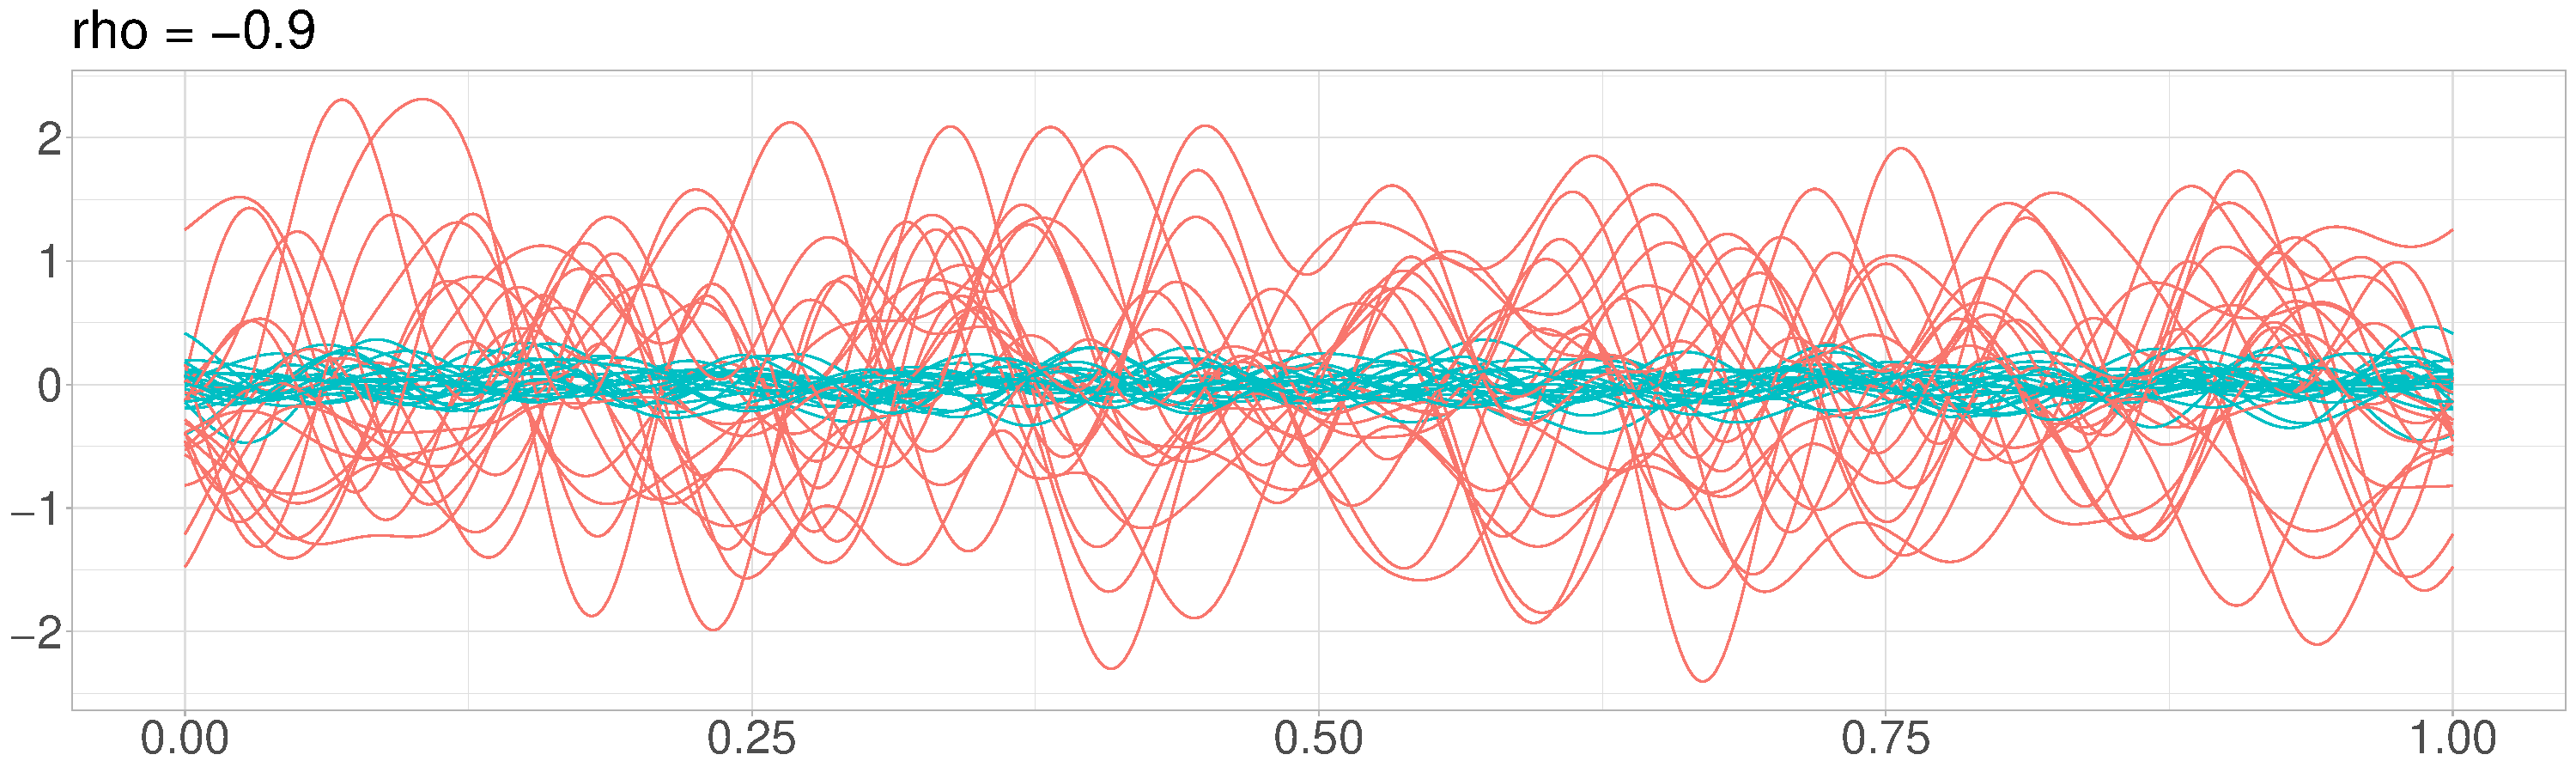
\includegraphics[width=1.1\textwidth]{../Graphics/rho0_9_comparison.PDF}
				}
				\caption{Artifact of the Curve Fitting Procedure \\
				sample 1 in red, sample 2 in blue}
				\label{curve_fitting_artefacts}
			\end{figure}
			These processes are constructed as described in Section \ref{Simulation_Study} for a choice of $\rho_2(t) = -0.9$. This implies that the data generating process generates data with a point-wise variance of one. However, due to the structure of the data, the curve fitting procedure fails to conserve this property. Therefore, artifacts, such as the one shown in Figure \ref{curve_fitting_artefacts}, can heavily influence the power of the constructed test, meaning that it could be advisable to change the approach to one of the following.
			\begin{enumerate}
				\item \textbf{Comparisons at the discrete data points.} Suppose observations are discrete but dense enough to be interpreted as smooth curves. In that case, one could use the points where data is observed to compare the functions generated for the approximation of the CvM test to the original samples. This approach is close to the one described in \cite{bugni_permutation_2021} for the case of discrete observations.
				\item \textbf{Linear Interpolation.} Instead, one could use linear interpolation of the original curves to compare them to the generated curves. This would preserve the functional nature while not generating the fitting artifacts shown in Figure \ref{curve_fitting_artefacts}.
			\end{enumerate}
			The simulations in Sections \ref{Simulation_Study} use the first approach, as it limits the computational cost of the procedure while staying close to the original paper. The same problem occurs for the mean-focused test. In this case, linear interpolation between the discrete points is used to approximate the mean function on the full interval.

		
	\section{Test for Persistence Alternatives}\label{variant}
		One particular application for the CvM type test presented in \cite{bugni_permutation_2021} is a slight modification leading to a test for differences in the persistence structure of the data generating processes. This test is an interesting extension as there are few existing methods that test a similar null hypothesis.\\
		
		To give some context: in the literature, there are already many methods to test whether two samples share a common mean function. 
		\cite{cox_pointwise_2008} propose a method that compares functions point-wise using a multiple comparison procedure introduced by \cite{westfall_resampling-based_1993}. They show that this approach can be used to approximate a continuum of comparisons as the grid used to compare points gets finer.
		\cite{lee_two_2015} introduce a method based on the adaptive Neyman methodology and a functional principal component approach to test whether two samples share a common mean function.
		\cite{fan_test_1998} also develop a method based on adaptive Neyman methodology to compare multiple samples. However, their procedure uses wavelet thresholding techniques developed in the authors' earlier works. 
		
		There is also a considerable number of tests for differences in the covariance functions of processes, such as the tests presented in the following papers. 
		\cite{guo_testing_2018} develop a method based on the supremum of the integrated squared difference between the sample covariance functions of the individual samples and the pooled sample. Test decisions are then made using critical values derived via bootstrapping approaches.		Building on their previous work, \cite{guo_new_2019} propose an additional test that generalizes the idea of the point-wise F-test as described, for example, in \cite{ramsay_functional_2005}. In their approach, the authors extend existing ideas such as the $F_{\textit{max}}$-test or the quasi-GPF trying to answer the corresponding global hypothesis to compare the covariance functions of multiple functional populations.

		However, there are few tests that specifically address differences in the persistence of processes including higher cross-moment functions and the proposed procedure adds to the limited arsenal.\\
		
		\subsection{Null-Hypothesis}
		Let $\{X_i(t) \ | \  i = 1, \dots, n\}$ and $\{Y_i(t) \ | \  i = 1, \dots, m\}$ again denote the samples under consideration. Assume that the samples consist of i.i.d. realizations of random functions $X(t)$ and $Y(t)$.
		To focus on the persistence properties of the random functions, define the standardized counterparts to these random functions in the following way.
		\begin{multicols}{2}
			\noindent
			\begin{equation*}
				\begin{split}
					\mu_{X}(t) = &\mathbb{E}\left[X(t)\right] \\
					\sigma_{X}(t) = &\sqrt{\mathbb{E}\left[X(t) - \mu_{X}(t)\right]^2}
				\end{split}
			\end{equation*}
			\begin{equation}
				\begin{split}
					\mu_{Y}(t) = &\mathbb{E}\left[Y(t)\right] \\
					\sigma_{Y}(t) = &\sqrt{\mathbb{E}\left[Y(t) - \mu_{Y}(t)\right]^2}
				\end{split}
			\end{equation}
		\end{multicols}
		Then the standardized random variables can be defined as follows.
		\begin{multicols}{2}
			\noindent
			\begin{equation*}
				\tilde{X}(t) = \frac{X(t) - \mu_{X}(t)}{\sigma_{X}(t)}
			\end{equation*}
			\begin{equation}
				\tilde{Y}(t) = \frac{Y(t) - \mu_{Y}(t)}{\sigma_{Y}(t)}
			\end{equation}
		\end{multicols}
		Their distribution functions can be defined analogously to Section \ref{Bugni_Horowitz_2021} and shall be denoted by $F_{\tilde{X}}(z)$ and $F_{\tilde{Y}}(z)$ respectively in the following. Then a modified null hypothesis similar to \cite{bugni_permutation_2021} can be formulated with respect to the distribution functions of the standardized random variables.
		\begin{equation}
			\begin{split}
				H_0: \quad &F_{\tilde{X}}(z) = F_{\tilde{Y}}(z) \quad \forall z \in \mathbb{L}_2[0.1] \\
				H_1: \quad &\mathbb{P}_{\mu}\left[F_{\tilde{X}}(z) \neq F_{\tilde{Y}}(z)\right] > 0
			\end{split}
		\end{equation}
		As the standardization eliminates all differences in these processes' mean and variance patterns, one of the distinct remaining features that might differentiate these processes are their persistence properties.
		Somewhat more technical, this hypothesis is linked to the equality of the cross-moment functions of the underlying processes after standardization.
		Therefore, this focused approach could be tailored by choosing an appropriate $\mu$ to detect differences in this general idea of persistence of the data generating processes. \\
		
		\subsection{Test-Procedure}\label{persistence_test}
		The modified test is functionally nearly identical to the CvM type test described in \cite{bugni_permutation_2021}. However, it adds a standardization step in the calculation of the test statistic to eliminate differences in the mean functions of the processes and their variance structure. In each permutation step, the calculation of the test statistic is thus described by the following algorithm.\\
		
		\noindent\fbox{%
			\parbox{\textwidth}{%
				\vspace{0.1cm}
		Let $\mathcal{W} = \{W_i(t) \ | \ i = 1, \dots, n\}$ be sample one and $\mathcal{V} = \{V_i(t) \ | \  i = 1, \dots, m\}$ be sample two. These samples are generated by randomly permuting the original samples $\{X_i(t) \ | \  i = 1, \dots, n\}$ and $\{Y_i(t) \ | \  i = 1, \dots, m\}$.
		\begin{enumerate}
			\item Calculate the sample mean functions for the permuted samples: \\
			$\bar{W}(t) = \frac{1}{n} \sum_{i = 1}^{n} W_i(t)$ and $\bar{V}(t) = \frac{1}{m} \sum_{i = 1}^{m} V_i(t)$
			\item Center the sample curves to obtain centered permutation samples: \\
			$\bar{\mathcal{W}} = \{W_i(t) - \bar{W}(t) \ | \ i = 1, \dots, n\}$ and $\bar{\mathcal{V}} = \{V_i(t) - \bar{V}(t) \ | \ i = 1, \dots, m\}$
			\item Calculate the point-wise standard deviations: \\
			$\sigma_{\mathcal{W}}(t) = \sqrt{\frac{1}{n}\sum_{i = 1}^{n}\left[W_i(t) - \bar{W}(t)\right]^2}$ and $\sigma_{\mathcal{V}}(t) = \sqrt{\frac{1}{m}\sum_{i = 1}^{m}\left[V_i(t) - \bar{V}(t)\right]^2}$
			\item Standardize the observations in the permuted samples:\\
			$\tilde{\mathcal{W}} = \{\frac{W_i(t) - \bar{W}(t)}{\sigma_{\mathcal{W}}(t)} \ | \ i = 1, \dots, n\}$ and $\tilde{\mathcal{V}} = \{ \frac{V_i(t) - \bar{V}(t)}{\sigma_{\mathcal{V}}(t)} \ | \ i = 1, \dots, m\}$
			\item Calculate $\hat{\tau}_{n,m}$ for the standardized permutation samples $\tilde{\mathcal{W}}$ and $\tilde{\mathcal{V}}$ as described in Section \ref{Bugni_Horowitz_2021} for a chosen measure $\mu$.
		\end{enumerate}
			}
		}\vspace{0.3cm}
		The overarching test procedure is again given by the derivation of a permutation distribution and a permutation test decision according to the rules stated in Section \ref{Permutation_Tests}.\\
		
		Due to the introduction of the standardization step, the problem described in Section \ref{problem_curve_fitting} is potentially of even greater importance than in the previous section. As the test relies on standardizing the objects used for the calculation of the test statistic, it would be of immense importance whether curve fitting is employed and at what step of the procedure it is introduced. For example, if standardization would be applied to discrete observations, which are then fitted using a functional basis, the resulting curves would generally not be standardized in the desired way. This can be seen in Figures \ref{persistence_samples} and \ref{persistence_samples_basis_problem} in Appendix \ref{add_figures} which show samples that were generated by processes with a point-wise mean of 0 and a point-wise variance of 1 and their fitted counterparts. 
		Using curve-fitting in this way could create simulations indicating a strong power against persistence alternatives. However, this power might entirely be based on the artifacts created by the curve fitting procedure.\\
		Therefore, it is advisable to either perform standardization on the fitted curves if curve fitting is desired because of the data itself, or to rely on comparisons between the discrete observations and the curves created for the approximation of the CvM type test statistic. For the purposes of this thesis the latter approach will be used. This can be seen as analogous to the variant of the CvM type test for discrete data described in \cite{bugni_permutation_2021}.
		
	\section{Simulation Study}\label{Simulation_Study}
		To learn more about the potential practical applications of this method, it is helpful to study its properties in a series of simulations. \cite{bugni_permutation_2021} studied an array of different setups that give an idea of the performance in a collection of settings, and this thesis will replicate some of these results and explore some where the method struggles.
		
		The simulations presented as part of this thesis have been conducted on \textit{bonna}\footnote{\href{https://www.dice.uni-bonn.de/de/hpc/hpc-a-bonn/infrastruktur}{https://www.dice.uni-bonn.de/de/hpc/hpc-a-bonn/infrastruktur}}. \textit{bonna} is the high performance computing cluster provided by the University of Bonn. However, slight modifications of the provided code suffice to run it on personal computers.\\

		All analyses in this thesis have been conducted with R\footcite{R}. As a supplement to this thesis, the two-sample variant of the test taken from \cite{bugni_permutation_2021} is implemented in an R package called \textit{PermFDATest}. The R package and all code that has been used to produce the following results is publicly available as part of a GitHub repository\footnote{\href{https://github.com/JakobJuergens/Masters_Thesis}{https://github.com/JakobJuergens/Masters\_Thesis}} that complements this thesis.
		The package makes extensive use of the implementations by \cite{fda} and \cite{tidyverse}.

		\subsection{Simulation Setup}
		The simulations presented in this thesis, are inspired by the simulation study from \cite{bugni_permutation_2021} and shine more light on specific settings that offer insight into the potential benefits and problems of the method. 
		To describe the specific processes used in the simulation, this Section introduces the notation used in \cite{bugni_permutation_2021} shortly to then describe the data generating processes mathematically. \\
		
		Deviating from \cite{bugni_permutation_2021}, these simulations focus on the two-sample variant of the test. Additionally, the data are generated on the closed interval $\left[0,1\right]$ and use a smaller sample size of $20$ observations per sample. Therefore, let $\mathcal{T} = \left\{0, 0.01, 0.02, \dots, 1\right\}$ be the index set of the discrete points on the unit interval, then the observations are constructed in the following way.\\
		
		\noindent\fbox{%
			\parbox{\textwidth}{%
		\begin{enumerate}
			\item Draw random variables $\left\{\xi_{i,s} \ \vert \ (i,t) \in \left\{1, \dots, 20\right\} \times \mathcal{T} ; s = 1,2 \right\}$ independently from the $\mathcal{N}(0,1)$ distribution.
			\item For all $i = 1, \dots, 20$ and $s = 1,2$, set $\tilde{X}_{i,s}(0) = \xi_{i,s}(0)$.
			\item For all $i = 1, \dots, 20$; $s = 1,2$ and $t = 0.01, \dots, 1$, set $\tilde{X}_{i,s}(t) = \rho_{s}(t)\tilde{X}_{i,s}(t-0.01) + \xi_{i,s}(t)\sqrt{1-\rho_s^2(t)}$ where $\rho_{s}(t)$ is a parameter as defined below.
			\item For all $i = 1, \dots, 20$; $s = 1,2$ and $t \in \mathcal{T}$, set $X_{i,s}(t) = \mu_s(t) + \sigma_s(t)\tilde{X}_{i,s}(t)$ where $\mu_s(t)$ and $\sigma_s(t)$ are parameters as defined below.
		\end{enumerate}
		The resulting random variables $\left\{X_{i,s}(t) \ \vert \ t \in \mathcal{T}; \ i = 1, \dots, 20; \ s = 1,2\right\}$ are normally distributed with the following properties.
		\begin{multicols}{2}
			\begin{enumerate}
				\item $\mathbb{E}\left[X_s(t)\right] = \mu_s(t)$
				\item $\text{Var}\left[X_s(t)\right] = \sigma^2_s(t)$
				\item $\text{Corr}\left[X_s(t), X_s(t-0.01)\right] = \rho_s(t) \\ \forall t \in \mathcal{T} \ \text{with} \ t > 0.01$
			\end{enumerate}
		\end{multicols}
			}
		}
		\vspace{0.2cm}
		
		This thesis focuses on three distinct violations of the null hypothesis described in the following. For each of the following settings sample 1 is generated from the same process as a reference point to compare the different settings. Therefore, the parameters for sample 1 are therefore chosen as follows.
		\begin{multicols}{2}
			\begin{enumerate}
				\item $\mu_1(t) = 0 \quad \forall t = 0.01, \dots, 1$
				\item $\sigma_1(t) = 1 \quad \forall t = 0.01, \dots, 1$
				\item $ \rho_1(t) = 0.5 \quad \forall t = 0.01, \dots, 1$
			\end{enumerate}
		\end{multicols}
		
		For the second sample, three different violations of the null hypothesis and a benchmark case where the null hypothesis is correct are generated.
		\begin{enumerate}
			\item \textbf{Identical Data Generating Processes}\\
				  The first setting is the benchmark where both samples are generated using the same random function. This setting is meant to support the theoretical points arguing that the permutation tests described in this thesis have the correct size.
			\item \textbf{Mean Shift}\\
				  The second setting introduces a shifted mean function. This is one possible violation where \cite{bugni_permutation_2021} describe weak power of the Cramer-von Mises type test. Deviating from sample 1, sample 2 has mean function 
				  $$\mu_2(t) = x (x-1) \quad t \in \mathcal{T}$$
			\item \textbf{Correlation Shift}\\
			 	  The third setting violates the null hypothesis by changing the correlation structure between neighboring observations. Here, observations are less persistent due to a lower, but still constant choice of the correlation parameter.
			 	  $$\rho_2(t) = 0 \quad \forall t = 0.01, \dots, 1$$
%			 	  This setting can therefore be seen as testing for alternatives consisting of variations of the persistence structure of a random function.
			\item \textbf{Variance Shift}\\
				  In the fourth simulation setting, the point-wise variance function is altered in the following way.
				  $$\sigma_2(t) = 1 + 0.5t \quad \quad t \in \mathcal{T}$$
		\end{enumerate}
	
		Figure \ref{settings} shows samples generated by these processes. As can be seen there, the difference between the samples is optically quite subdued. Therefore, a high power against these alternatives is not expected. However, any nontrivial power shown in these settings is a good indicator for the qualities of the test.
		\begin{figure}[H]
			\makebox[\textwidth][c]{
				\includegraphics[width = 1.1\textwidth]{../Graphics/Settings\_comparison.PDF}
			}
			\caption{Samples generated for the four settings. \\
			Sample 1 in red, Sample 2 in blue}
			\label{settings}
		\end{figure}
		
		But before performing the simulations, there is a number of parameter choices that has to be made to as explained in the theoretical description of the test.
		
		\noindent\fbox{%
			\parbox{\textwidth}{%
		\begin{enumerate}
			\item As shown in the mathematical construction of the data, these simulations compare samples consisting of a smaller number of observations per sample $n=20$ and focus on the two-sample version of the test. Additionally, each observation is constructed from a lower number of discrete observations (101) than in the original paper.
			\item Concerning the choice of the truncation parameter $K$, which is used in the construction of the measure $\mu$ as shown in Equation \ref{truncation}, the authors argue that their simulations showed that the power of the test became flat at about $K = 20$ and chose $K = 25$. For the sake of reproducing their results, the same parameter was used in this thesis.
			\item Another parameter that has to be chosen is $L$, determining the number of functions used in the approximation of the test statistic $\hat{\tau}_{n,m}$ by Monte-Carlo integration as shown in Equation \ref{tau_hat}. \cite{bugni_permutation_2021} chose $L = 4000$ and preliminary testing confirmed that this choice seems reasonable in many settings when combined with reasonable choices for the construction of the measure $\mu$. However, problems such as the one described in Section \ref{problem_curve_fitting} might be closely connected to this choice.
			\item For the number of permutations $Q$ used for the approximation of the permutation distribution of both test statistics the authors chose a value of $Q = 500$. This thesis uses the same parameter. However, absent strong computational limitations a higher choice for $Q$ could benefit the properties of the tests.
			\item For the construction of the measure $\mu$, the weight function $w(t)$ has to be chosen. In this simulation, the weight function is chosen as in the empirical application in \cite{bugni_permutation_2021}. This approach is described in Section \ref{mu} as the first approach listed for the choice of $w(t)$. 
			\item Deviating from the original authors' choice due to preliminary tests, the sequence $\left(\rho_i\right)_{i = 1, \dots, K}$ is determined by checking the sample standard deviation of the corresponding Fourier coefficients in the first sample obtained by fitting the same basis that is used in the construction of $\mu$ to the observations. These are then multiplied by a constant factor to increase variability in the functions drawn from $\mu$. This higher variability seemed to improve performance in preliminary tests, but should be studied in further experiments.
			\item Using the same choice as in the original paper, the simulations use independent standard normal error terms $U_k \quad k=1, \dots, K$ for the Fourier coefficients shown in Equation \ref{Fourier_coefs} for the construction of the measure. As the processes under consideration are Gaussian by construction and thereby have thin tails, this choice should be reasonable following the authors' argumentation.
		\end{enumerate}
			}
		}
		
		\subsection{Results}
		Taking a look at the results from the simulation study, it is interesting to compare the empirical rejection probabilities for different types of violations of the null hypothesis.
		
		\begin{table}[H]
			\centering
			\begin{tabular}{l|c|cccc}\toprule
				\textbf{Test}	&$\left(\alpha_{\tau}, \alpha_{\nu}\right) $ &\textbf{Setting 1} &\textbf{Setting 2}	&\textbf{Setting 3} &\textbf{Setting 4}\\
				\midrule
				Means-Test		&$\alpha_{\nu} = 0.05$	& 0.058		& 0.5  	 	& 0.04709	& 0.058 	\\
				CvM-Test 		&$\alpha_{\tau} = 0.05$	& 0.03775	& 0.55675  	& 0.63978 	& 0.9585	\\
				\midrule	
				Combined		& (0.04, 0.01)			& 0.04		& 0.577  	& 0.5977 	& 0.9535	\\
								& (0.03, 0.02)			& 0.043		& 0.587  	& 0.5516 	& 0.942 	\\
								& (0.025, 0.025)		& 0.045		& 0.576  	& 0.53148 	& 0.938		\\
								& (0.02, 0.03)			& 0.044		& 0.564  	& 0.51102 	& 0.932		\\
								& (0.01, 0.04)			& 0.046		& 0.558  	& 0.42929 	& 0.896		\\
				\bottomrule
			\end{tabular}
			\caption{Empirical Rejection Probabilities}
		\end{table}
		Looking first at setting 1, which is a simulation under the null hypothesis, the rejection probabilities seem to be compatible with the chosen size of $0.05$. However, the size of the rejection frequency for the CvM test seems slightly low, which could be an artifact caused by the relatively low number of simulation runs. A larger simulation using $10000$ runs for the CvM type test resulted in a rejection frequency of 0.0469 and therefore seems to confirm this hypothesis.
		Next, looking at the rejection frequencies of the mean-based test in settings 3 and 4, the test shows only trivial power. This is expected as the samples were explicitly generated by processes sharing a common mean function. 
		
		For setting 2, which is a mean shift between the processes the power of both tests is relatively high considering the low sample size of $20$. Especially considering the fact that the authors mentioned that the power of the CvM type test in pure mean shift settings is somewhat lacking. However, this can be remedied by the fact, that even thought the mean shift is rather subdued visually, it is stronger than the mean shift used in the simulation study of \cite{bugni_permutation_2021}.
		
		Due to the change in setting 3, picking up the differences in the persistence structure might be difficult with a measure induced by a random variable that was truncated at a low truncation parameter $K$. However, for a choice of $K = 25$, the simulation shows considerable non-trivial power against this alternative. The fact that the combined tests keep a lot of their power as the level of the CvM test decreases while the mean-focused test shows no non-trivial power, indicates that even at higher significance levels, a comparatively high fraction of violations of the null hypothesis can be identified by the CvM test.
		
		In setting 4, the rejection frequencies are extremely high, which in light of the other three settings and the visual presentation of exemplary samples in Figure \ref{settings} is unsurprising. In the Figure, setting 4 showed the clearest difference between the reference sample and sample 2 and the test was able to pick up on it. Similar to setting 3, the rejection frequencies for the combined tests indicate that the rejection frequency of the CvM type test remained high even at stricter significance levels.
	
		\subsection{Simulation - Test for Persistence Alternatives}\label{sim_persistence}
		Using simulations akin to setting 3, it is possible to test the proposed test for persistence alternatives from Section \ref{variant}. However, due to computational constraints, this simulation currently cannot follow the real test's structure and shall instead serve as a heuristic for the real test's performance. \\
		Primarily, the simulation differs from the proposed test in the following way to reduce computational cost while staying reasonably accurate in the proposed simulation setting. The standardization step makes it necessary to perform the comparison between functions that is performed in the calculation of the CvM test statistic in each permutation step. This massively increases the computational cost. Therefore, as a heuristic for the real test, these simulations are performed without a standardization step. However, a data generating process with a mean function $\mu(t) = 0$ and a point-wise variance function $\sigma(t) = 1$ is used. Therefore, in expectation, sample equivalents will share these characteristics. However, individual samples may not. \\
		Due to this concession to limited computational resources, the following simulation results could potentially overstate the power of the test against alternatives as described above. This is caused by potential differences in the sample mean and point-wise sample variance present in the permuted samples that would have been removed by standardization. 
		However, in the proposed test structure the possibility to specifically test for alternatives in the persistence structure is a significant advantage.\\
	
		The results for different correlation parameters are given in the following tables. Again, the same reference process with $\rho_1(t) = 0.5$ generated the reference sample.
%		\begin{table}[H]
%			\centering
%			\begin{tabular}{lccccc}\toprule
%				$\alpha_{\tau}$ &$\rho_2(t) = -0.9$ &$\rho_2(t) = -0.5$ &$\rho_2(t) = 0$ &$\rho_2(t) = 0.5$ &$\rho_2(t) = 0.9$\\
%				\midrule
%				$0.05$	& 0.830 & -  &  0.250	& 0.0415   & - \\
%				$0.01$ 	& 0.783	& -  &  0.119	& 0.0104   & -  \\
%				$0.001$	& 0.735	& -  &  0.0492	& 0.00261  & -  \\
%				\bottomrule
%			\end{tabular}
%			\caption{Empirical Rejection Probabilities}
%		\end{table}
%	                                          	
%		The apparent power of this test comes in part from the basis that is used to fit the data. Even though standardization of the original observations as described in approach one shown in Section \ref{persistence_test} ensures that the discrete data itself has a point-wise sample variance of one, the method that is used to fit the observations can lead to curves that are highly dissimilar between samples once the data points are fitted. 
%		Figure \ref{curve_fitting_artefact} shows a rather extreme case for the case of $\rho_1(t) = 0.5$ and $\rho_2(t) = -0.9$. In Appendix \ref{add_figures} Figure \ref{persistence_samples} shows some original data sets generated for these simulations.These are contrasted by Figure \ref{persistence_samples_basis_problem} which shows the same samples fitted using a Fourier basis containing 25 functions. 
%		Even though the underlying data generating processes have an identical point-wise variance, the method that is used to fit the discrete observations, creates potentially distorting artifacts.
%
%		Variant one can be seen as close to approach two from Section \ref{persistence_test} as the standardization is applied to every point that is actually considered during the comparison of the functions for the Cra\'{e}r-von Mises test. The point-wise functional standardization mentioned in \ref{persistence_test} is computationally intensive and requires a more advanced method of comparison between functions. 
%		However, as variant one described above can be seen as a heuristic for its performance, I performed a second simulation using this approach, leading to the results presented in Table \ref{rej_probs_cor}. These could potentially be a better approximation of the power of the test procedure as the rejections do not rely on artifacts created by the process of fitting a functional basis to the discrete observations.
		\begin{table}[H]
			\centering
			\begin{tabular}{l|ccccc}\toprule
				$\alpha_{\tau}$ &$\rho_2(t) = -0.9$ &$\rho_2(t) = -0.5$ &$\rho_2(t) = 0$ &$\rho_2(t) = 0.5$ &$\rho_2(t) = 0.9$\\
				\midrule
				$0.05$	& 0.198 & 0.858  &  0.640 & 0.048   & 0.977  \\
				$0.01$ 	& 0.044	& 0.623  &  0.393 & 0.009   & 0.913  \\
				$0.001$	& 0.016	& 0.385  &  0.197 & 0.002   & 0.734  \\
				\bottomrule
			\end{tabular}
			\caption{Empirical Rejection Probabilities}
			\label{rej_probs_cor}
		\end{table}
		These results show multiple things. First, as expected the size of the test, approximated by the case $\rho_2(t) = 0.5$ is close to the chosen nominal level. Due to the properties of permutation tests, this is not a surprise as it holds by construction. Second, the other cases, which approximate power against specific alternatives, are interesting as they are in part counter-intuitive.
		
		In most settings, one would typically assume that the rejection frequency increases as the parameter that specifies the deviation from the null hypothesis changes away from its equivalent in the reference sample. These simulations, however, show that for the case of $\rho_2(t) = -0.9$ the opposite happens. Even though the persistence parameter is even further away from $0.5$ than for the case of $\rho_2(t) = -0.5$, the rejection frequency decreases. This could be linked to the measure that is used for the calculation of the test statistic. As the parameter decreases, the curves are less persistent, meaning that Fourier functions of higher frequency would be needed to approximate them. However, if due to the truncation, it is not possible to use appropriately high-frequent functions in the CvM test, the performance might suffer. This is just a first hypothesis that could be studied in more detail using further simulations with different persistence parameters and different truncation parameters for the basis used to construct the measure.\\
		
		{\color{red} Hier weiterschreiben.}
				
	\section{Application}\label{Application}
		In order to give an example for the real-world merits of the method, this section will compare electricity demand data from Adelaide. This data is provided as part of the \textit{fds}\footcite{fds} package for R. It presents half-hourly energy demand in megawatts and was originally used by \cite{magnano_generation_2007} and \cite{magnano_generation_2008}. It contains electricity demand curves for 3556 days from 6/7/1997 to 31/3/2007. Some of these curves, specifically a selection of curves observed on Wednesdays and Saturdays fitted using a Fourier basis consisting of 25 functions, is shown in Figure \ref{electricity_demand}.
		\begin{figure}[H]
			\makebox[\textwidth][c]{
				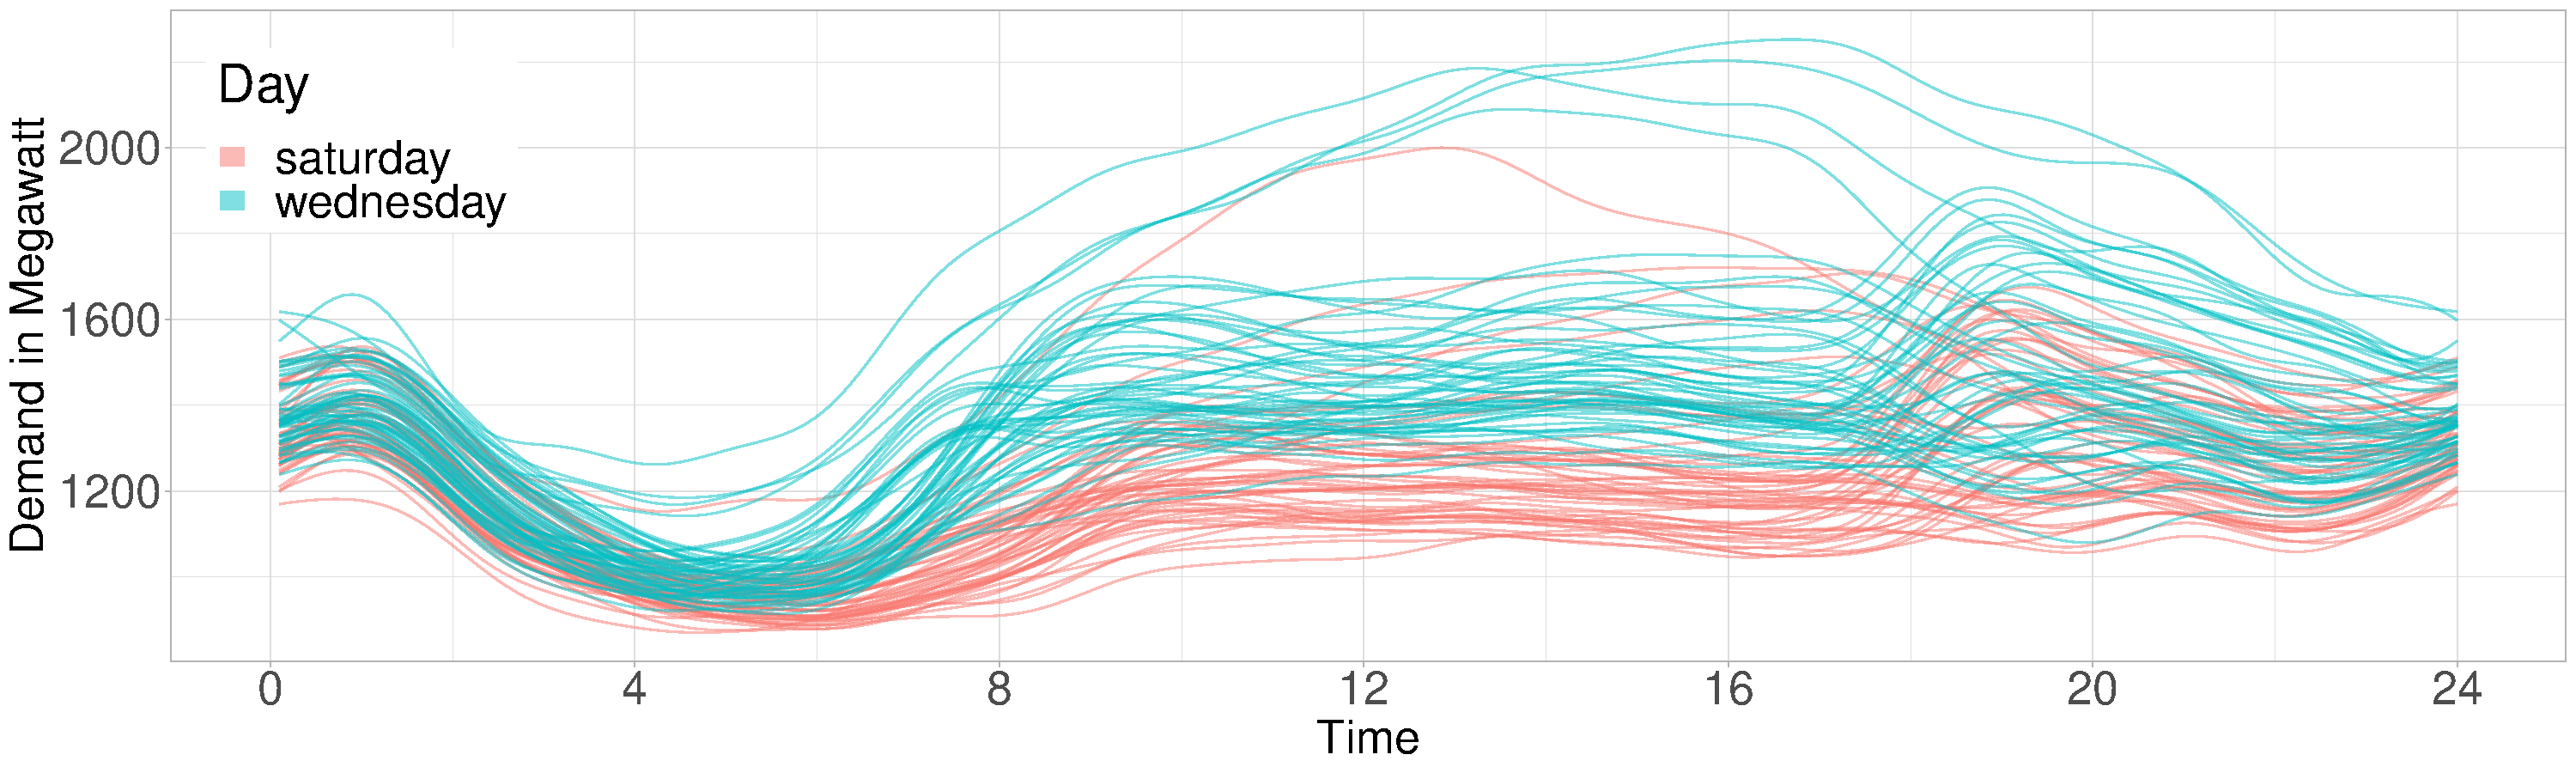
\includegraphics[width=1.1\textwidth]{../Graphics/electricity_demand_curves.PDF}
			}
			\caption{Electricity Demand in Adelaide}
			\label{electricity_demand}
		\end{figure}
	
		The specific question studied with the method presented in this thesis is whether electricity demand on working days and weekends can be seen as if they were generated by the same stochastic process. However, due to information obtained during the data cleaning step, that indicates a violation of the i.i.d. assumption, the observations for the weekend will be limited to Saturdays. 		
	
		\subsection{Data Cleaning and Preprocessing}
		Before actually applying the test from \cite{bugni_permutation_2021}, it is important to prepare the data for the procedure. As this problem does not have the structure that an experiment as described in \cite{bugni_permutation_2021} possesses, some problems have to be addressed before using the procedure. These adjustments are described below and some details are substantiated in Appendix \ref{Application_Appendix}.
		
			\subsubsection{Removal of Mondays and Fridays}
			One potential problem of this procedure is the question whether observations on different weekdays or days of the weekend can be seen as independent and identically distributed. While it seems reasonable to assume that demand may be similar on Saturdays and Sundays, it is questionable whether the same can be said for working days. 
			One potential problem is the ramping up and down of industrial production and commercial activity on Mondays and Fridays. Therefore, I decided to exclude these days from my analysis and only compare the weekend with Tuesdays, Wednesdays and Thursdays.
			
			\subsubsection{Holidays}
			Furthermore, holidays could appear more regularly on specific weekdays than others. Whereas on weekends, a holiday would not significantly influence the electricity demand due to the already reduced economic activity, this is different for weekdays. Therefore if holidays would occur systematically more often on specific days - such as for example Thursdays for the case of Germany - this could create problems. Therefore public holidays in Southern Australia, the Australian federal territory containing Adelaide, were excluded in the analysis. A list of holidays that were excluded is given in Appendix \ref{Application_Appendix}. Additionally, days immediately before and after holidays are excluded due to the same reason as Mondays and Fridays. This procedure of eliminating holidays from the data set removed 299 out of 3556 curves from the data set which was used in further steps of the analysis. 
			
			\subsubsection{Curve Fitting}
			To employ methods that are suitable to remove trend and seasonal components from the data, it is useful to fit a functional basis to the underlying discrete observations. However, as described in Section \ref{problem_curve_fitting}, this can lead to problems, if the truncated functional basis is unable to capture the features of the discrete data. However, in the setting explored in this application, visual inspection of the resulting curves showed no signs of artifacts created by the curve fitting process. This makes sense from a theoretical perspective, as the curves are more persistent than those explored in the simulations. Therefore, the truncated basis, consisting of trigonometric functions of lower frequencies, should be able to capture the curves' properties appropriately.
			
			This, in turn, makes the removal of trend and seasonal components from the fitted curves more attractive, as it more closely addresses the functional nature of the underlying data generating processes. Therefore, for the purposes of this simulation, a Fourier basis consisting of 25 functions was fitted to the original data to perform the data cleaning step.
			
			\subsubsection{Detrending and Deseasoning}
			A third potential problem of this data set is its functional time series structure. For example, electricity demand might be systematically higher in the summer months due to the added energy consumption of air-conditioning units. Therefore, a simple interpretation of the data as generated by an i.i.d. process might be unsubstantiated and additional steps have to be made before the procedure can be justified. \\
			Additionally, it might be the case that electricity demand has a trend component that has to be removed before this method can reasonably be applied to this data. To combat this low frequency seasonal component due to the seasons and a potential long-term trend I specify a model as follows and demean the data as described below. For the estimation of this model, holidays and days immediately before and after holidays are excluded. Mondays and Fridays are included and removed from the data set after the estimation for the creation of the samples that are used to apply the method described in this thesis.
			\begin{equation}\label{Data_Cleaning}
				\begin{split}
					f_{\textit{demand}} = &f_{\textit{mean}} + f_{\textit{trend}}(\textit{year} - 1997) + \sum_{j = 2}^{12}\mathbbm{1}_{\left[\textit{month}\: = \: j\right]}f_{\textit{month}, j}\\
					 &+ \sum_{k = 2}^{7}\mathbbm{1}_{\left[\textit{day}\: = \: k\right]}f_{\textit{day}, k} + f_{\textit{random}}
				\end{split}	
			\end{equation}
			This is estimated with the usual theory for function-on-scalar regression which is described for example in \cite{ramsay_functional_2005}. Then, the following objects are used for the further treatment.
			\begin{equation}
				\tilde{f} = f_{\textit{mean}} + \sum_{k = 2}^{7}\mathbbm{1}_{\left[\textit{day}\: = \: k\right]}\hat{f}_{\textit{day}, k} + \hat{f}_{\textit{random}}
			\end{equation}
			The function-on-scalar regression described in Equation \ref{Data_Cleaning} was performed in R using the \textit{fda}\footcite{fda} package and gave the following results. As these are the results of a function-on-scalar regression, it is convenient to plot the resulting estimates as they are functions instead of giving the estimated Fourier coefficients.
			The estimated coefficient functions for the different weekdays are of special interest as they are directly linked to the problem that is to be studied using the method from \cite{bugni_permutation_2021}. In this case Sunday is the baseline and these curves describe the deviation relative to it.
			\begin{figure}[H]
				\makebox[\textwidth][c]{
				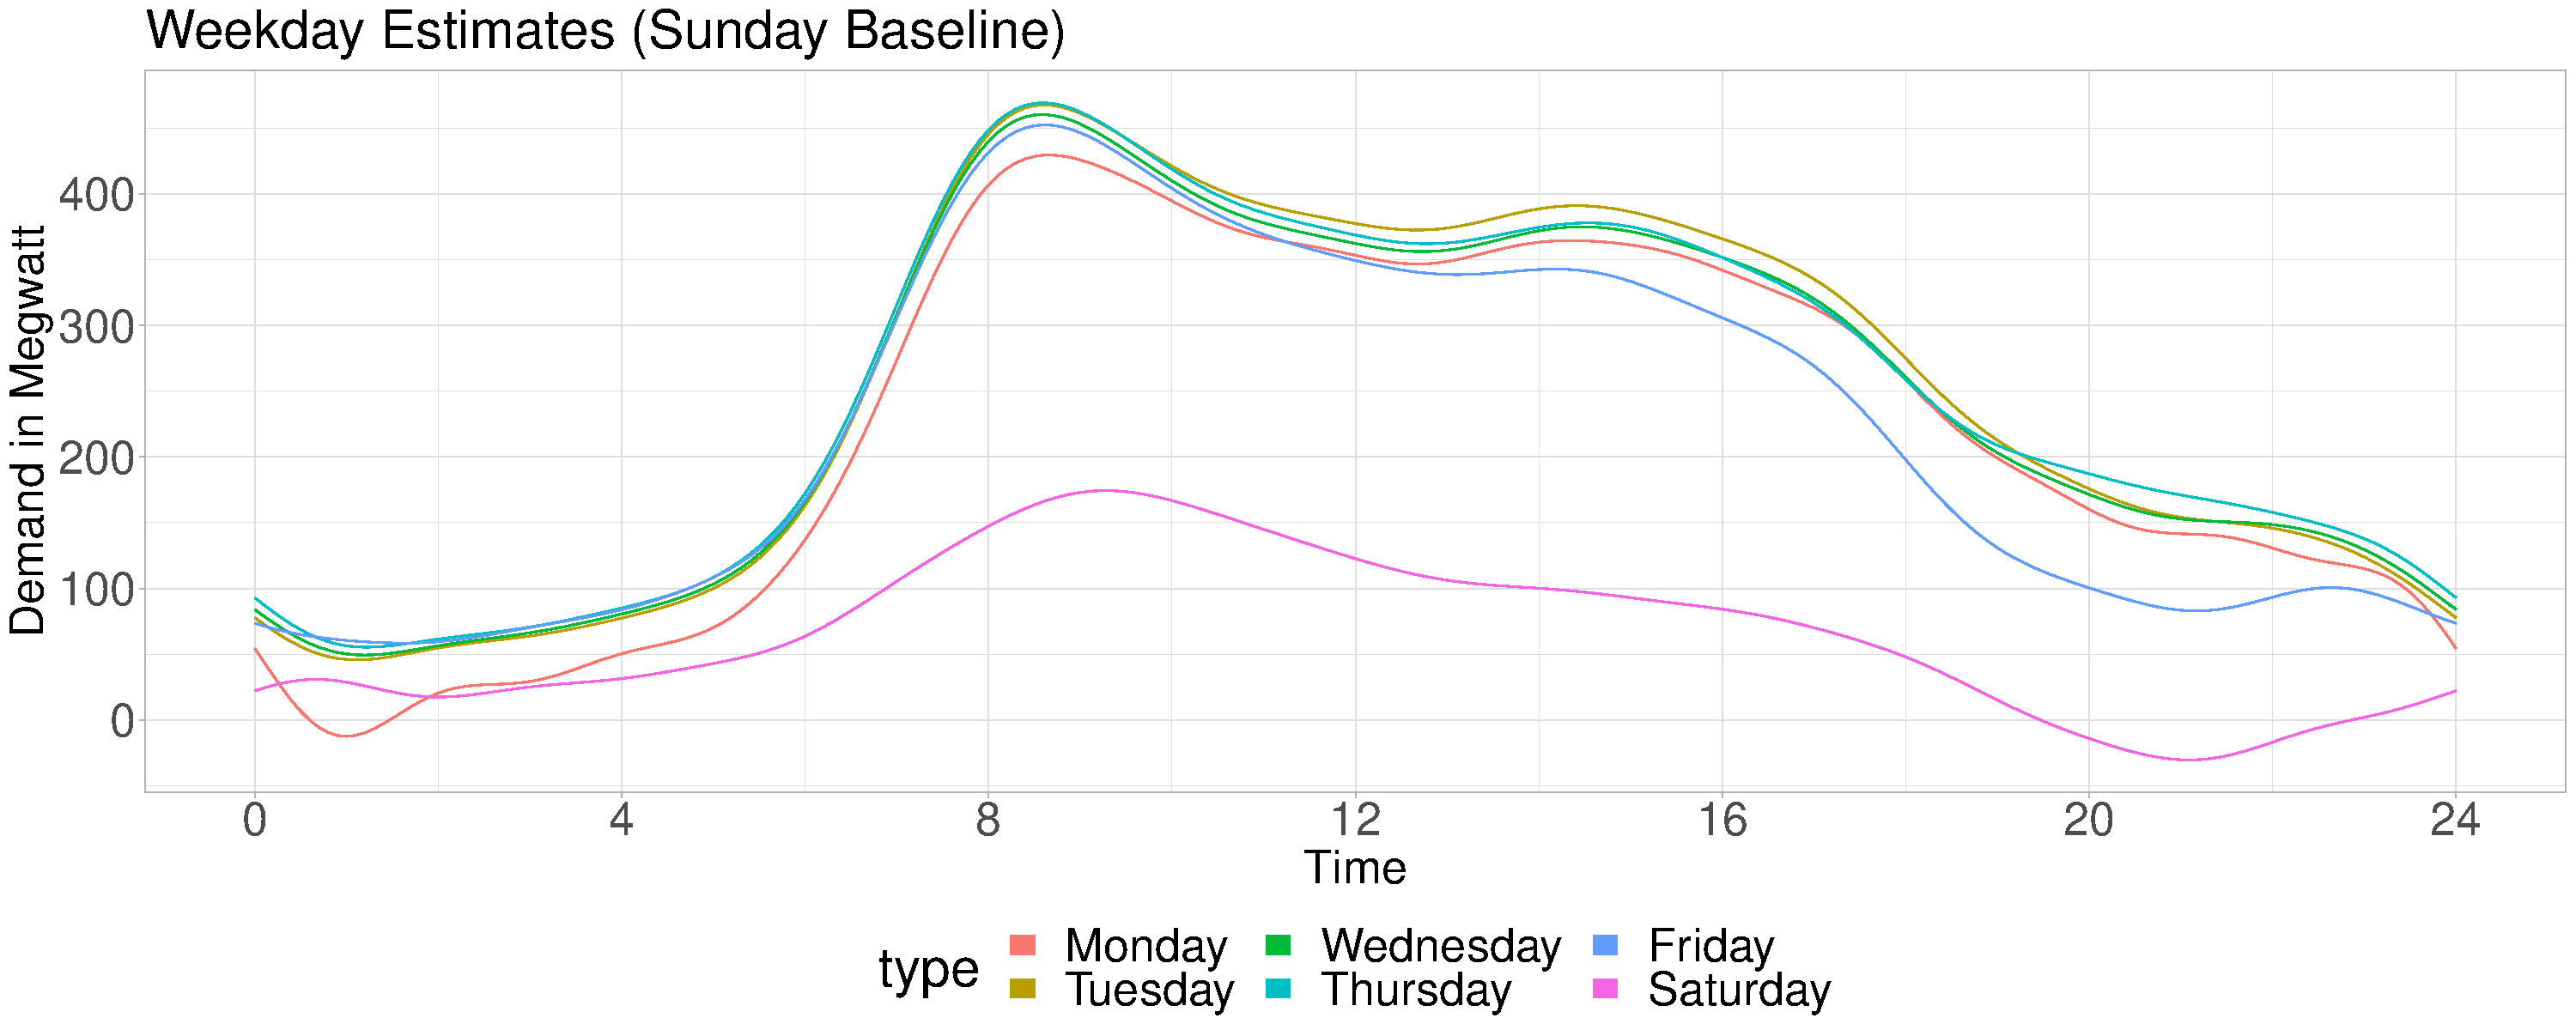
\includegraphics[width=1.1\textwidth]{../Graphics/estimate_weekdays.PDF}
			}
				\caption{Estimates for the weekdays (Sunday as baseline)}
				\label{estimates_weekdays}
			\end{figure}
			This diagram already hints at a considerable mean shift between the working days and the weekend. As these estimates also hint at a considerable difference between Saturdays and Sundays, it could be advisable to treat them as non-identically distributed. Therefore,the application is limited to a comparison of working days and Saturdays as the results of the regression provide clear evidence against the assumption that Saturday and Sunday can be seen as if they were generated by the same random variable.
			Further results of the regression including estimates of the constant and the coefficient functions for different months are shown in Appendix \ref{detrending}.
			
		\subsection{Test from \cite{bugni_permutation_2021}}
			After cleaning the data as described in the previous section, the method from \cite{bugni_permutation_2021} can now be applied to the cleaned data.
			To give a visualization of what these cleaned curves look like, Figure \ref{electricity_demand_cleaned} shows randomly chosen curves observed on Wednesdays and Saturdays that were prepared with the procedure described above.
			
			\begin{figure}[H]
				\makebox[\textwidth][c]{
				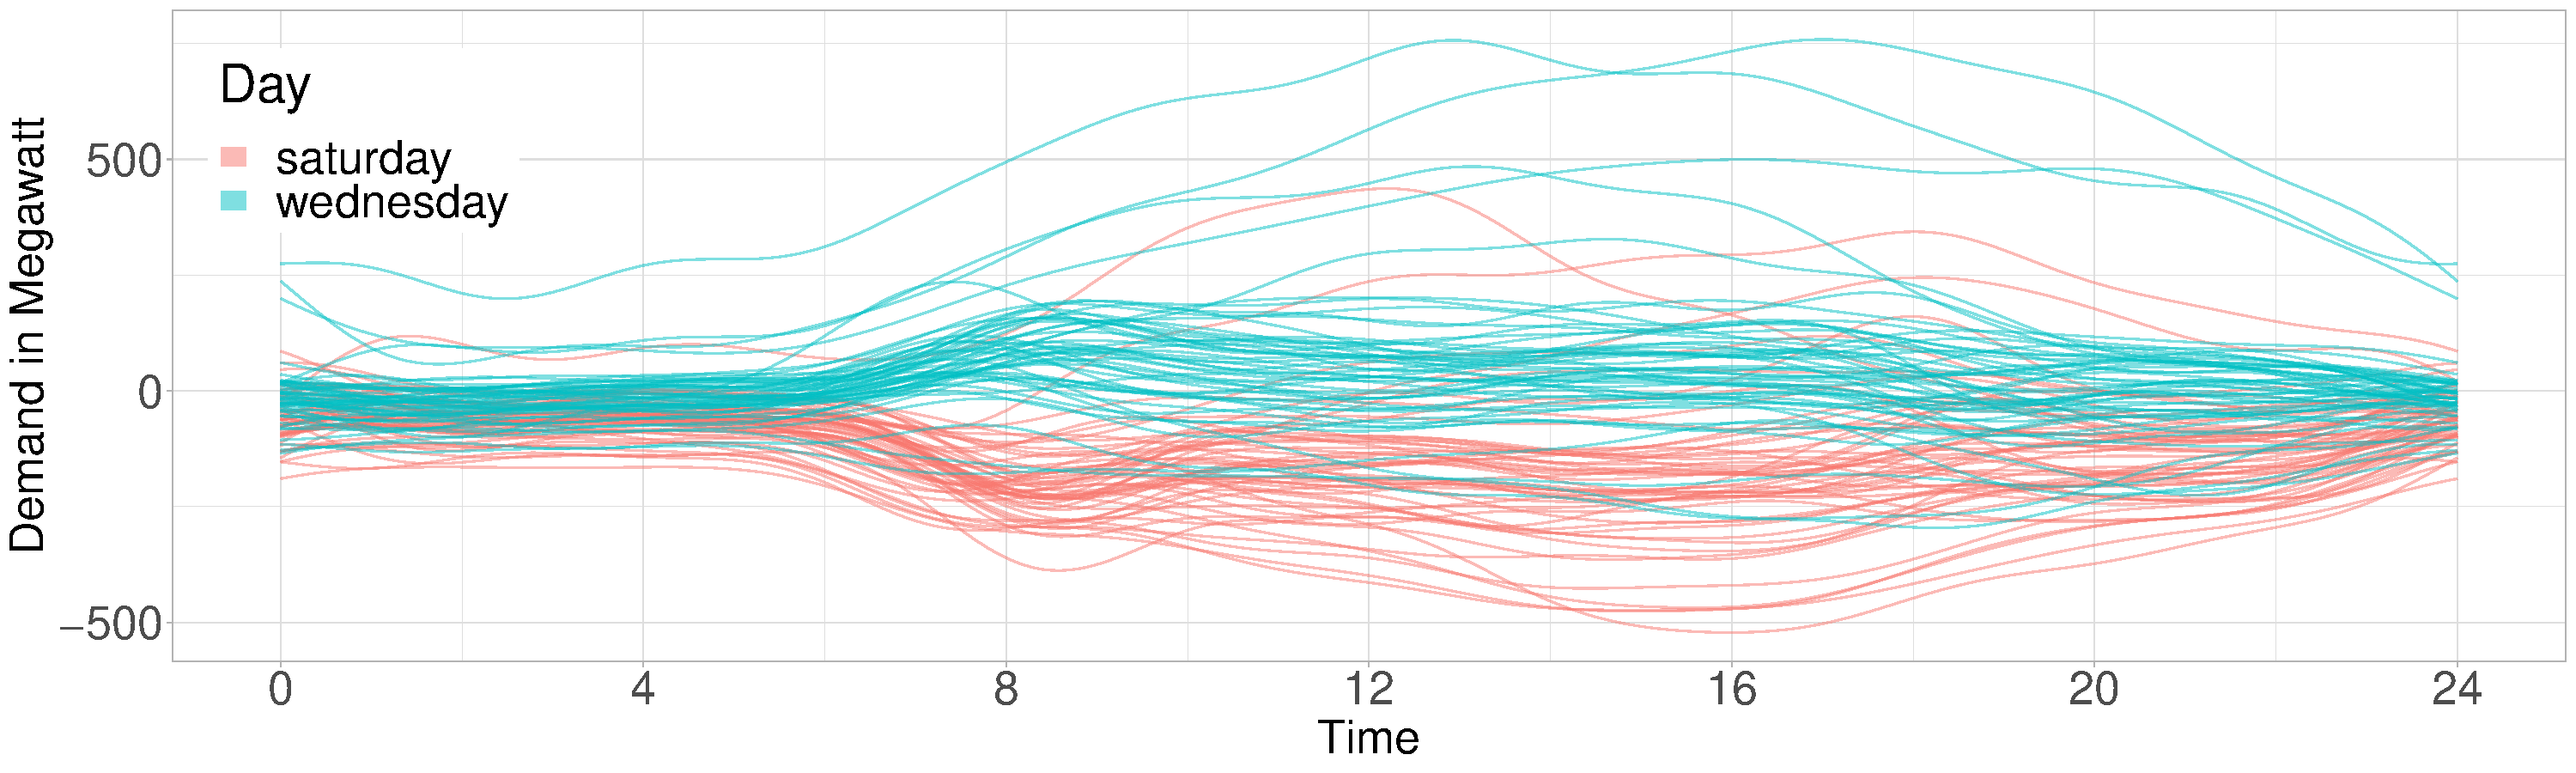
\includegraphics[width=1.1\textwidth]{../Graphics/electricity_demand_curves_cleaned.PDF}
			}
				\caption{Pre-Processed Electricity Demand in Adelaide}
				\label{electricity_demand_cleaned}
			\end{figure}
			As Figure \ref{electricity_demand_cleaned} already shows a considerable mean shift, that is more extreme than those shown in the simulation, it is expected that the test will pick up on these differences. Additionally, as the sample size is considerably bigger in this scenario with 478 observations  and 1404 observations corresponding to Saturdays and working days respectively. As the power of permutation tests is typically quite sensitive to the sample size, this is another reason to assume strong power against the apparent violation of the null hypothesis.
			Using the same decision rules as in the simulation study leads to the following rejection decisions.
			\begin{table}[H]
				\centering
				\begin{tabular*}{\textwidth}{l @{\extracolsep{\fill}} c @{\extracolsep{\fill}} c}
					\toprule
					\textbf{Test}	&$\left(\alpha_{\tau}, \alpha_{\nu}\right) $ &\textbf{Rejection of the Null?} \\
					\midrule
					Means-Test		& $\alpha_{\nu} = 0.05$		& \checkmark \\
					CvM-Test 		& $\alpha_{\tau} = 0.05$	& \checkmark \\
					\midrule
					Combined		& (0.04, 0.01)				& \checkmark	\\
									& (0.03, 0.02)				& \checkmark	\\
									& (0.025, 0.025)			& \checkmark	 \\
									& (0.02, 0.03)				& \checkmark	\\
									& (0.01, 0.04)				& \checkmark	\\
					\bottomrule
				\end{tabular*}
				\caption{Results of the Test from \cite{bugni_permutation_2021}}
			\end{table}
			As mentioned before, these rejections of the null hypothesis are unsurprising when looking at the curves generated for the different days in the data cleaning step. There, it was obvious that the difference in mean alone was stark between workdays and Saturdays. Therefore, it was expected for the mean-based test to find the violation of the null hypothesis in this comparatively large sample problem. Due to the large differences in mean alone, it is also unsurprising that the CvM type test picked up on the violation.
			This application can therefore serve more as a real-world proof of concept for the test. In reality, most scenarios where applying this test will be interesting will be less obvious in the violation of the null hypothesis. Especially violations created by differing persistence structures will typically be difficult to identify. Therefore, applying this test to more challenging settings would be interesting. Section \ref{pot_appl} presents a small selection of settings that might be interesting for further application of the procedures described in this thesis.
	
	\section{Outlook}\label{Outlook}
		This Outlook section will present some problems that came up during the process of writing this thesis that might be interesting to study in further research. Additionally, it presents some ideas for simulations that could improve the understanding of methods such as CvM type tests in a functional data setting and presents real-world scenarios that might be interesting applications for the methods introduced in this thesis.
		
		\subsection{Potential Problems}
			The results presented in this thesis give a good impression of the possibilities of the method developed in \cite{bugni_permutation_2021}. However, there are also potential problems that should not go unnamed.
			
			\paragraph{Implementation\\}
				One source of problems that might influence the results of the simulations is the specific implementation that was used to perform the simulation. As addressed in Section \ref{problem_curve_fitting}, seemingly small choices such as whether to use a functional basis to represent the observations can have a significant impact on the performance and reliability of the simulation and its results.
				
			\paragraph{Definition of $\mathbb{L}_2[0,1]$ \\}
				As mentioned multiple times in this thesis, \cite{bugni_permutation_2021} use an unconventional definition of $\mathbb{L}_2[0,1]$ that makes some theoretical considerations of the methods considerably harder. Therefore, questions such as how this convention interacts with the type of measures that is used in the CvM type test should be studied further. 
				
			\paragraph{Potential Gap in a Proof\\}
				Parts of the proofs presented in the supplementary material to \cite{bugni_permutation_2021} hinge on the assumption that the space of square-integrable functionals with respect to the chosen measure $\mu$ is a separable Hilbert space. In many cases square-integrability is a property that easily allows to show the properties of separable Hilbert spaces. However, as it is not shown in the proofs to be a general property or follow from the type of measure the authors construct, they seem to be incomplete and further consideration should be given to fill these gaps.
	
		\subsection{Theoretical Extensions}
			\paragraph{Variants of the Test based on different Norms\\}
			In the classical scalar setting one common alternative to the CvM test is the Kolmogorov-Smirnov test. Instead of using the squared distance between to objects, it is based on the supremum norm. It could therefore be used to construct an alternative test statistic in the following way. 
			\begin{equation}
				\tau^{\textit{KS}}_{m,n} = \sup_{z \in \mathbb{L}_2[0,1]} \vert \hat{F}_n(z) - \hat{G}_m(z) \vert
			\end{equation}
			Similar to the approximation by Monte-Carlo integration in the main case, this would have to be approximated in an actual implementation. One obvious approach being the following, where $Z_i \stackrel{\text{i.i.d.}}{\sim} Z$ and $Z$ is a random function as described in Section \ref{mu}.
			\begin{equation}
				\hat{\tau}^{\textit{KS}}_{m,n} = \max_{i = 1, \dots, H}\left\{\vert \hat{F}_n(Z_i) - \hat{G}_m(Z_i) \vert \right\}
			\end{equation}
			Other variants could be used in a similar way leading to a plethora of possible test statistics. It would be interesting to compare them both from a theoretical perspective and using simulations to assess their power in different scenarios.
		
		\subsection{Possible Further Simulations}
			After studying the method developed by \cite{bugni_permutation_2021} in detail there are a few points that might be interesting for further research. In the following I name a few that could be very interesting extension to this thesis.
			
			\paragraph{Comparing different Functional Bases\\} 
			For the construction of the measure and potentially also for fitting the observations a functional basis is used. Even in settings, where observations are not fitted using methods like this, the basis that is used to construct the measure might influence the properties of the test. From a theoretical perspective, the test is only justified for complete orthonormal bases, but it would be interesting to study its properties in simulations even for bases that do not have these properties, such as for example a b-spline basis.
		
			\paragraph{Comparing choices of $w(t)$ and  $\left(\rho_i\right)_{i = 1, the \dots, K}$\\}
			In this thesis I only perform simulations for one intuitive choice of $w(t)$ and $\left(\rho_i\right)_{i = 1, \dots, K}$. It seems reasonable to assume that these parameter choices could have a significant impact on the performance of the method and it would therefore be interesting to compare different choices in a structured framework.
			
			\paragraph{Less restrictive Distributions of Fourier Coefficients\\}
			The measures constructed as part of the CvM type test described in this thesis drew their Fourier coefficients using independently distributed error terms. Even though this leads to a convenient implementation, using measures induced by random variables generated using error terms with a more general dependence structure might be beneficial to increase the power against specific alternatives. It would therefore be interesting to study the influence on the measure on the power of the test in more general settings both from a theoretical perspective and using simulations. 
		
			\paragraph{Simulations for Unbalanced Sample Sizes\\}
			The simulations in this thesis only dealt with settings in which both the reference sample and the second sample contained the same number of curves. Even though there is no obvious theoretical reason for unbalanced sample sizes to influence the power of the test meaningfully, it would be interesting to study settings with unbalanced sample sizes in further simulations.		
			
			\paragraph{Comparing Implementations using different orders of Operations\\}
			As described in Sections \ref{persistence_test} and \ref{sim_persistence}, the actual implementation could be highly important for the properties of the proposed test for persistence alternatives. This thesis only provides two heuristic simulations to compare the performance of the proposed options due to computational limitations. Therefore, it would be interesting to actually compare these options in further full-scale simulations.
		
		\subsection{Potential Applications}\label{pot_appl}
			As explained in Section \ref{Application}, the chosen setting is suitable to apply the test, but it is more of a showcase then what this method would be used for in reality. Therefore, it would be interesting to apply the method and the variant for persistence alternatives to data that is more fitting. Two examples that could provide interesting applications for this method are listed in the following.
			\begin{itemize}
				\item \textbf{Audio-Curves} and specifically speech recordings are a typical scenario for functional data. The tests described in this thesis could be used to compare samples of recordings of spoken words. One interesting application could be to determine whether a set of recordings was manipulated when there is an appropriate reference sample that is known to be authentic. Especially in the context of computer generated speech imitation, sometimes known as voice deep-fakes, a test that could reliably distinguish between original and imitated speech recordings could be highly relevant.
				\item \textbf{Movement-Curves} such as for example curves describing the movement of a runner's legs during a 100m sprint might also be an interesting field for potential applications. Given a reference sample of movement curves of runners with a specific alteration to their movement due to e.g. a sickness, the test might be useful in the context of medical diagnostics.
			\end{itemize}
		
		
	
	\newpage
	\section{Bibliography}
	\printbibliography[heading=none]
	
	\newpage
	\cleardoublepage
	\pagenumbering{roman}
	\setcounter{page}{1}
	\section{Appendix}
	
		\subsection{Informal Intuition}\label{Intuition}
			For potential readers unfamiliar with functional data analysis and permutation testing, the initial hurdle of reading this thesis without any intuitive understanding might be high. Therefore, this short informal introduction should serve as a primer that gives an intuitive idea about the following questions.
			\begin{multicols}{2}
				\begin{enumerate}
					\item What setting are we in?
					\item What do we want to test?
					\item How do we want to test it?
					\item Why should I care?
				\end{enumerate}
			\end{multicols}
			By choice, this section will \textbf{not} be formal and it will \textbf{not} be precise so as not to introduce too much detail that could hinder an intuitive understanding.\\
			
			Answering question one is relatively simple. This thesis deals with a statistical problem where observations are continuously observed curves. But what does that mean intuitively? One scenario that is easy to imagine is a curve over time for some variable such as speed: When driving a car at the 24-hour race at Le-Mans, it has a speed at every point in time during the race - for example, $155.3$ km/h at 2 hours, 33 minutes and 7 seconds after the race has started. Observations in the sense of this thesis are similar to this curve: at every value of $x$ in some closed interval $[a,b] \subset \mathbb{R}$, we observe a value $y$.\\
			
			Question two is also simple. We want to test if two samples of curves are similar in a specific way. As in many statistical problems, we interpret the observations as realizations of some random variable. The only difference is that these observations are curves. So we can ask the question of whether the curves in the two samples are dissimilar enough for us to say confidently that they were not generated by the same random variable. 
			Staying with the example of Le-Mans, we could have two identical cars with two equally skillful drivers collect 24-hour speed curves for the next ten years. We do this to determine if two different types of fuel change the way the cars act on the track. We now have two samples, each containing 3650 speed curves in this hypothetical scenario. 
			We want to test statistically whether changing the fuel made any difference.\\
			
			Question three is more difficult. Therefore, let's give the correct intuition by answering a simpler question instead. Let us return to the scalar setting for a moment - each observation is just a real number $x \in \mathbb{R}$ again. We want to determine whether two samples are different enough for us to confidently say: ``These samples are too dissimilar to be generated by the same random variable.'' If you have some statistical knowledge, your first intuition might be to perform a Kolmogoroff-Smirnov, CvM or Anderson-Durbin test. However, let us take one step back first and think about a more general idea.\\
			
			From an intuitive point of view, if the two samples were generated by the same random variable, the effect of randomly switching observations between the samples should be small. Formalizing this idea leads to the concept of permutation tests. By randomly permuting the samples and calculating a chosen test statistic on the permuted samples, one could derive a distribution for the test statistic that can be used for testing. If the test statistic calculated on the non-permuted samples is comparatively extreme, this could be an indicator that the samples were not generated by the same random variable.\\
			
			Why you should care about this is the hardest question. I care about it because it is cool from a mathematical perspective. Nevertheless, if you care about real-life problems, there are also good reasons to be interested. Economic data is being observed at increasing frequencies as technology improves. Many problems that were previously low dimensional due to data constraints or suitable for classical time series methods are becoming more complex as methodological challenges such as high-dimensionality and extreme correlation of neighboring observations arise. Functional data analysis is a comparatively new approach to many of these problems that transform some of these problems into strengths by acknowledging the functional structure of the underlying processes. Permutation tests are also comparatively new, at least in our ability to apply them on a larger scale.
			
		\subsection{$\mathbb{L}_2[0,1]$ as defined in \cite{bugni_permutation_2021}}\label{deviation}
		To distinguish between the typical case presented in the previous section, let $\mathbb{L}_2[0,1]$ denote the Hilbert space of square-integrable functions and $\mathbb{L}^{*}_2[0,1]$ the square-integrable functions under the the convention from \cite{bugni_permutation_2021}.\\
		
		Using $\mathbb{L}^{*}_2[0.1]$ creates some interesting theoretical challenges, as the resulting object is in fact not a Hilbert space. To understand the theoretical problems that can occur, I first introduce some additional concepts to illustrate the challenges.
		\begin{definition}[Norm and Seminorm]
			A function $p : \mathbb{V} \rightarrow \mathbb{F}$ on a vector space $\mathbb{V}$ over a field $\mathbb{F}$ is called a norm if the following four conditions hold for all $v,u \in \mathbb{V}$ and $s \in \mathbb{F}$.
			\begin{multicols}{2}
				\begin{enumerate}
					\item $p(v + u) \leq p(v) + p(u)$
					\item $p(sv) = |s| p(v)$
					\item $p(v) \geq 0$
					\item $p(v) = 0 \implies v = 0$
				\end{enumerate}
			\end{multicols}
			If $p : \mathbb{V} \rightarrow \mathbb{F}$ fulfills only properties (1) to (3) it is called a seminorm.
		\end{definition}
		
		In the same way a norm induces a distance on its corresponding normed vectorspace, a seminorm $p$ induces a so-called pseudometric $d$. It is given by $d(v,u) = p(u-v)$.
		
		{\color{red} This is from Wikipedia!!!}
		\begin{definition}[Pseudometric Space]
			A pseudometric space $\left(X, d\right)$ is a set $X$ together with a function $d:X\times X \rightarrow \mathbb{R}_{\geq 0}$, such that $\forall x,y,z \in X$ the following properties hold.
			\begin{multicols}{2}
				\begin{enumerate}
					\item $d(x,x) = 0$
					\item $d(x,y) = d(y,x)$
					\item $d(x,z) \leq d(x,y) + d(y,z)$
				\end{enumerate}
			\end{multicols}
			Therefore, deviating from a metric space, two distinct points in a pseudometric space can have a distance of zero $d(x,y) = 0$ for $x \neq y$.
		\end{definition}
		
		That $\mathbb{L}^{*}_2[0,1]$ is not a Hilbert space becomes clear, when checking the for the properties of the norm induced by the inner product $\| v \| = \sqrt{\langle v, v\rangle}$.
		One of the properties that has to be fulfilled by a norm is $\| v \| = 0 \Longleftrightarrow v = 0$.			
		Let $f:[0,1] \rightarrow \mathbb{R}$ be given by $f(x) = \mathbbm{1}\left[x = 0.5\right]$. Then we can evaluate the following expression to create a contradiction to the norm properties.
		\begin{equation}
			\| f \| = \sqrt{\langle f, f\rangle} = \sqrt{\int_{0}^{1} \left[f(t)\right]^2\mathrm{d}t } = 0
		\end{equation}
		As $f$ is not the zero element of this space, this is a violation of positive definiteness. Positive definiteness applied to the case at hand, states that $\forall v \in \mathbb{L}_2[0,1] \| v \| = 0 \implies v(x) = 0 \quad \forall x \in [0,1]$  $\forall v \in $. Instead, $\| v \| = \sqrt{\langle v, v\rangle}$ is a seminorm and the defined space should more correctly be treated as a pseudometric space.\\
		
		{\color{red} This is from Wikipedia!!!}
		\begin{definition}[Hausdorff Space]
			A Hausdorff space is a topological space where for any two distinct points $x$ and $y$, there exist a neighborhood $U$ of $x$ and a nieghborhood $V$ of $y$ such that $U$ and $V$ are disjoint. This property is also called neighborhood-separability.
		\end{definition}
		
		One problem of $\mathbb{L}^{*}_2[0,1]$ is, that if we give the space the topology induced by the obvious seminorm, the resulting space would not be Hausdorff. Thus, limits in the later part of \cite{bugni_permutation_2021} would not be defined.
		A second problem is, that it is not clear how a Schauder basis would be defined for a pseudometric space such as $\mathbb{L}^{*}_2[0,1]$ and that typical existence results for orthonormal bases might not be available.\\				
		
		\subsection{Asymptotic Distribution of the Cram\'{e}r-von Mises Test}\label{asymp_CvM}
			As shown by \cite{rosenblatt_limit_1952} and \cite{fisz_result_1960}, under the null hypothesis that both samples were independently generated by random variables sharing the same distribution function, we can find the following limiting distribution of $C_{m,n}$.
			\begin{equation}
				\begin{split}
					C_{m,n} &\xrightarrow{\text{d}} \int_{0}^{1} \left(Z(u) + \left(1 + \lambda\right)^{-\frac{1}{2}} f(u) - \left[\frac{\lambda}{1+\lambda}\right]^{\frac{1}{2}}g(u)\right)^2 \mathrm{d}u \\
					\text{as} \quad &n \rightarrow \infty, \quad m \rightarrow \infty, \quad \frac{n}{m} \rightarrow \lambda \in \mathbb{R}
				\end{split}
			\end{equation}
			Here, $f(u)$ and $g(u)$ are the probability density functions of the corresponding random variables and $Z(u)$ is a Gaussian stochastic process with the following properties.
			\begin{itemize}
				\item $\mathbb{E}\left[Z(u)\right] = 0 \quad \forall u \in [0,1]$
				\item $Cov\left(Z(u), Z(v)\right) = \min(u,v) - uv \quad \forall u,v \in [0,1]$
			\end{itemize}
		
		\subsection{Proof from \cite{hoeffding_large-sample_1952}}\label{hoeffding}
			\paragraph{Theorem as stated in \cite{lehmann_testing_2005} \\}
			Suppose $X^N$ has distribution $P_N$ in $\mathcal{X}_N$, and $G_N$ is a finite group of transformations from $\mathcal{X}_N$ to $\mathcal{X}_N$. Let $\mathcal{G}_N$ be a random variable that is uniform on $G_N$. Also let $\mathcal{G}_N'$ have the same distribution as $\mathcal{G}_N$, with $X^N$, $\mathcal{G}_N$, and $\mathcal{G}_N'$ mutually independent. Suppose, under $P_N$,
			\begin{equation}\label{convergence_hypo}
				\left(T_N(\mathcal{G}_N X^N), T_N(\mathcal{G}_N' X^N)\right) \rightarrow_d (T, T'),
			\end{equation}
			where $T$ and $T'$ are independent, each with common cumulative distribution function $R(t)$. Then, under $P_N$,
			\begin{equation}
				\hat{R}_N(t) \rightarrow_P R(t)
			\end{equation}
			for every $t$ which is a continuity point of $R(t)$.
		
			\paragraph{Proof as presented in \cite{lehmann_testing_2005}\\}
			Let $t$ be a continuity point of $R(t)$. Then, 
			\begin{equation}
				\mathbb{E}_{P_N}\left[\hat{R}_N(t)\right] = P_N\left[T_N(\mathcal{G}_NX^N) \leq t\right] \rightarrow R(t),
			\end{equation}
			by the convergence hypothesis shown in Equation \ref{convergence_hypo}. It therefore suffices to show that $\textit{Var}_{P_N}\left[\hat{R}_N(t)\right] \rightarrow 0$ or, equivalently, that
			\begin{equation}
				\mathbb{E}_{P_N}\left[\hat{R}_N^2(t)\right] \rightarrow R^2(t).
			\end{equation}
			But, 
			\begin{equation}
				\begin{split}
					\mathbb{E}_{P_N}\left[\hat{R}_N^2(t)\right] &= \frac{1}{M_N^2}\sum_{g \in G_N}\sum_{g' \in G_N} P_N\left[T_N(gX^N) \leq t \ \land \ T_N(g'X^N) \leq t\right] \\
					&= P_N\left[T_N(\mathcal{G}_NX^N) \leq t \ \land \ T_N(\mathcal{G}_N'X^N) \leq t\right] \rightarrow R^2(t),
				\end{split}
			\end{equation}
			again by the convergence hypothesis. Hence $\hat{R}_N(t) \rightarrow R(t)$ in $P_N$ probability.
			
		\subsection{Argument for Finiteness}\label{finiteness}
		The following argument can be made concerning the finiteness of the mean.
		\begin{equation}
			\begin{split}
				& \hat{F}_n(z) \in [0,1] 	\land \hat{G}_m(z) \in [0,1] \implies \left[\hat{F}_n(z) - \hat{G}_m(z)\right]^2 \in [0,1] \quad \forall z \in \mathbb{L}_2[0,1]\\
				& \int_{\mathbb{L}_2[0,1]} 1 \ \mathrm{d}\mu(z) = 1 \land \int_{\mathbb{L}_2[0,1]} 0 \ \mathrm{d}\mu(z) = 0 \implies \int_{\mathbb{L}_2[0,1]}\left[\hat{F}_n(z) - \hat{G}_m(z)\right]^2 \mathrm{d}\mu(z) \in [0,1]
			\end{split}
		\end{equation}			 
		The same argument can be made concerning the variance.
		\begin{equation}the 
			\begin{split}
				& \left(\left[\hat{F}_n(z) - \hat{G}_m(z)\right]^2 \in [0,1] \quad \forall z \in \mathbb{L}_2[0,1]\right) \land \left(\int_{\mathbb{L}_2[0,1]}\left[\hat{F}_n(z) - \hat{G}_m(z)\right]^2 \mathrm{d}\mu(z) \in [0,1] \right)\\
				& \implies \left[ \left[\hat{F}_n(z) - \hat{G}_m(z)\right]^2 - \int_{\mathbb{L}_2[0,1]}\left[\hat{F}_n(z) - \hat{G}_m(z)\right]^2 \mathrm{d}\mu(z) \right]^2 \in [0,1] \ \forall z \in \mathbb{L}_2[0,1]\\
				& \int_{\mathbb{L}_2[0,1]} 1 \ \mathrm{d}\mu(z) = 1 \land \int_{\mathbb{L}_2[0,1]} 0 \ \mathrm{d}\mu(z) = 0 \\
				& \implies \int_{\mathbb{L}_2[0,1]}\left[ \left[\hat{F}_n(z) - \hat{G}_m(z)\right]^2 - \int_{\mathbb{L}_2[0,1]}\left[\hat{F}_n(z) - \hat{G}_m(z)\right]^2 \mathrm{d}\mu(z) \right]^2 \mathrm{d}\mu(z) \in [0,1] \\
			\end{split}
		\end{equation}
	
		\subsection{Derivation of Asymptotic Distribution}\label{asymp_deriv}
			This section presents an adapted proof for the limiting distribution of the CvM permutation test as presented in the supporting information of \cite{bugni_permutation_2021}, additional information was taken from the proof of Theorem 3.1 in \cite{bugni_goodness--fit_2009}.\\
	
			\begin{theorem}\label{asymp_proof}
				Let Assumptions \ref{Ass1} and \ref{mean_existence} be fulfilled and  and define $\Upsilon(z)$ as in Section \ref{asymp}. Then the following statement holds.
				\begin{equation}
					\tau_{n,m} \rightarrow_d \int_{\mathbb{L}_2[0,1]}\Upsilon^2(z) \mathrm{d}\mu(z)
				\end{equation}
			\end{theorem}
			
			Additionally, it is useful to prove the following Lemmas taken from the supporting information of \cite{bugni_permutation_2021} before proving the main point.
			Define the following objects
				\begin{equation}
					W_i(t) = \mathbbm{1}\left[i \leq n\right] X_i(t) + \mathbbm{1}\left[i > n\right] Y_{i-n}(t)
				\end{equation}
				\begin{equation}
					U_i = \mathbbm{1}\left[i \leq n\right] \frac{N}{n} + \mathbbm{1}\left[i > n\right] \frac{N}{m}
				\end{equation}
				\begin{equation}
					F_{nX}(z) = G(z) + \frac{1}{N}D(z)
				\end{equation}
				for a chosen function $D(z)$ fulfilling $\int_{\mathbb{L}_2[0,1]}D^2(z) \mathrm{d} \mu(z) < \infty$.
			
			\begin{theorem}[Lemma A.3]
				content...
			\end{theorem}
		
			\begin{proof}
				content...
			\end{proof}
		
			\begin{theorem}[Lemma A.4]
				Let Assumptions \ref{Ass1} and \ref{mean_existence} be fulfilled. Then, 
				\begin{equation}
					\frac{1}{\sqrt{N}} \int_{\mathbb{L}_2[0,1]} \left[ \hat{F}_n(z) - \hat{G}_{m}(z) \right] \left\{\psi_k(z)\right\}_{k = 1}^K \mathrm{d}\mu(z)\rightarrow_d \mathcal{N}(\Xi, \Sigma_K)
				\end{equation}
				where 
				\begin{equation}
					\Xi = \int_{\mathbb{L}_2[0,1]}D(z) \left\{\psi_k(z)\right\}_{k = 1}^K \mathrm{d}\mu(z)
				\end{equation}
				and 
				\begin{equation}
					\left(\Sigma_K\right)_{i,j} = \frac{(1 + \lambda)^2}{\lambda} \int_{\mathbb{L}_2[0,1]}\int_{\mathbb{L}_2[0,1]} \left[G(\min(z, 	\tilde{z})) - G(z)G(\tilde{z}))\right] \psi_i(z) \psi_j(\tilde{z}) \mathrm{d}\mu(z) \mathrm{d}\mu(\tilde{z})
				\end{equation}
				where $\min(z, \tilde{z})$ is defined as in Section \ref{asymp}.
			\end{theorem}
		
			\begin{proof}
				We have
				\begin{equation}\label{piece1}
					\begin{split}
						\frac{1}{\sqrt{N}}\left[F(z) - G(z)\right] &= \frac{1}{\sqrt{N}} \Bigg[ \sum_{i = 1}^{N} U_i \mathbbm{1}\left[W_i(t) \leq z(t) \ \forall t \in [0,1]\right] \Bigg]
					\end{split}
				\end{equation}
				{\color{red} Hier Zwischenschritt ergaenzen}\\
				For any $K = 1,2,3,\dots$
				\begin{equation}\label{piece2}
						\frac{1}{\sqrt{N}} \sum_{i = 1}^{N} U_i \bigg\{ \int_{\mathbb{L}_2[0,1]} \mathbbm{1}\left[W_i(t) \leq z(t) \ \forall t \in [0,1] \right] \psi_k(z) \mathrm{d} \mu(z) - \mu_{i,N,k}\bigg\}_{k = 1}^K  \rightarrow \mathcal{N}(0_K, \Sigma_K)
				\end{equation}
				where
				\begin{equation}
					\mu_{i,N,k} = \mathbbm{1}\left[i \leq n\right] \int_{\mathbb{L}_2[0,1]} F_{nX}(z) \psi_k(z) \mathrm{d} \mu(z) + 
					\mathbbm{1}\left[i > n\right] \int_{\mathbb{L}_2[0,1]} G(z) \psi_k(z) \mathrm{d} \mu(z)
				\end{equation}
				Additionally,
				\begin{equation}\label{piece3}
					\frac{1}{\sqrt{N}} \left[ \sum_{i = 1}^{N} U_i \mu_{i,N,k}\right] = \frac{1}{\sqrt{N}} \int_{\mathbb{L}_2[0,1]} D(z) \psi_k(z) \mathrm{d}\mu(z)
				\end{equation}
				The Lemma holds by Equations \ref{piece1}, \ref{piece2} and \ref{piece3}.
			\end{proof}
		
		\begin{proof}[Theorem \ref{asymp_proof}]
			Let $\left(\psi_k\right)_{k \in \mathbb{N}}$ be a complete orthonormal basis of $\mathbb{L}_2(\mu)$ where $\mathbb{L}_2(\mu)$ denotes the Hilbert space of functionals on $\mathbb{L}_2[0,1]$ that are square-integrable with respect to $\mu$. Using a countable basis is only possible if $\mathbb{L}_2(\mu)$ is a separable Hilbert space, which the original authors do not show.\\
			
			For any $z(t) \in \mathbb{L}_2[0,1]$ define:
			\begin{equation}
				H_N(z) = \frac{1}{N} \left[\sum_{i = 1}^{n} \frac{N}{n} \mathbbm{1}\left[X_i(t) \leq z(t)\ \forall t \in [0,1]\right]
				+ \sum_{i = 1}^{m} \frac{N}{m} \mathbbm{1}\left[Y_i(t) \leq z(t)\ \forall t \in [0,1]\right]\right]
			\end{equation} 
			Then,
			\begin{equation}
				\tau_{n,m} = \int_{\mathbb{L}_2[0,1]} H_N^2(z) \mathrm{d}\mu(z)
			\end{equation}
			For any positive integer $K$, define the following objects.
			\begin{multicols}{2}
				\noindent
				\begin{equation*}
					H_{N,K1}(z) = \sum_{k = 1}^{K} c_{N,k}\psi_k(z)
				\end{equation*}
				\begin{equation}
					H_{N,K2}(z) = \sum_{k = K=1}^{\infty} c_{N,k}\psi_k(z)
				\end{equation}
			\end{multicols}
			where
			\begin{equation}
				c_{N,k} = \int_{\mathbb{L}_2[0,1]} H_N(z) \psi_k(z) \mathrm{d}\mu(z)
			\end{equation}
		and therefore
		\begin{equation}
			H_N(z) = \sum_{k = 1}^{\infty} c_{N,k}\psi_k(z) = H_{N,K1}(z) + H_{N,K2}(z).
		\end{equation}
		Similarly, define
		\begin{multicols}{2}
			\noindent
			\begin{equation*}
				\tau_{N,K1} = \int_{\mathbb{L}_2[0,1]} 	H_{N,K1}^2(z) \mathrm{d}\mu(z) = \sum_{k = 1}^{K} c_{N,k}^2
			\end{equation*}
			\begin{equation}
				\tau_{N,K2} = \int_{\mathbb{L}_2[0,1]} 	H_{N,K2}^2(z) \mathrm{d}\mu(z) = \sum_{k = K+1}^{\infty} c_{N,k}^2
			\end{equation}
		\end{multicols}
		and 
		\begin{multicols}{2}
			\noindent
			\begin{equation*}
				\Upsilon_{N,K1}(z) = \int_{\mathbb{L}_2[0,1]} b_k \psi_k(z) \mathrm{d}\mu(z) = \sum_{k = 1}^{K} c_{N,k}^2
			\end{equation*}
			\begin{equation}
				\Upsilon_{N,K2}(z) = \int_{\mathbb{L}_2[0,1]} b_k \psi_k(z) \mathrm{d}\mu(z) = \sum_{k = K+1}^{\infty} c_{N,k}^2
			\end{equation}
		\end{multicols}
		where
		\begin{equation}
			b_k = \int_{\mathbb{L}_2[0,1]}\Upsilon(z) \psi_k(z) \mathrm{d} \mu(z)
		\end{equation}
		and thus 
		\begin{equation}
			 \Upsilon(z) = \Upsilon_{N,K1}(z) + \Upsilon_{N,K2}(z).
		\end{equation}
		Additionally, define
		\begin{multicols}{2}
			\noindent
			\begin{equation*}
				\tau_{K1} = \int_{\mathbb{L}_2[0,1]} 	\Upsilon_{N,K1}^2(z) \mathrm{d}\mu(z)
			\end{equation*}
			\begin{equation}
				\tau_{K2} = \int_{\mathbb{L}_2[0,1]} 	\Upsilon_{N,K2}^2(z) \mathrm{d}\mu(z).
			\end{equation}
		\end{multicols}
		Now, it is necessary to show the following three points.
		\begin{enumerate}
			\item $\tau_{K1} \rightarrow \tau \quad \text{as} \quad K \rightarrow \infty$
			\item $\tau_{N,K1} \rightarrow \tau_{K1} \quad \text{as} \quad N \rightarrow \infty \quad \forall K = 1,2,3, \dots$
			\item $\left(\tau_N - \tau_{N,K1}\right) = \tau_{N,K2} \rightarrow_p 0 \quad \text{as} \quad N \rightarrow \infty \quad \text{followed by} \quad K \rightarrow \infty$
		\end{enumerate}
	
		Concerning point one, the following is easy to see.
		\begin{equation}
			\mathbb{E}[\tau - \tau_{K1}] = \mathbb{E}[\tau_{K2}] = \sum_{k = K+1}^{\infty} \mathbb{E}[b_k^2] \rightarrow 0 \quad \text{as} \quad K \rightarrow \infty \quad \text{because} \quad \mathbb{E}[\Upsilon(z)] \in \mathbb{L}_2(\mu)
		\end{equation}
	
		For point two, define the following objects.
		\begin{multicols}{2}
			\noindent
			\begin{equation*}
				C_{N,K} = \left\{c_{N,k}\right\}_{k=1}^K
			\end{equation*}
			\begin{equation}
				B_{K} = \left\{b_{k}\right\}_{k=1}^K
			\end{equation}
		\end{multicols}
		By Lemma A.4, it follows that $C_{N,K} \rightarrow \mathcal{N}(0, \Sigma_K) \sim B_K$ as $N \rightarrow \infty$ which shows the point.\\
		
		Concerning point three, by Lemma A.3 the following holds.
		\begin{equation}
			\begin{split}
				\mathbb{E}[\tau_{N,K2}] &= \sum_{k = K+1}^{\infty} \mathbb{E}[c_{N,k}^2] \\
				&= \sum_{k = K+1}^{\infty} \Bigg\{ \frac{1}{\sqrt{N}} \left(1 + \frac{m}{n}\right) \int_{z_1 \in \mathbb{L}_2[0,1]} \int_{z_2 \in \mathbb{L}_2[0,1]} D\left[\min(z_1, z_2)\right] \psi_k(z_1) \psi_k(z_2) \mathrm{d}\mu(z_1) \mathrm{d}\mu(z_2) \\
				& - \frac{2}{\sqrt{N}} \left(1 + \frac{m}{n}\right) \left[\int_{z \in \mathbb{L}_2[0,1]} D(z) \psi_k(z) \mathrm{d}\mu(z) \right] \left[\int_{z \in \mathbb{L}_2[0,1]} G(z) \psi_k(z) \mathrm{d}\mu(z) \right] \\
				& + \left(\Sigma_K\right)_{k,k} \left(2 + \frac{n}{m} + \frac{m}{n}\right) \frac{\lambda}{(1 + \lambda)^2} + \frac{1}{N^2} \left[\int_{z \in \mathbb{L}_2[0,1]} D(z) \psi_k(z) \mathrm{d}\mu(z) \right] \sum_{i = 1}^{n}\sum_{j = 1}^{n} \mathbb{E}\left[U_i U_j\right]\Bigg\}
			\end{split}
		\end{equation}
	The last expression is bounded as $n \rightarrow \infty$ for every positive integer $K$, which implies that $\lim_{K \rightarrow \infty} \lim_{N \rightarrow \infty} \mathbb{E}\left[\tau_{N,K2}\right] = 0$. Thus, by Markov's inequality, point three holds.
		\end{proof}
	
			
		\subsection{Multiple Testing}\label{Multiple_Testing}
			When testing statistical hypotheses, it is often helpful or even necessary to test multiple hypotheses independently of each other. One setting where this could be useful is when we want to combine the desirable properties of two tests, as is done by \cite{bugni_permutation_2021}. If the tests do not perfectly depend on each other, this creates a problem relating to the size of the combined test.
			
			\begin{definition}[Family-wise Error Rate]
				The family-wise error rate is the probability of making at least one type-1 error when performing multiple hypothesis tests.
			\end{definition}
		
			The most straightforward correction for this multiple testing problem is the so-called Bonferroni Correction. Introduced by \cite{dunn_multiple_1961}, it is based on Boole's Inequality shown in Equation \ref{bonferroni}, which is sometimes referred to as the Bonferroni Inequality.
			\begin{equation}\label{bonferroni}
				\mathbb{P}\left[\bigcup_{i = 1}^{\infty} A_i\right] \leq \sum_{i = 1}^{\infty} \mathbb{P}\left[A_i\right]
			\end{equation}
			for a countable set of events $A_1, A_2, \dots$.
			This inequality motivates the idea to control the family wise error rate when performing multiple tests by choosing the individual tests' size such that they add up to the desired overall family-wise error rate. However, as tests might be correlated, this could lead to an overall test that is conservative. Still, if little information is known about the correlation structure of the individual test statistics, this idea ensures that the family-wise error rate is at most the sum of the individual test sizes.		

			
		\subsection{Application Data Cleaning}\label{Application_Appendix}
			\subsubsection{Excluded Holidays}
			Holidays that were excluded in the analysis are the following\footnote{These were taken from \url{https://www.australia.gov.au/public-holidays} accessed on 20.05.2022.}: New Year's Day, Australia Day, March Public Holiday, Good Friday, Holy Saturday, Easter Monday, Anzac Day, Queen's Birthday, Labour Day, Christmas Day, Christmas Eve, Christmas Day, Proclamation Day and New Year's Eve. Sunday is nominally a public holiday in South Australia. Easter Sunday is therefore not a special public holiday, but due to its prominence it was excluded in this analysis.
			
			As Australia replaces some holidays that fall on weekends with substitute holidays on the next working day, these were also excluded. For the South Australia, this can occur for New Year's Day, Australia Day, ANZAC Day, Christmas Day, Proclamation Day and New Year's Eve.
		
			\subsubsection{Detrending and Deseasoning Results}\label{detrending}
			Figures \ref{estimates_const_year} and \ref{estimates_months} show the estimates for the coefficient functions as specified in Equation \ref{Data_Cleaning}. These curves were subtracted from the respective observations to eliminate the influence of, for example, the month the data was observed.
			\begin{figure}[H]
				\makebox[\textwidth][c]{
					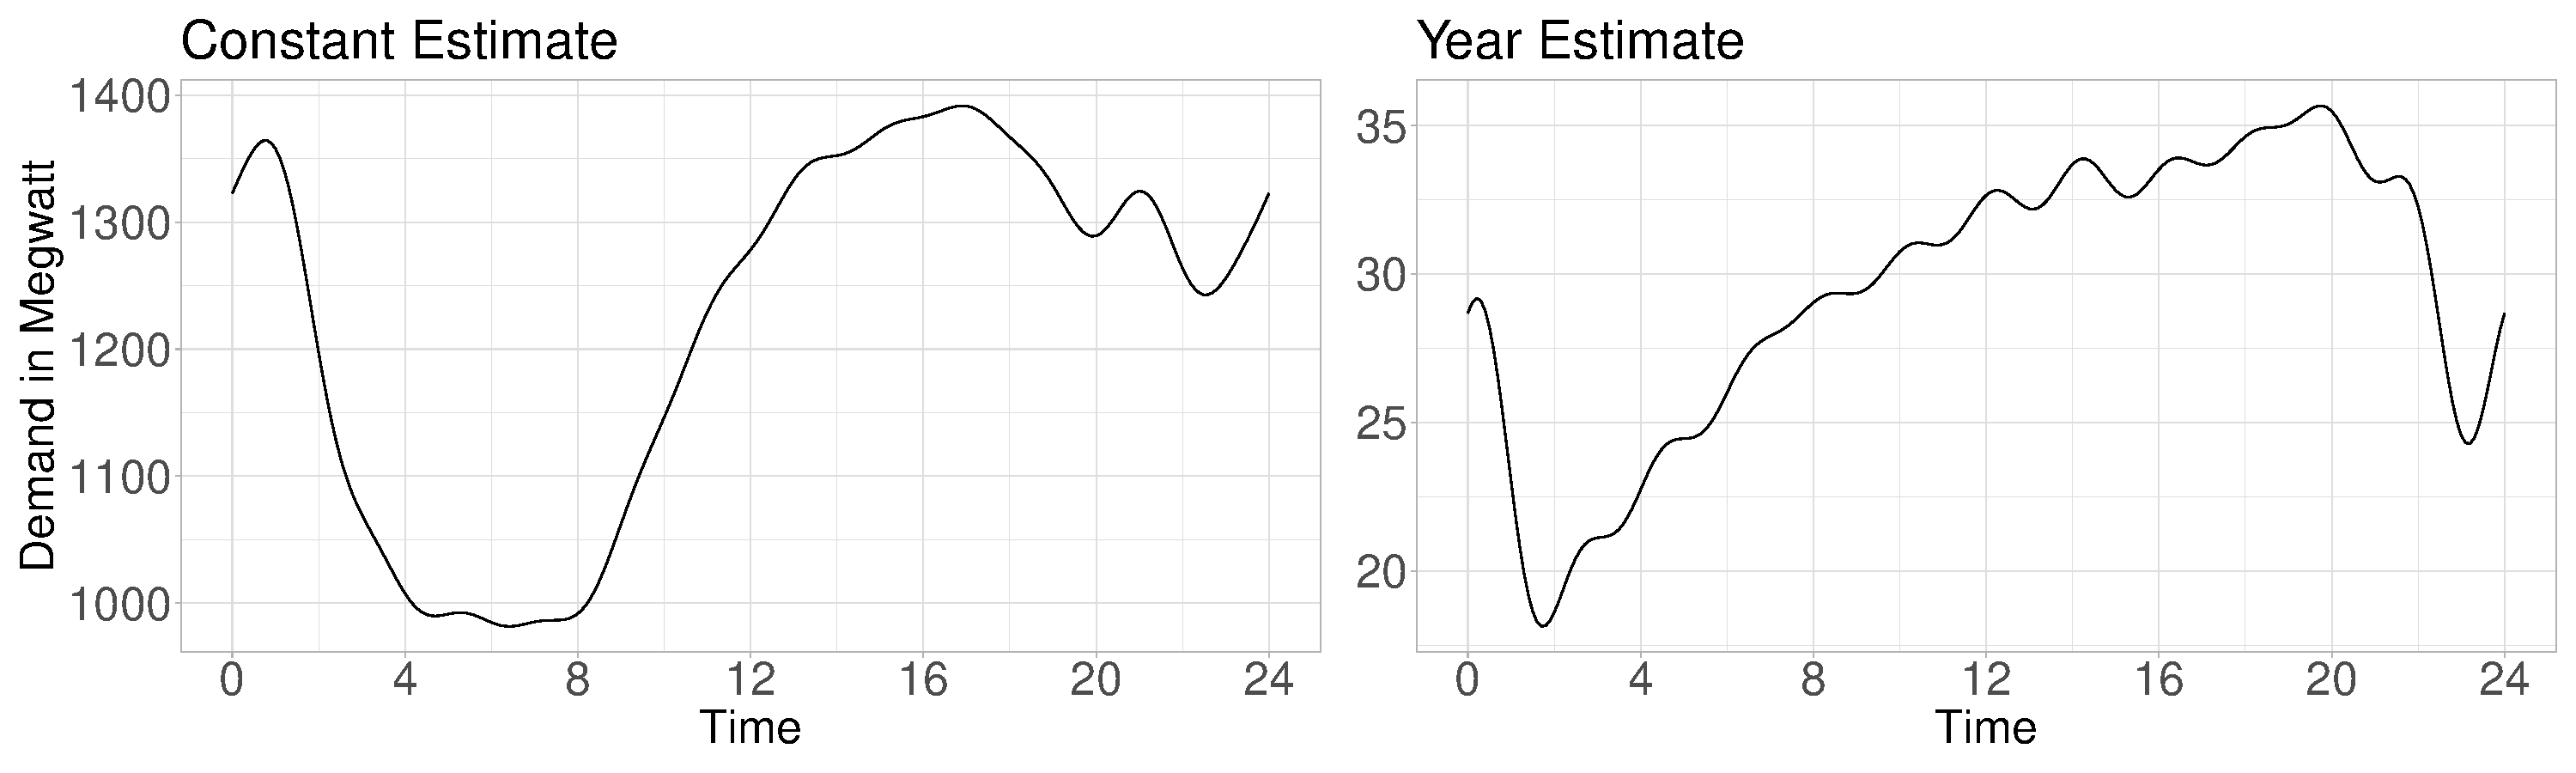
\includegraphics[width=1.1\textwidth]{../Graphics/estimate_const_year.PDF}
				}
				\caption{Estimates for the constant and year}
				\label{estimates_const_year}
			\end{figure}
			
			\begin{figure}[H]
				\makebox[\textwidth][c]{
					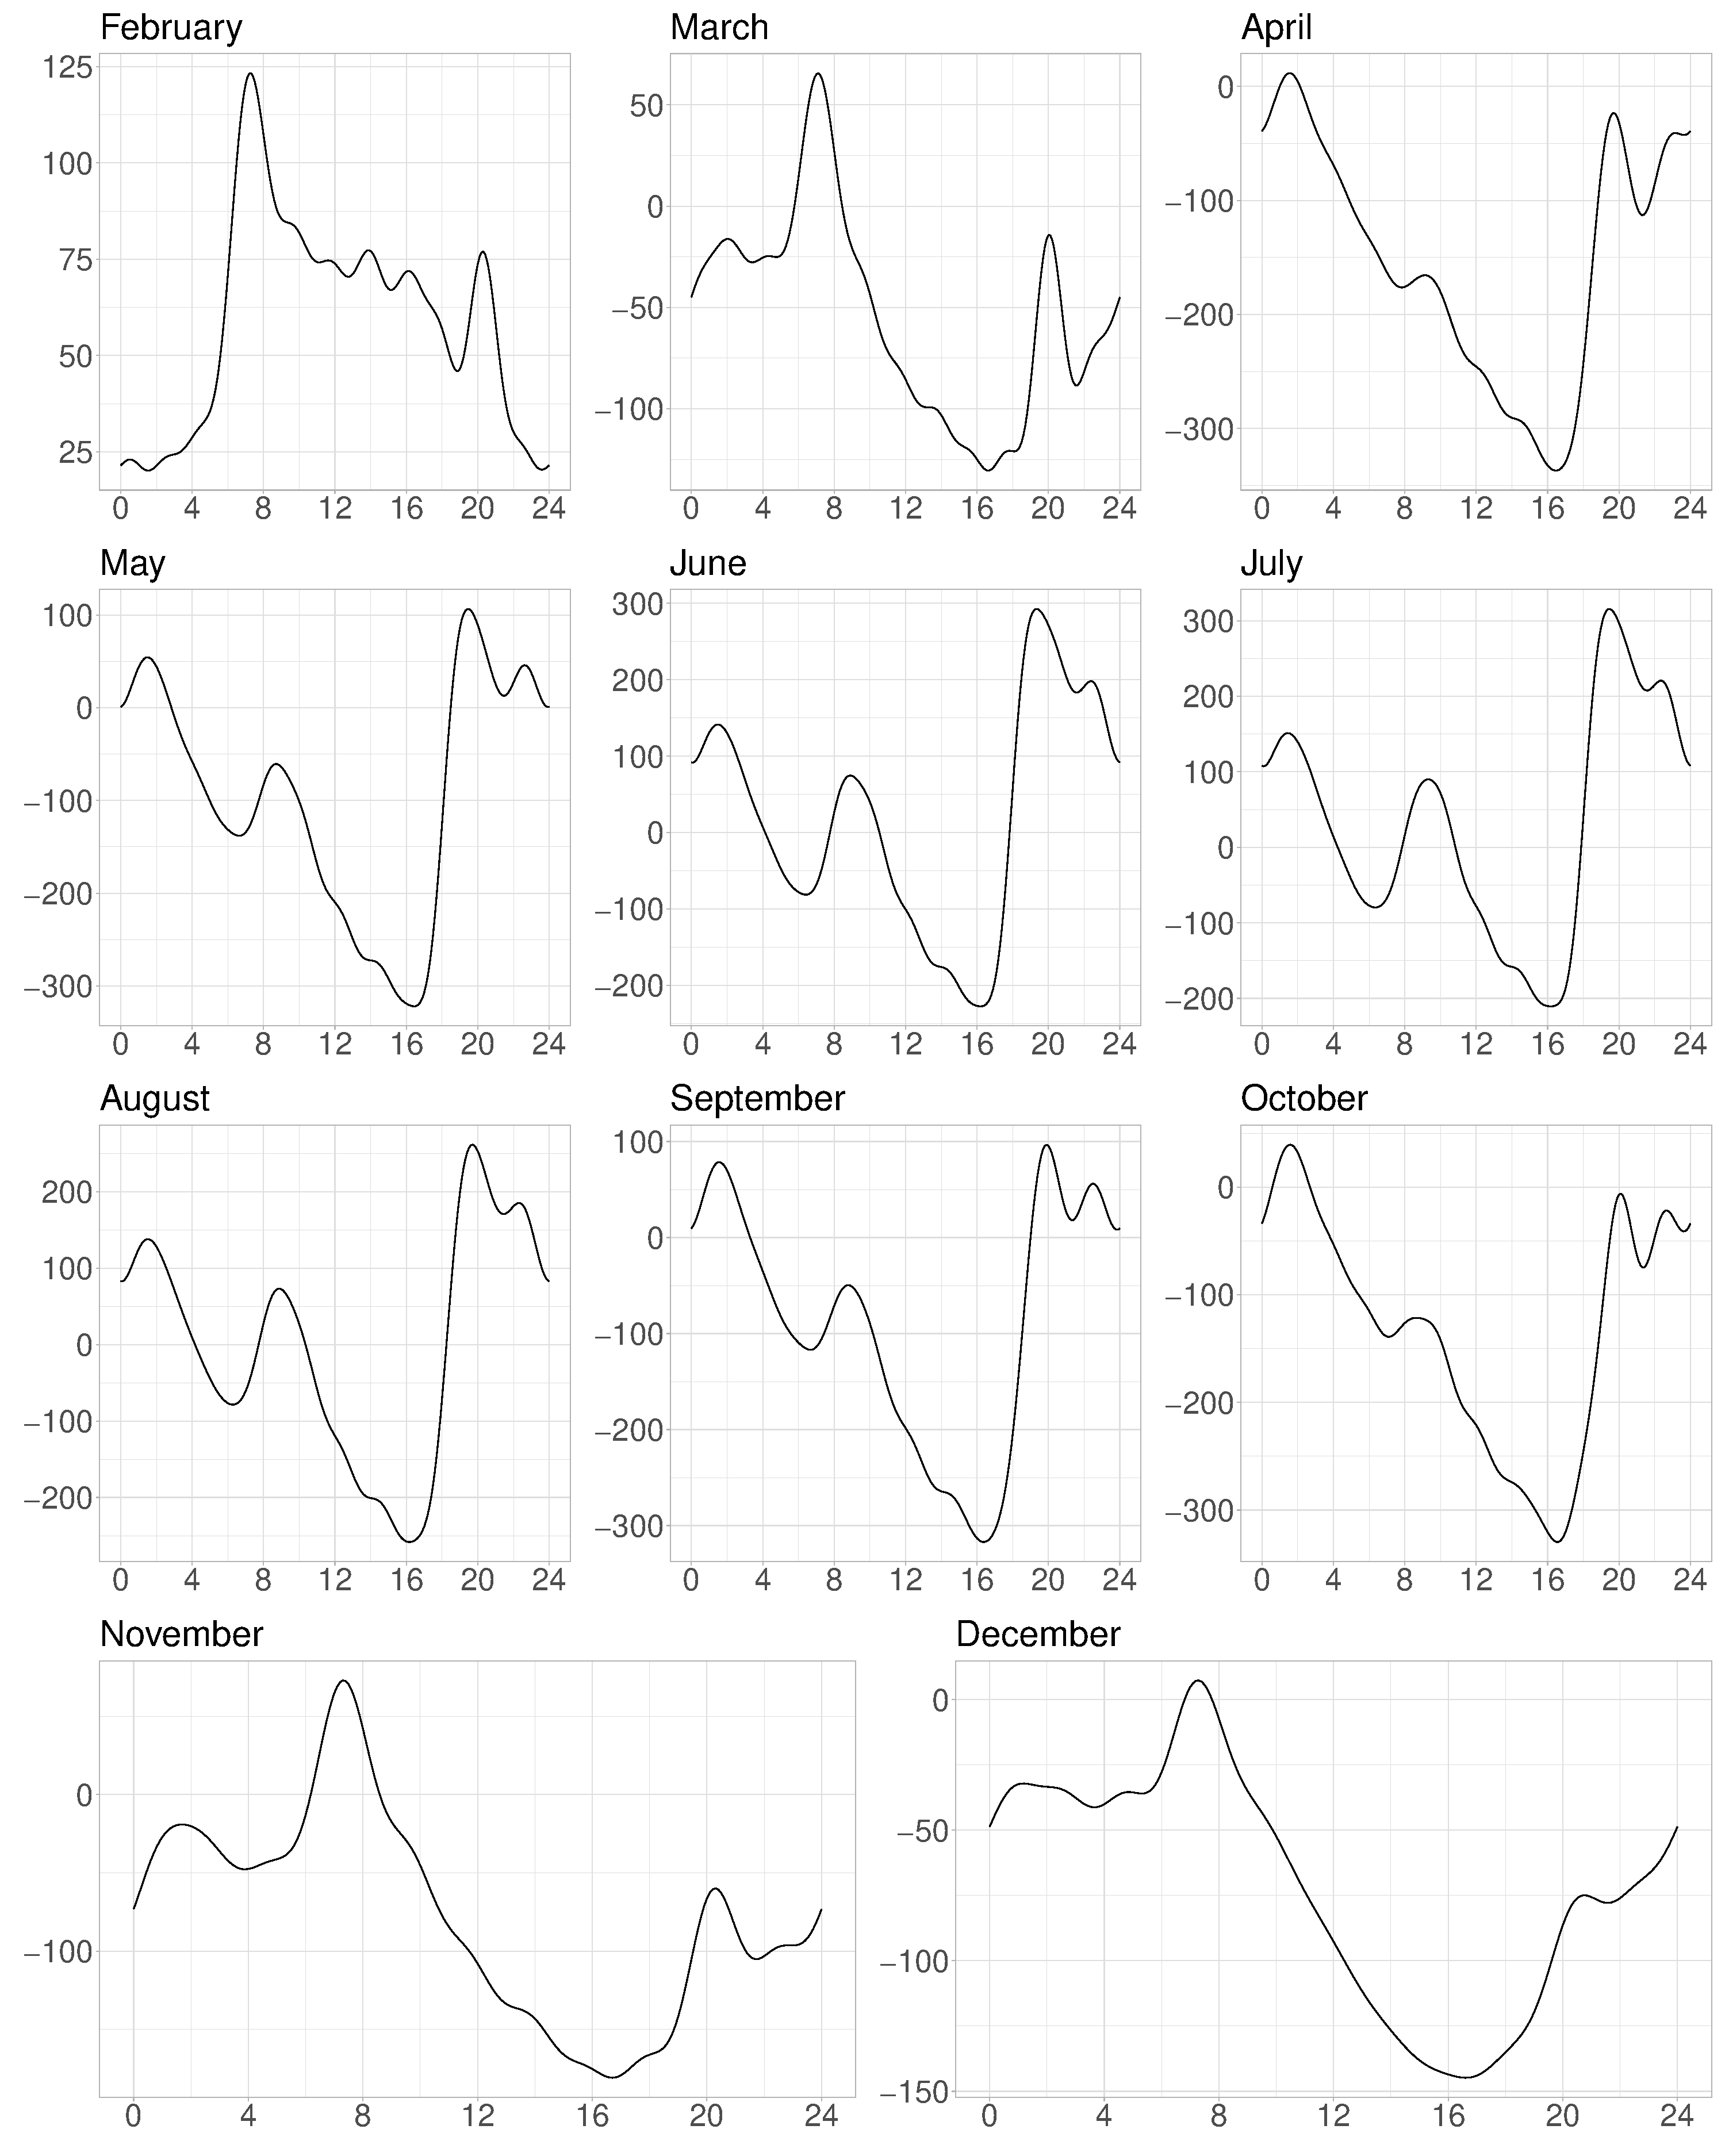
\includegraphics[width=1.1\textwidth]{../Graphics/estimate_months.PDF}
				}
				\caption{Estimates for the months (January as baseline)}
				\label{estimates_months}
			\end{figure}
			
		\subsection{Additional Figures}\label{add_figures}
			\begin{figure}[H]
				\makebox[\textwidth][c]{
					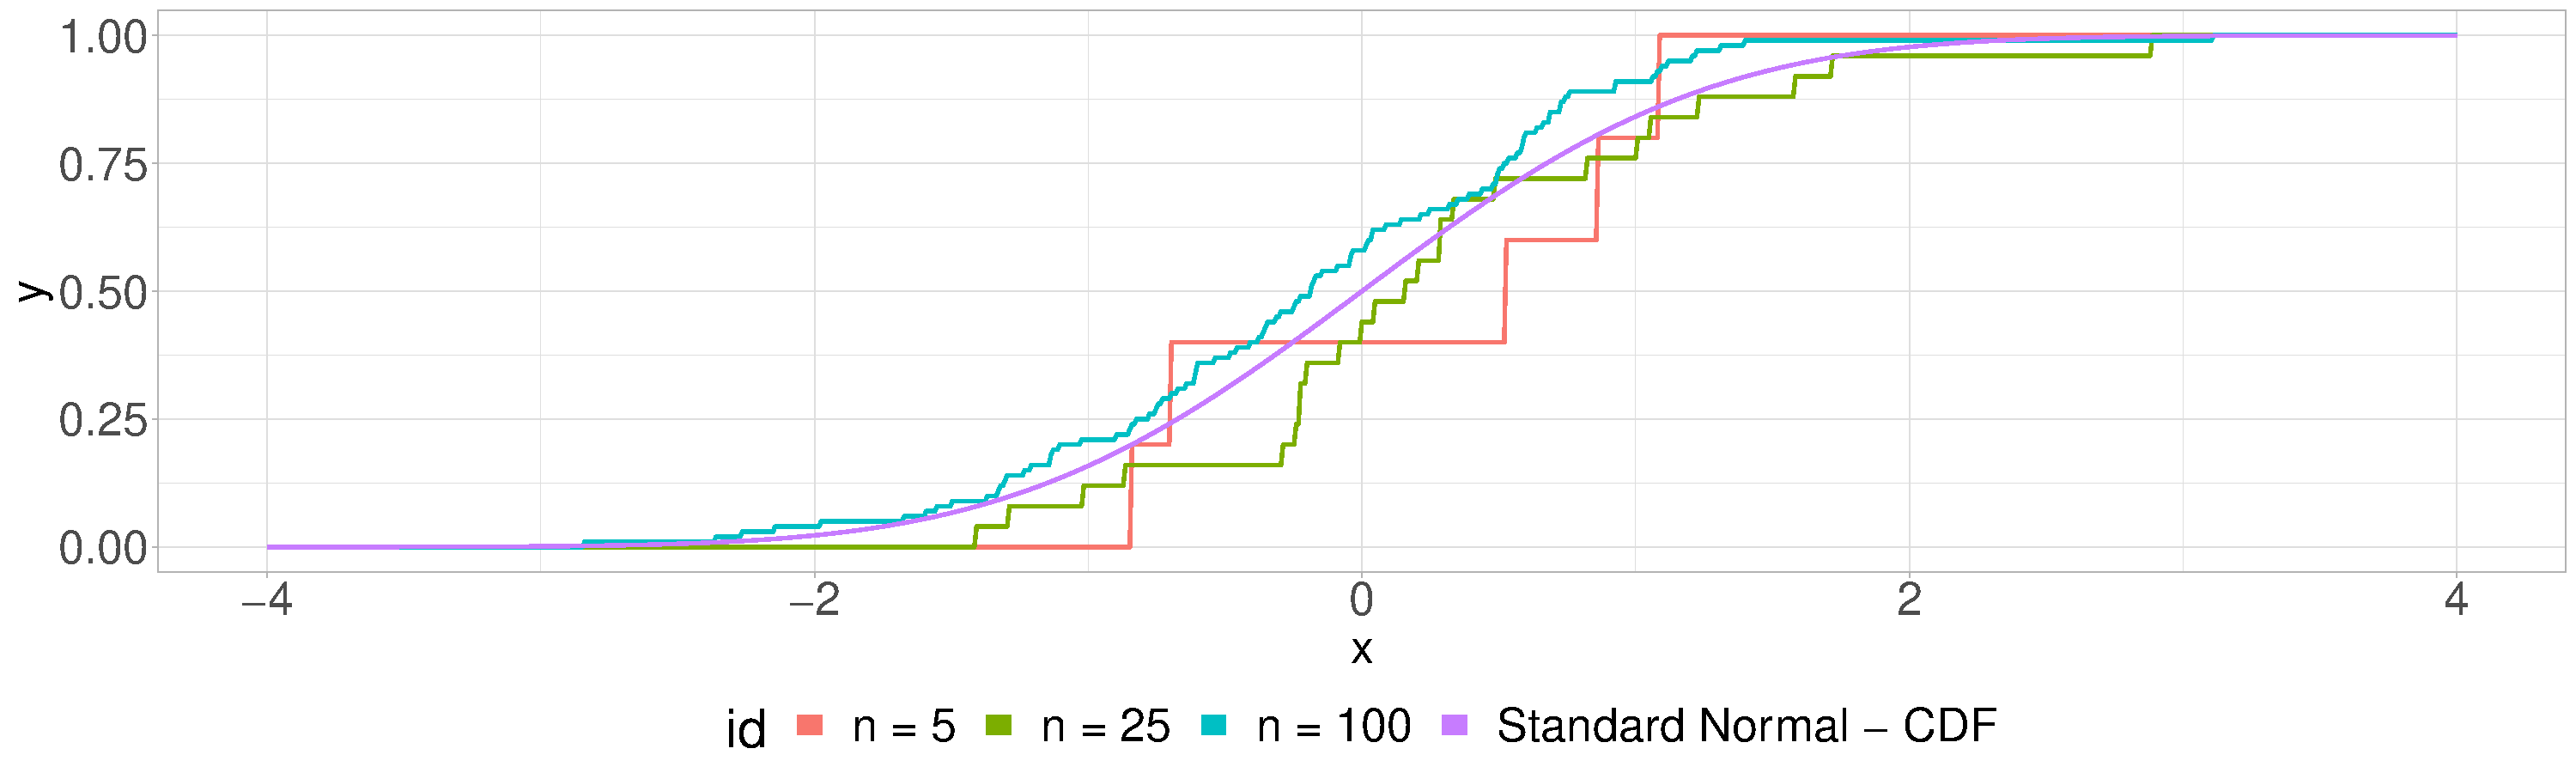
\includegraphics[width = 1.1\textwidth]{../Graphics/ecdf.PDF}
				}
				\caption{Empirical Distribution Functions for different samples drawn from a Standard Normal Distribution}
				\label{ecdf_plot}
			\end{figure}
		
			\begin{figure}[H]
				\makebox[\textwidth][c]{
					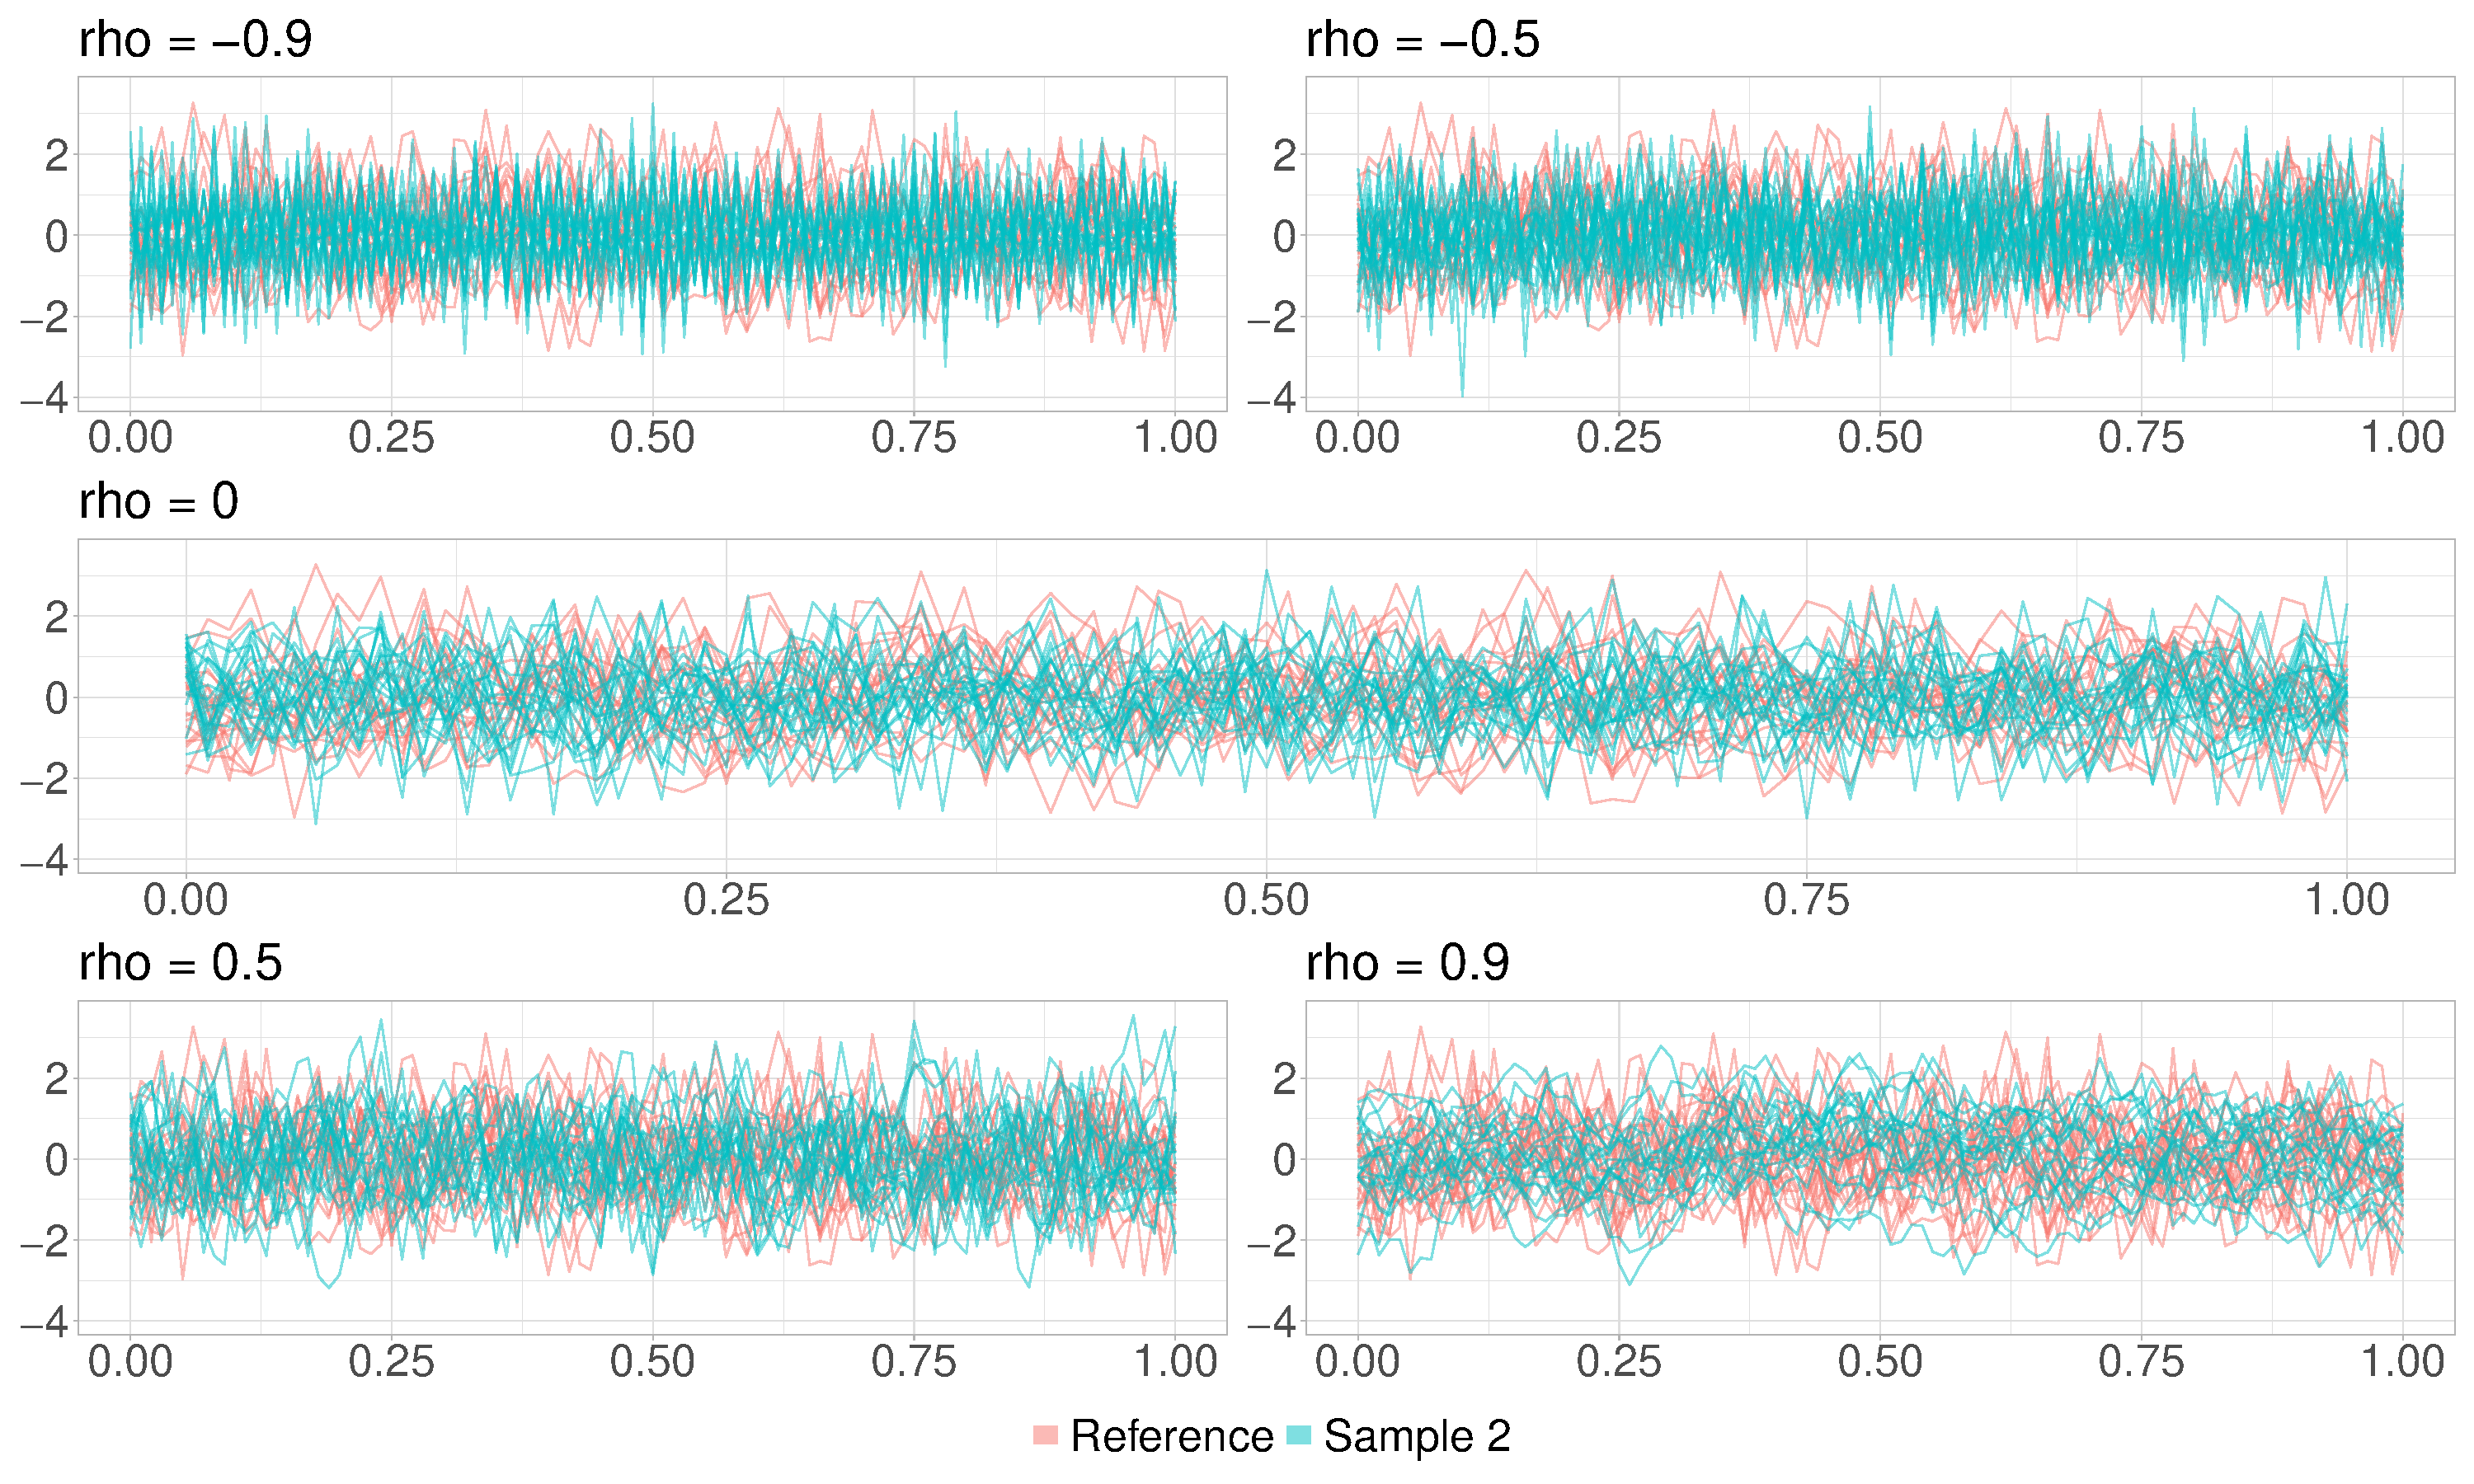
\includegraphics[width=1.1\textwidth]{../Graphics/persistence_comparison.PDF}
				}
				\caption{Original Samples for Persistence Test}
				\label{persistence_samples}
			\end{figure}
			
		
			\begin{figure}[H]
				\makebox[\textwidth][c]{
					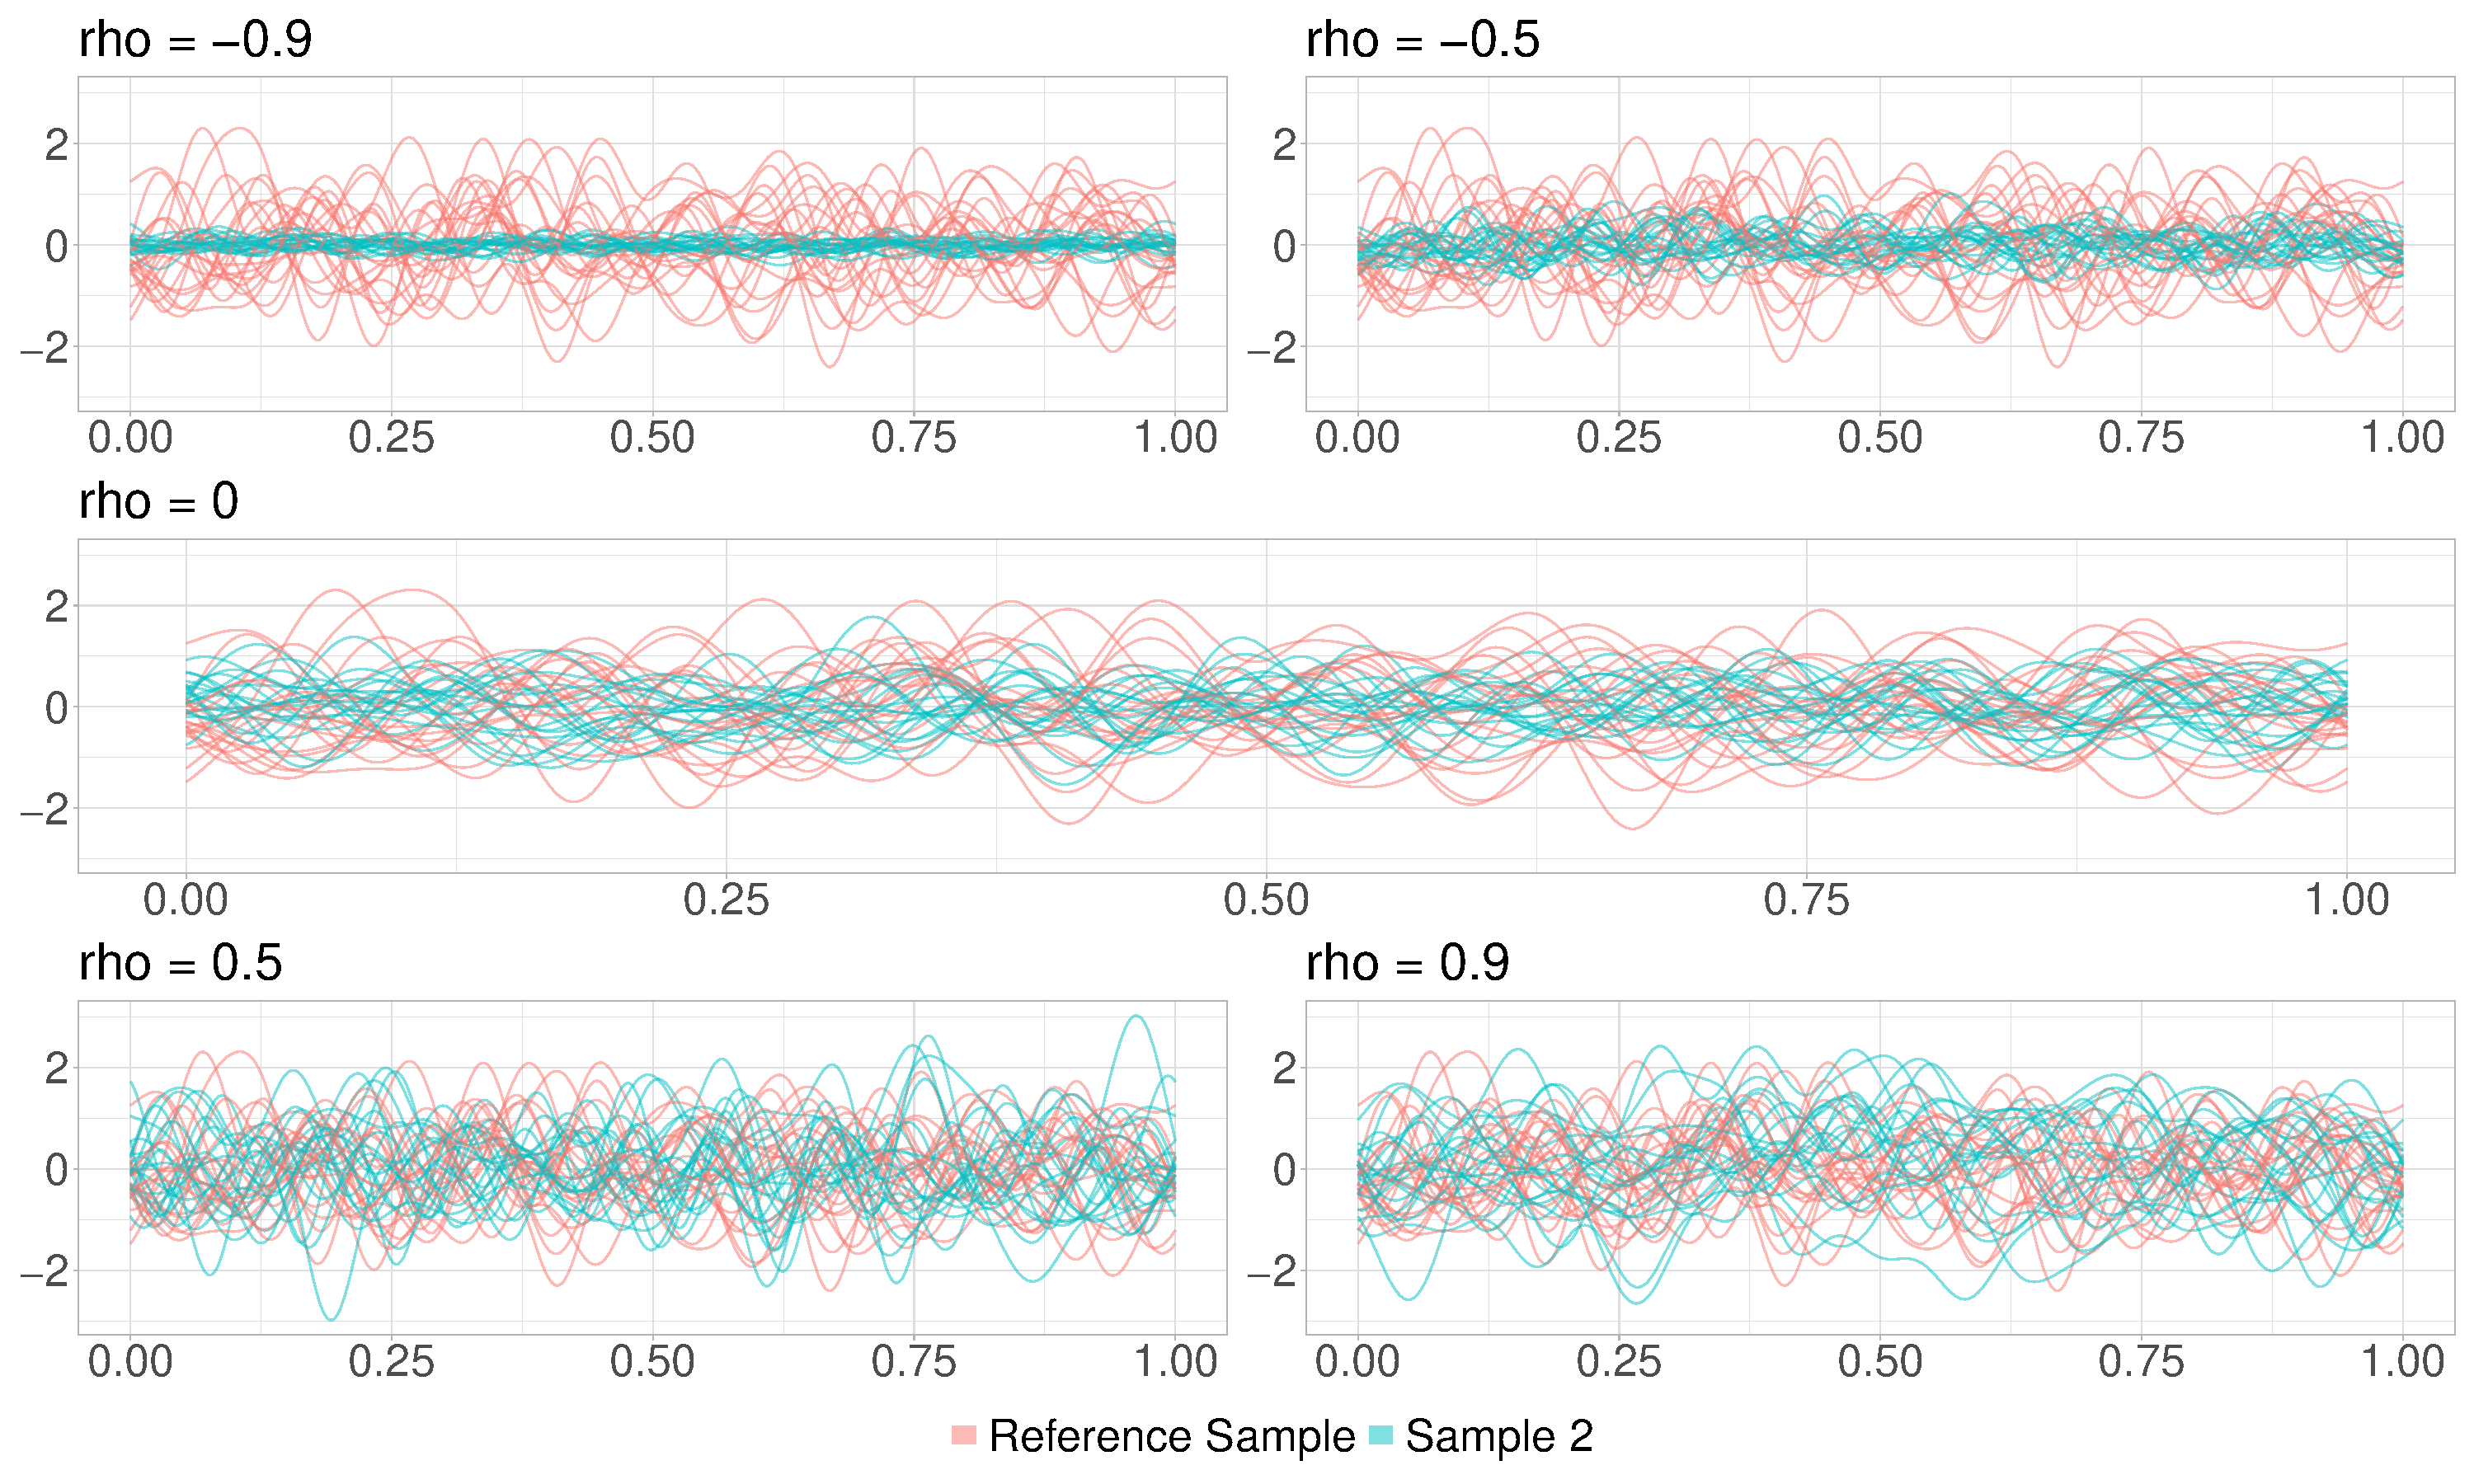
\includegraphics[width=1.1\textwidth]{../Graphics/persistence_comparison_basis.PDF}
				}
				\caption{Samples for Persistence Test fitted using a Fourier Basis with 25 functions}
				\label{persistence_samples_basis_problem}
			\end{figure}
		
		
		
	\newpage
	\thispagestyle{empty}
	\section*{Versicherung an Eides statt}	
	
		\vspace{3cm}
		
		Ich versichere hiermit, dass ich die vorstehende Masterarbeit
		selbstständig verfasst und keine anderen als die angegebenen Quellen
		und Hilfsmittel benutzt habe, dass die vorgelegte Arbeit noch an keiner
		anderen Hochschule zur Prüfung vorgelegt wurde und dass sie weder
		ganz noch in Teilen bereits veröffentlicht wurde. Wörtliche Zitate und
		Stellen, die anderen Werken dem Sinn nach entnommen sind, habe ich
		in jedem einzelnen Fall kenntlich gemacht.
		
		\vspace{2cm}
		Bonn, XX.07.2021 \hrulefill \\
		\hspace*{0mm}Jakob R. Juergens
		
		\vspace{\fill}
\end{document}